\documentclass[]{article}

\usepackage{graphicx,type1cm,eso-pic,color}

\makeatletter
          \AddToShipoutPicture{
            \setlength{\@tempdimb}{.95\paperwidth}
            \setlength{\@tempdimc}{.5\paperheight}
            \setlength{\unitlength}{1pt}
            \put(\strip@pt\@tempdimb,\strip@pt\@tempdimc){
        \makebox(0,0){\rotatebox{-90}{\textcolor[gray]{0.90}
        {\fontsize{.65cm}{.5cm}\selectfont{\rm BCAM - Basque Center for Applied Mathematics}}}}
            }
        }
          \AddToShipoutPicture{
            \setlength{\@tempdimb}{.50\paperwidth}
            \setlength{\@tempdimc}{.95\paperheight}
            \setlength{\unitlength}{1pt}
            \put(\strip@pt\@tempdimb,\strip@pt\@tempdimc){
        \makebox(0,0){\rotatebox{0}{\textcolor[gray]{0.90}
        {\fontsize{.5cm}{.5cm}\selectfont{\rm Azti Course 2016 by Dae-Jin Lee}}}}
            }
        }
\makeatother

\def\tightlist{}

\usepackage{lmodern}
\usepackage{amssymb,amsmath}
\usepackage{ifxetex,ifluatex}
\usepackage{fixltx2e} % provides \textsubscript
\ifnum 0\ifxetex 1\fi\ifluatex 1\fi=0 % if pdftex
  \usepackage[T1]{fontenc}
  \usepackage[utf8]{inputenc}
\else % if luatex or xelatex
  \ifxetex
    \usepackage{mathspec}
    \usepackage{xltxtra,xunicode}
  \else
    \usepackage{fontspec}
  \fi
  \defaultfontfeatures{Mapping=tex-text,Scale=MatchLowercase}
  \newcommand{\euro}{???}
\fi
% use upquote if available, for straight quotes in verbatim environments
\IfFileExists{upquote.sty}{\usepackage{upquote}}{}
% use microtype if available
\IfFileExists{microtype.sty}{%
\usepackage{microtype}
\UseMicrotypeSet[protrusion]{basicmath} % disable protrusion for tt fonts
}{}
\usepackage{color}
\usepackage{fancyvrb}
\newcommand{\VerbBar}{|}
\newcommand{\VERB}{\Verb[commandchars=\\\{\}]}
\DefineVerbatimEnvironment{Highlighting}{Verbatim}{commandchars=\\\{\}}
% Add ',fontsize=\small' for more characters per line
\usepackage{framed}
\definecolor{shadecolor}{RGB}{248,248,248}
\newenvironment{Shaded}{\begin{snugshade}}{\end{snugshade}}
\newcommand{\KeywordTok}[1]{\textcolor[rgb]{0.13,0.29,0.53}{\textbf{{#1}}}}
\newcommand{\DataTypeTok}[1]{\textcolor[rgb]{0.13,0.29,0.53}{{#1}}}
\newcommand{\DecValTok}[1]{\textcolor[rgb]{0.00,0.00,0.81}{{#1}}}
\newcommand{\BaseNTok}[1]{\textcolor[rgb]{0.00,0.00,0.81}{{#1}}}
\newcommand{\FloatTok}[1]{\textcolor[rgb]{0.00,0.00,0.81}{{#1}}}
\newcommand{\ConstantTok}[1]{\textcolor[rgb]{0.00,0.00,0.00}{{#1}}}
\newcommand{\CharTok}[1]{\textcolor[rgb]{0.31,0.60,0.02}{{#1}}}
\newcommand{\SpecialCharTok}[1]{\textcolor[rgb]{0.00,0.00,0.00}{{#1}}}
\newcommand{\StringTok}[1]{\textcolor[rgb]{0.31,0.60,0.02}{{#1}}}
\newcommand{\VerbatimStringTok}[1]{\textcolor[rgb]{0.31,0.60,0.02}{{#1}}}
\newcommand{\SpecialStringTok}[1]{\textcolor[rgb]{0.31,0.60,0.02}{{#1}}}
\newcommand{\ImportTok}[1]{{#1}}
\newcommand{\CommentTok}[1]{\textcolor[rgb]{0.56,0.35,0.01}{\textit{{#1}}}}
\newcommand{\DocumentationTok}[1]{\textcolor[rgb]{0.56,0.35,0.01}{\textbf{\textit{{#1}}}}}
\newcommand{\AnnotationTok}[1]{\textcolor[rgb]{0.56,0.35,0.01}{\textbf{\textit{{#1}}}}}
\newcommand{\CommentVarTok}[1]{\textcolor[rgb]{0.56,0.35,0.01}{\textbf{\textit{{#1}}}}}
\newcommand{\OtherTok}[1]{\textcolor[rgb]{0.56,0.35,0.01}{{#1}}}
\newcommand{\FunctionTok}[1]{\textcolor[rgb]{0.00,0.00,0.00}{{#1}}}
\newcommand{\VariableTok}[1]{\textcolor[rgb]{0.00,0.00,0.00}{{#1}}}
\newcommand{\ControlFlowTok}[1]{\textcolor[rgb]{0.13,0.29,0.53}{\textbf{{#1}}}}
\newcommand{\OperatorTok}[1]{\textcolor[rgb]{0.81,0.36,0.00}{\textbf{{#1}}}}
\newcommand{\BuiltInTok}[1]{{#1}}
\newcommand{\ExtensionTok}[1]{{#1}}
\newcommand{\PreprocessorTok}[1]{\textcolor[rgb]{0.56,0.35,0.01}{\textit{{#1}}}}
\newcommand{\AttributeTok}[1]{\textcolor[rgb]{0.77,0.63,0.00}{{#1}}}
\newcommand{\RegionMarkerTok}[1]{{#1}}
\newcommand{\InformationTok}[1]{\textcolor[rgb]{0.56,0.35,0.01}{\textbf{\textit{{#1}}}}}
\newcommand{\WarningTok}[1]{\textcolor[rgb]{0.56,0.35,0.01}{\textbf{\textit{{#1}}}}}
\newcommand{\AlertTok}[1]{\textcolor[rgb]{0.94,0.16,0.16}{{#1}}}
\newcommand{\ErrorTok}[1]{\textcolor[rgb]{0.64,0.00,0.00}{\textbf{{#1}}}}
\newcommand{\NormalTok}[1]{{#1}}
\usepackage{longtable,booktabs}
\usepackage{graphicx}
\makeatletter
\def\maxwidth{\ifdim\Gin@nat@width>\linewidth\linewidth\else\Gin@nat@width\fi}
\def\maxheight{\ifdim\Gin@nat@height>\textheight\textheight\else\Gin@nat@height\fi}
\makeatother
% Scale images if necessary, so that they will not overflow the page
% margins by default, and it is still possible to overwrite the defaults
% using explicit options in \includegraphics[width, height, ...]{}
\setkeys{Gin}{width=\maxwidth,height=\maxheight,keepaspectratio}
\ifxetex
  \usepackage[setpagesize=false, % page size defined by xetex
              unicode=false, % unicode breaks when used with xetex
              xetex]{hyperref}
\else
  \usepackage[unicode=true]{hyperref}
\fi
\hypersetup{breaklinks=true,
            bookmarks=true,
            pdfauthor={Dae-Jin Lee \textless{} dlee@bcamath.org \textgreater{}},
            pdftitle={Introduction to R statistical software},
            colorlinks=true,
            citecolor=blue,
            urlcolor=blue,
            linkcolor=magenta,
            pdfborder={0 0 0}}
\urlstyle{same}  % don't use monospace font for urls
\setlength{\parindent}{0pt}
\setlength{\parskip}{6pt plus 2pt minus 1pt}
\setlength{\emergencystretch}{3em}  % prevent overfull lines
\setcounter{secnumdepth}{5}

\title{\textbf{Introduction to \texttt{R} statistical software}\\\vspace{0.5em}{\large BCAM - Basque Center for Applied Mathematics, Applied Statistics}}
\author{Dae-Jin Lee \textless{}
\href{mailto:dlee@bcamath.org}{\nolinkurl{dlee@bcamath.org}}
\textgreater{}}
\date{Azti - Tecnalia}

\usepackage{amsfonts}
\usepackage{amsmath}
\usepackage{amssymb}
\usepackage{natbib}
%\usepackage[T1]{fontenc}
\usepackage{latexsym}
\usepackage{graphicx}
\usepackage{caption}
\usepackage{subcaption}
\usepackage{color}
\usepackage{algorithm2e}
%%
%     Definitions
%
\newcommand{\tri}{\bigtriangleup}
\newcommand{\Xp}{X^\prime}
\newcommand{\E}{\mbox{E}}
\newcommand{\Hh}{\mbox{H}}
\newcommand{\V}{\mbox{Var}}
\newcommand{\tr}{\mbox{tr}}
\newcommand{\CV}{\mbox{CV}}
\newcommand{\GCV}{\mbox{GCV}}
\newcommand{\AIC}{\mbox{AIC}}
\newcommand{\ph}{\phantom{0}}
\newcommand{\half}{\mbox{${1\over2}$}}
\newcommand{\bfzero}{\boldsymbol{0}}
\newcommand{\bfone}{\boldsymbol{1}}

\newcommand{\bfa}{\boldsymbol{a}}
\newcommand{\bfb}{\boldsymbol{b}}
\newcommand{\bfe}{\boldsymbol{e}}
\newcommand{\bff}{\boldsymbol{f}}
\newcommand{\bfg}{\boldsymbol{g}}
\newcommand{\bfs}{\boldsymbol{s}}
\newcommand{\bfu}{\boldsymbol{u}}
\newcommand{\bfx}{\boldsymbol{x}}
\newcommand{\bfy}{\boldsymbol{y}}
\newcommand{\bfz}{\boldsymbol{z}}

\newcommand{\bfA}{\boldsymbol{A}}
\newcommand{\bfB}{\boldsymbol{B}}
\newcommand{\bfC}{\boldsymbol{C}}
\newcommand{\bfD}{\boldsymbol{D}}
\newcommand{\bfF}{\boldsymbol{F}}
\newcommand{\bfG}{\boldsymbol{G}}
\newcommand{\bfH}{\boldsymbol{H}}
\newcommand{\bfI}{\boldsymbol{I}}
\newcommand{\bfM}{\boldsymbol{M}}
\newcommand{\bfP}{\boldsymbol{P}}
\newcommand{\bfQ}{\boldsymbol{Q}}
\newcommand{\bfR}{\boldsymbol{R}}
\newcommand{\bfS}{\boldsymbol{S}}
\newcommand{\bfT}{\boldsymbol{T}}
\newcommand{\bfU}{\boldsymbol{U}}
\newcommand{\bfV}{\boldsymbol{V}}
\newcommand{\bfW}{\boldsymbol{W}}
\newcommand{\bfX}{\boldsymbol{X}}
\newcommand{\bfY}{\boldsymbol{Y}}
\newcommand{\bfZ}{\boldsymbol{Z}}


\newcommand{\bfalpha}{\boldsymbol{\alpha}}
\newcommand{\bfbeta}{\boldsymbol{\beta}}
\newcommand{\bfepsilon}{\boldsymbol{\epsilon}}
\newcommand{\bfgamma}{\boldsymbol{\gamma}}
\newcommand{\bfGamma}{\boldsymbol{\Gamma}}
\newcommand{\bfmu}{\boldsymbol{\mu}}
\newcommand{\bfeta}{\boldsymbol{\eta}}
\newcommand{\bfrho}{\boldsymbol{\rho}}
\newcommand{\bftheta}{\boldsymbol{\theta}}
\newcommand{\bfxi}{\boldsymbol{\xi}}
\newcommand{\bftau}{\boldsymbol{\tau}}
\newcommand{\bflambda}{\boldsymbol{\lambda}}
\newcommand{\bfsigma}{\boldsymbol{\sigma}}
\newcommand{\bfLambda}{\boldsymbol{\Lambda}}
\newcommand{\bfSigma}{\boldsymbol{\Sigma}}

\renewcommand{\theequation}{\thesection.\arabic{equation}}
\numberwithin{equation}{section}

\begin{document}
\maketitle

{
\hypersetup{linkcolor=black}
\setcounter{tocdepth}{2}
\tableofcontents
}
\begin{center}\rule{0.5\linewidth}{\linethickness}\end{center}

This course is an introduction to statistical software \texttt{R}. The
course will introduce the student to the basics of using \texttt{R} for
statistical programming, computation, graphics, and basic statistical
modeling.

\textbf{Objectives:}

\begin{itemize}
\tightlist
\item
  Use \texttt{R} for basic data analysis.
\item
  Write functions in and use \texttt{R} in efficient way,
\item
  Perform basic statistical analysis and basic statistical models.
\end{itemize}

\textbf{Pre-requisites:}

There are no formal prerequisites, but some basic knowledge of
statistics is expected. The intended audience is anyone who needs a
flexible statistical environment for their research. Any prior knowledge
of \texttt{R} is not expected.

\textbf{Compulsory:}

\begin{itemize}
\tightlist
\item
  Bring your laptop with the latest version of \texttt{R} installed.
  Download it \href{https://cran.r-project.org/}{here}
\item
  Rstudio is a user-friendly interface. Download it
  \href{https://www.rstudio.com/products/rstudio/download/}{here}
  \textbf{Highly recommended!!!}
\item
  Internet connection to download the material and install some
  packages.
\end{itemize}

\begin{center}\rule{0.5\linewidth}{\linethickness}\end{center}

\section{\texorpdfstring{Introduction to the \texttt{R}
language}{Introduction to the R language}}\label{introduction-to-the-r-language}

\begin{itemize}
\item
  \texttt{R} is a free software environment for statistical computing
  and graphics \url{http://www.r-project.org}
\item
  \texttt{R} is a command-driven statistical package.
\item
  The most important reasons to use \texttt{R} are:

  \begin{itemize}
  \item
    \texttt{R} is free and multiplatform (Windows/Linux/MACos)
  \item
    \texttt{R} allows you to do all the statistical
    tests/models/analysis you need :)
  \item
    Excellent graphics and programming capabilities
  \item
    Growing community of users and developers
  \item
    Lots of online resources
  \end{itemize}
\item
  Statistical features:

  \begin{itemize}
  \item
    Graphical Techniques (Exploratory Data Analysis)
  \item
    Linear and non-linear modeling (linear regression, non-parametric
    regression, smoothing, etc \ldots{})
  \item
    Classical statistical tests
  \item
    Time-series analysis
  \item
    Econometrics
  \item
    Survival analysis
  \item
    Classification and clustering (data mining, machine learning)
  \item
    Optimization and Mathematical Programming
  \item
    Bayesian inference etc \ldots{}.
  \end{itemize}
\end{itemize}

\textbf{Visit} \url{http://cran.r-project.org/web/views} or
\url{http://stackoverflow.com/questions/tagged/r}

\subsection{\texorpdfstring{Start with
\texttt{R}}{Start with R}}\label{start-with-r}

\begin{itemize}
\tightlist
\item
  Get current working directory
\end{itemize}

\begin{Shaded}
\begin{Highlighting}[]
\KeywordTok{getwd}\NormalTok{() }
\end{Highlighting}
\end{Shaded}

\begin{itemize}
\tightlist
\item
  list the objects in the current workspace
\end{itemize}

\begin{Shaded}
\begin{Highlighting}[]
\KeywordTok{ls}\NormalTok{()}
\end{Highlighting}
\end{Shaded}

\begin{itemize}
\tightlist
\item
  Set working directory
\end{itemize}

\begin{Shaded}
\begin{Highlighting}[]
\KeywordTok{setwd}\NormalTok{(}\StringTok{"/Users/dlee"}\NormalTok{) }
\end{Highlighting}
\end{Shaded}

\begin{itemize}
\tightlist
\item
  work with your previous commands
\end{itemize}

\begin{Shaded}
\begin{Highlighting}[]
\KeywordTok{history}\NormalTok{() }\CommentTok{# display last 25 commands}
\KeywordTok{history}\NormalTok{(}\DataTypeTok{max.show=}\OtherTok{Inf}\NormalTok{) }\CommentTok{# display all previous commands}
\end{Highlighting}
\end{Shaded}

\begin{itemize}
\tightlist
\item
  save your command history
\end{itemize}

\begin{Shaded}
\begin{Highlighting}[]
\KeywordTok{savehistory}\NormalTok{(}\DataTypeTok{file=}\StringTok{"myfile"}\NormalTok{) }\CommentTok{# default is ".Rhistory"}
\end{Highlighting}
\end{Shaded}

\begin{itemize}
\tightlist
\item
  recall your command history
\end{itemize}

\begin{Shaded}
\begin{Highlighting}[]
\KeywordTok{loadhistory}\NormalTok{(}\DataTypeTok{file=}\StringTok{"myfile"}\NormalTok{) }\CommentTok{# default is ".Rhistory"}
\end{Highlighting}
\end{Shaded}

\begin{itemize}
\tightlist
\item
  save the workspace to the file \texttt{.RData}
\end{itemize}

\begin{Shaded}
\begin{Highlighting}[]
\KeywordTok{save.image}\NormalTok{()}
\end{Highlighting}
\end{Shaded}

\begin{itemize}
\tightlist
\item
  save specific objects to a file if you don't specify the path, the cwd
  is assumed
\end{itemize}

\begin{Shaded}
\begin{Highlighting}[]
\KeywordTok{save}\NormalTok{(<object list>,}\DataTypeTok{file=}\StringTok{"myfile.RData"}\NormalTok{) }
\end{Highlighting}
\end{Shaded}

\begin{itemize}
\tightlist
\item
  load a workspace into the current session
\end{itemize}

\begin{Shaded}
\begin{Highlighting}[]
\KeywordTok{load}\NormalTok{(}\StringTok{"myfile.RData"}\NormalTok{) }
\end{Highlighting}
\end{Shaded}

\begin{itemize}
\tightlist
\item
  quit \texttt{R}. You will be prompted to save the workspace.
\end{itemize}

\begin{Shaded}
\begin{Highlighting}[]
\KeywordTok{q}\NormalTok{()}
\end{Highlighting}
\end{Shaded}

\subsection{\texorpdfstring{Install and load an \texttt{R}
library}{Install and load an R library}}\label{install-and-load-an-r-library}

\begin{Shaded}
\begin{Highlighting}[]
\KeywordTok{install.packages}\NormalTok{(}\StringTok{"DAAG"}\NormalTok{) }\CommentTok{# (Data Analysis And Graphics)}
\end{Highlighting}
\end{Shaded}

\begin{itemize}
\tightlist
\item
  Once installed the package, load it
\end{itemize}

\begin{Shaded}
\begin{Highlighting}[]
\KeywordTok{library}\NormalTok{(DAAG) }\CommentTok{# or require(DAAG)}
\end{Highlighting}
\end{Shaded}

\begin{center}\rule{0.5\linewidth}{\linethickness}\end{center}

\subsection{Reading data}\label{reading-data}

The \texttt{R} console

\begin{Shaded}
\begin{Highlighting}[]
\NormalTok{x <-}\StringTok{ }\KeywordTok{c}\NormalTok{(}\FloatTok{7.82}\NormalTok{,}\FloatTok{8.00}\NormalTok{,}\FloatTok{7.95}\NormalTok{) }\CommentTok{# c means "combine"}
\NormalTok{x}
\end{Highlighting}
\end{Shaded}

\begin{verbatim}
## [1] 7.82 8.00 7.95
\end{verbatim}

A quicker way is to use \texttt{scan()}

\begin{Shaded}
\begin{Highlighting}[]
\NormalTok{x <-}\StringTok{ }\KeywordTok{scan}\NormalTok{()  }\CommentTok{# enter a number followed by return and blank line to end}
\DecValTok{1}\NormalTok{:}\StringTok{ }\FloatTok{7.82}
\DecValTok{2}\NormalTok{:}\StringTok{ }\FloatTok{8.00}
\DecValTok{3}\NormalTok{:}\StringTok{ }\FloatTok{7.95}
\DecValTok{4}\NormalTok{:}\StringTok{ }
\NormalTok{Read }\DecValTok{3} \NormalTok{items}
\end{Highlighting}
\end{Shaded}

To create a character vector use \texttt{""}

\begin{Shaded}
\begin{Highlighting}[]
\NormalTok{id <-}\StringTok{ }\KeywordTok{c}\NormalTok{(}\StringTok{"John"}\NormalTok{,}\StringTok{"Paul"}\NormalTok{,}\StringTok{"George"}\NormalTok{,}\StringTok{"Ringo"}\NormalTok{)}
\end{Highlighting}
\end{Shaded}

To read a character vector

\begin{Shaded}
\begin{Highlighting}[]
\NormalTok{id <-}\StringTok{ }\KeywordTok{scan}\NormalTok{(,}\StringTok{""}\NormalTok{)}
\DecValTok{1}\NormalTok{:}\StringTok{ }\NormalTok{John}
\DecValTok{2}\NormalTok{:}\StringTok{ }\NormalTok{Paul}
\DecValTok{3}\NormalTok{:}\StringTok{ }\NormalTok{George}
\DecValTok{4}\NormalTok{:}\StringTok{ }\NormalTok{Ringo}
\DecValTok{5}\NormalTok{:}\StringTok{ }
\NormalTok{Read }\DecValTok{4} \NormalTok{items  }
\end{Highlighting}
\end{Shaded}

\begin{Shaded}
\begin{Highlighting}[]
\NormalTok{id}
\end{Highlighting}
\end{Shaded}

\begin{verbatim}
## [1] "John"   "Paul"   "George" "Ringo"
\end{verbatim}

\subsection{Data Import}\label{data-import}

In most situations, we need to read data from a separate data file.
There are several methods for doing this.

\begin{itemize}
\tightlist
\item
  \texttt{scan()} (see \texttt{?scan} for help)
\end{itemize}

\begin{Shaded}
\begin{Highlighting}[]
\KeywordTok{cat}\NormalTok{(}\StringTok{"Example:"}\NormalTok{, }\StringTok{"2 3 5 7"}\NormalTok{, }\StringTok{"11 13 17"}\NormalTok{, }\DataTypeTok{file =} \StringTok{"ex.txt"}\NormalTok{, }\DataTypeTok{sep =} \StringTok{"}\CharTok{\textbackslash{}n}\StringTok{"}\NormalTok{) }\CommentTok{# creates ex.txt}
\KeywordTok{scan}\NormalTok{(}\StringTok{"ex.txt"}\NormalTok{, }\DataTypeTok{skip =} \DecValTok{1}\NormalTok{)}
\end{Highlighting}
\end{Shaded}

\begin{verbatim}
## [1]  2  3  5  7 11 13 17
\end{verbatim}

\begin{Shaded}
\begin{Highlighting}[]
\KeywordTok{scan}\NormalTok{(}\StringTok{"ex.txt"}\NormalTok{, }\DataTypeTok{skip =} \DecValTok{1}\NormalTok{, }\DataTypeTok{nlines =} \DecValTok{1}\NormalTok{) }\CommentTok{# only 1 line after the skipped one}
\end{Highlighting}
\end{Shaded}

\begin{verbatim}
## [1] 2 3 5 7
\end{verbatim}

\begin{Shaded}
\begin{Highlighting}[]
\KeywordTok{unlink}\NormalTok{(}\StringTok{"ex.data"}\NormalTok{) }\CommentTok{# tidy up}
\end{Highlighting}
\end{Shaded}

\begin{itemize}
\item
  Several formats are available (\texttt{.txt}, \texttt{.csv},
  \texttt{.xls}, \texttt{.xlsx}, \texttt{SAS}, \texttt{Stata},
  etc\ldots{})
\item
  Some \texttt{R} libraries to import data are
\end{itemize}

\begin{Shaded}
\begin{Highlighting}[]
\KeywordTok{library}\NormalTok{(gdata)}
\KeywordTok{library}\NormalTok{(foreign)}
\end{Highlighting}
\end{Shaded}

\bigskip

\begin{itemize}
\tightlist
\item
  Read data from a \texttt{.txt} or \texttt{.csv} files
\end{itemize}

\begin{Shaded}
\begin{Highlighting}[]
\NormalTok{mydata1 =}\StringTok{ }\KeywordTok{read.table}\NormalTok{(}\StringTok{"mydata.txt"}\NormalTok{) }
\NormalTok{mydata2 =}\StringTok{ }\KeywordTok{read.csv}\NormalTok{(}\StringTok{"mydata.csv"}\NormalTok{)  }
\end{Highlighting}
\end{Shaded}

\begin{itemize}
\tightlist
\item
  Other formats \texttt{.xls} and \texttt{.xlsx}
\end{itemize}

\begin{Shaded}
\begin{Highlighting}[]
\CommentTok{# read in the worksheet named mysheet}
\NormalTok{mydata <-}\StringTok{ }\KeywordTok{read.xlsx}\NormalTok{(}\StringTok{"myexcel.xlsx"}\NormalTok{, }\DataTypeTok{sheetName =} \StringTok{"mysheet"}\NormalTok{)}
\end{Highlighting}
\end{Shaded}

\begin{center}\rule{0.5\linewidth}{\linethickness}\end{center}

\begin{itemize}
\tightlist
\item
  Minitab, SPSS, SAS or Stata
\end{itemize}

\begin{Shaded}
\begin{Highlighting}[]
\KeywordTok{library}\NormalTok{(foreign)                   }
\NormalTok{mydata =}\StringTok{ }\KeywordTok{read.mtp}\NormalTok{(}\StringTok{"mydata.mtp"}\NormalTok{)  }\CommentTok{# Minitab}
\NormalTok{mydata =}\StringTok{ }\KeywordTok{read.spss}\NormalTok{(}\StringTok{"myfile"}\NormalTok{, }\DataTypeTok{to.data.frame=}\OtherTok{TRUE}\NormalTok{) }\CommentTok{# SPSS}
\NormalTok{mydata =}\StringTok{ }\KeywordTok{read.dta}\NormalTok{(}\StringTok{"mydata.dta"}\NormalTok{) }\CommentTok{# Stata}
\end{Highlighting}
\end{Shaded}

\begin{itemize}
\tightlist
\item
  Or
\end{itemize}

\begin{Shaded}
\begin{Highlighting}[]
\KeywordTok{library}\NormalTok{(Hmisc)}
\NormalTok{mydata =}\StringTok{ }\KeywordTok{spss.get}\NormalTok{(}\StringTok{"mydata.por"}\NormalTok{, }\DataTypeTok{use.value.labels=}\OtherTok{TRUE}\NormalTok{)  }\CommentTok{# SPSS}
\end{Highlighting}
\end{Shaded}

\begin{center}\rule{0.5\linewidth}{\linethickness}\end{center}

\subsection{Exporting data}\label{exporting-data}

\begin{itemize}
\item
  There are numerous methods for exporting \texttt{R} objects into other
  formats . For SPSS, SAS and Stata. you will need to load the
  \texttt{foreign} packages. For Excel, you will need the \texttt{xlsx}
  package.
\item
  Tab delimited text file
\end{itemize}

\begin{Shaded}
\begin{Highlighting}[]
\NormalTok{mtcars}
\NormalTok{?mtcars    }
\KeywordTok{write.table}\NormalTok{(mtcars, }\StringTok{"mydata.txt"}\NormalTok{, }\DataTypeTok{sep=}\StringTok{"}\CharTok{\textbackslash{}t}\StringTok{"}\NormalTok{) }
\end{Highlighting}
\end{Shaded}

\begin{itemize}
\tightlist
\item
  Excel spreadsheet
\end{itemize}

\begin{Shaded}
\begin{Highlighting}[]
\KeywordTok{library}\NormalTok{(xlsx)}
\KeywordTok{write.xlsx}\NormalTok{(mydata, }\StringTok{"mydata.xlsx"}\NormalTok{)}
\end{Highlighting}
\end{Shaded}

\begin{center}\rule{0.5\linewidth}{\linethickness}\end{center}

\subsection{Data vectors}\label{data-vectors}

\begin{itemize}
\item
  Download \texttt{R\ code}
  \href{http://idaejin.github.io/bcam-courses/rbasics/rbasics.R}{here}
\item
  Create a vector of weights and heights
\end{itemize}

\begin{Shaded}
\begin{Highlighting}[]
\NormalTok{weight<-}\KeywordTok{c}\NormalTok{(}\DecValTok{60}\NormalTok{,}\DecValTok{72}\NormalTok{,}\DecValTok{57}\NormalTok{,}\DecValTok{90}\NormalTok{,}\DecValTok{95}\NormalTok{,}\DecValTok{72}\NormalTok{)  }
\KeywordTok{class}\NormalTok{(weight)}
\end{Highlighting}
\end{Shaded}

\begin{verbatim}
## [1] "numeric"
\end{verbatim}

\begin{Shaded}
\begin{Highlighting}[]
\NormalTok{height<-}\KeywordTok{c}\NormalTok{(}\FloatTok{1.75}\NormalTok{,}\FloatTok{1.80}\NormalTok{,}\FloatTok{1.65}\NormalTok{,}\FloatTok{1.90}\NormalTok{,}\FloatTok{1.74}\NormalTok{,}\FloatTok{1.91}\NormalTok{)}
\end{Highlighting}
\end{Shaded}

\begin{itemize}
\tightlist
\item
  calculate Body Mass Index
\end{itemize}

\begin{Shaded}
\begin{Highlighting}[]
\NormalTok{bmi<-}\StringTok{ }\NormalTok{weight/height^}\DecValTok{2}
\NormalTok{bmi}
\end{Highlighting}
\end{Shaded}

\begin{verbatim}
## [1] 19.59184 22.22222 20.93664 24.93075 31.37799 19.73630
\end{verbatim}

\begin{center}\rule{0.5\linewidth}{\linethickness}\end{center}

\subsection{Basic statistics}\label{basic-statistics}

\begin{itemize}
\tightlist
\item
  mean, median, st dev, variance
\end{itemize}

\begin{Shaded}
\begin{Highlighting}[]
\KeywordTok{mean}\NormalTok{(weight) }
\KeywordTok{median}\NormalTok{(weight)}
\KeywordTok{sd}\NormalTok{(weight)}
\KeywordTok{var}\NormalTok{(weight)}
\end{Highlighting}
\end{Shaded}

\begin{itemize}
\tightlist
\item
  summarize data
\end{itemize}

\begin{Shaded}
\begin{Highlighting}[]
\KeywordTok{summary}\NormalTok{(weight)}
\end{Highlighting}
\end{Shaded}

\begin{verbatim}
##    Min. 1st Qu.  Median    Mean 3rd Qu.    Max. 
##   57.00   63.00   72.00   74.33   85.50   95.00
\end{verbatim}

\begin{itemize}
\tightlist
\item
  or
\end{itemize}

\begin{Shaded}
\begin{Highlighting}[]
\KeywordTok{min}\NormalTok{(weight)}
\KeywordTok{max}\NormalTok{(weight)}
\KeywordTok{range}\NormalTok{(weight)}
\KeywordTok{sum}\NormalTok{(weight)}
\KeywordTok{length}\NormalTok{(weight)}
\end{Highlighting}
\end{Shaded}

\begin{itemize}
\tightlist
\item
  Quantiles and percentile
\end{itemize}

There are several quartiles of an observation variable. The first
quartile, or lower quartile, is the value that cuts off the first 25\%
of the data when it is sorted in ascending order. The second quartile,
or median, is the value that cuts off the first 50\%. The third
quartile, or upper quartile, is the value that cuts off the first 75\%.

\begin{Shaded}
\begin{Highlighting}[]
\KeywordTok{quantile}\NormalTok{(weight)}
\end{Highlighting}
\end{Shaded}

\begin{verbatim}
##   0%  25%  50%  75% 100% 
## 57.0 63.0 72.0 85.5 95.0
\end{verbatim}

The \(n^{\rm th}\) percentile of an observation variable is the value
that cuts off the first \(n\) percent of the data values when it is
sorted in ascending order.

\begin{Shaded}
\begin{Highlighting}[]
\KeywordTok{quantile}\NormalTok{(weight,}\KeywordTok{c}\NormalTok{(}\FloatTok{0.32}\NormalTok{,}\FloatTok{0.57}\NormalTok{,}\FloatTok{0.98}\NormalTok{))}
\end{Highlighting}
\end{Shaded}

\begin{verbatim}
##  32%  57%  98% 
## 67.2 72.0 94.5
\end{verbatim}

\begin{itemize}
\tightlist
\item
  Covariance and correlation
\end{itemize}

The \emph{covariance} of two variables \(x\) and \(y\) in a data sample
measures how the two are linearly related. A positive covariance would
indicates a positive linear relationship between the variables, and a
negative covariance would indicate the opposite.

\[
\rm{Cov}(x,y) = \frac{1}{n}\sum_{i=1}^{n}(x_i - \bar{x})(y_i - \bar{y})
\]

\begin{Shaded}
\begin{Highlighting}[]
\KeywordTok{cov}\NormalTok{(weight,height)}
\end{Highlighting}
\end{Shaded}

\begin{verbatim}
## [1] 0.6773333
\end{verbatim}

The \emph{correlation coefficient} of two variables in a data sample is
their covariance divided by the product of their individual standard
deviations. It is a normalized measurement of how the two are linearly
related.

Formally, the sample correlation coefficient is defined by the following
formula, where \(\sigma_x\) and \(\sigma_y\) are the sample standard
deviations, and \(\sigma_xy\) is the covariance.

\[
      \rho_{xy}  = \frac{\sigma_{xy}}{\sigma_x~\sigma_y}
\]

\begin{Shaded}
\begin{Highlighting}[]
\KeywordTok{cor}\NormalTok{(weight,height)}
\end{Highlighting}
\end{Shaded}

\begin{verbatim}
## [1] 0.437934
\end{verbatim}

\begin{center}\rule{0.5\linewidth}{\linethickness}\end{center}

\subsection{Character vectors and factor
variables}\label{character-vectors-and-factor-variables}

\begin{Shaded}
\begin{Highlighting}[]
\NormalTok{subject <-}\StringTok{ }\KeywordTok{c}\NormalTok{(}\StringTok{"John"}\NormalTok{,}\StringTok{"Peter"}\NormalTok{,}\StringTok{"Chris"}\NormalTok{,}\StringTok{"Tony"}\NormalTok{,}\StringTok{"Mary"}\NormalTok{,}\StringTok{"Jane"}\NormalTok{)}
\NormalTok{sex <-}\StringTok{ }\KeywordTok{c}\NormalTok{(}\StringTok{"MALE"}\NormalTok{,}\StringTok{"MALE"}\NormalTok{,}\StringTok{"MALE"}\NormalTok{,}\StringTok{"MALE"}\NormalTok{,}\StringTok{"FEMALE"}\NormalTok{,}\StringTok{"FEMALE"}\NormalTok{)}
\KeywordTok{class}\NormalTok{(subject)}
\end{Highlighting}
\end{Shaded}

\begin{verbatim}
## [1] "character"
\end{verbatim}

\begin{Shaded}
\begin{Highlighting}[]
\KeywordTok{table}\NormalTok{(sex)}
\end{Highlighting}
\end{Shaded}

\begin{verbatim}
## sex
## FEMALE   MALE 
##      2      4
\end{verbatim}

\begin{center}\rule{0.5\linewidth}{\linethickness}\end{center}

\subsection{Data frames}\label{data-frames}

\begin{Shaded}
\begin{Highlighting}[]
\NormalTok{Dat <-}\StringTok{ }\KeywordTok{data.frame}\NormalTok{(subject,sex,weight,height)}
\CommentTok{# add bmi to Dat}
\NormalTok{Dat$bmi <-}\StringTok{ }\NormalTok{bmi  }\CommentTok{# or Dat$bmi <- weight/height^2}
\KeywordTok{class}\NormalTok{(Dat)}
\end{Highlighting}
\end{Shaded}

\begin{verbatim}
## [1] "data.frame"
\end{verbatim}

\begin{Shaded}
\begin{Highlighting}[]
\KeywordTok{str}\NormalTok{(Dat) }\CommentTok{# display object structure}
\end{Highlighting}
\end{Shaded}

\begin{verbatim}
## 'data.frame':    6 obs. of  5 variables:
##  $ subject: Factor w/ 6 levels "Chris","Jane",..: 3 5 1 6 4 2
##  $ sex    : Factor w/ 2 levels "FEMALE","MALE": 2 2 2 2 1 1
##  $ weight : num  60 72 57 90 95 72
##  $ height : num  1.75 1.8 1.65 1.9 1.74 1.91
##  $ bmi    : num  19.6 22.2 20.9 24.9 31.4 ...
\end{verbatim}

\begin{Shaded}
\begin{Highlighting}[]
\CommentTok{# Change rownames}
\KeywordTok{rownames}\NormalTok{(Dat)<-}\KeywordTok{c}\NormalTok{(}\StringTok{"A"}\NormalTok{,}\StringTok{"B"}\NormalTok{,}\StringTok{"C"}\NormalTok{,}\StringTok{"D"}\NormalTok{,}\StringTok{"E"}\NormalTok{,}\StringTok{"F"}\NormalTok{)}

\CommentTok{# Access to data frame elements (similar to a matrix)}
\NormalTok{Dat[,}\DecValTok{1}\NormalTok{]     }\CommentTok{# 1st column}
\end{Highlighting}
\end{Shaded}

\begin{verbatim}
## [1] John  Peter Chris Tony  Mary  Jane 
## Levels: Chris Jane John Mary Peter Tony
\end{verbatim}

\begin{Shaded}
\begin{Highlighting}[]
\NormalTok{Dat[,}\DecValTok{1}\NormalTok{:}\DecValTok{3}\NormalTok{]   }\CommentTok{# 1st to 3rd columns}
\end{Highlighting}
\end{Shaded}

\begin{verbatim}
##   subject    sex weight
## A    John   MALE     60
## B   Peter   MALE     72
## C   Chris   MALE     57
## D    Tony   MALE     90
## E    Mary FEMALE     95
## F    Jane FEMALE     72
\end{verbatim}

\begin{Shaded}
\begin{Highlighting}[]
\NormalTok{Dat[}\DecValTok{1}\NormalTok{:}\DecValTok{2}\NormalTok{,]   }\CommentTok{# 1st to 2nd row}
\end{Highlighting}
\end{Shaded}

\begin{verbatim}
##   subject  sex weight height      bmi
## A    John MALE     60   1.75 19.59184
## B   Peter MALE     72   1.80 22.22222
\end{verbatim}

\subsection{Working with data frames}\label{working-with-data-frames}

\textbf{Example: Analyze data by groups}

\begin{itemize}
\tightlist
\item
  Obtain the mean weight, heigth and bmi means by FEMALES and MALES:
\end{itemize}

\begin{enumerate}
\def\labelenumi{\arabic{enumi}.}
\tightlist
\item
  Select each group and compute the mean
\end{enumerate}

\begin{Shaded}
\begin{Highlighting}[]
\NormalTok{Dat[sex==}\StringTok{"MALE"}\NormalTok{,]}
\NormalTok{Dat[sex==}\StringTok{"FEMALE"}\NormalTok{,]}

\KeywordTok{mean}\NormalTok{(Dat[sex==}\StringTok{"MALE"}\NormalTok{,}\DecValTok{3}\NormalTok{])  }\CommentTok{# weight average of MALEs}
\KeywordTok{mean}\NormalTok{(Dat[sex==}\StringTok{"MALE"}\NormalTok{,}\StringTok{"weight"}\NormalTok{])}
\end{Highlighting}
\end{Shaded}

\begin{enumerate}
\def\labelenumi{\arabic{enumi}.}
\setcounter{enumi}{1}
\tightlist
\item
  Use \texttt{apply} by columns
\end{enumerate}

\begin{Shaded}
\begin{Highlighting}[]
\KeywordTok{apply}\NormalTok{(Dat[sex==}\StringTok{"FEMALE"}\NormalTok{,}\DecValTok{3}\NormalTok{:}\DecValTok{5}\NormalTok{],}\DecValTok{2}\NormalTok{,mean)}
\KeywordTok{apply}\NormalTok{(Dat[sex==}\StringTok{"MALE"}\NormalTok{,}\DecValTok{3}\NormalTok{:}\DecValTok{5}\NormalTok{],}\DecValTok{2}\NormalTok{,mean)}

\CommentTok{# we can use apply with our own function}
\KeywordTok{apply}\NormalTok{(Dat[sex==}\StringTok{"FEMALE"}\NormalTok{,}\DecValTok{3}\NormalTok{:}\DecValTok{5}\NormalTok{],}\DecValTok{2}\NormalTok{,function(x)\{x}\DecValTok{+2}\NormalTok{\})}
\end{Highlighting}
\end{Shaded}

\begin{enumerate}
\def\labelenumi{\arabic{enumi}.}
\setcounter{enumi}{2}
\tightlist
\item
  \texttt{by} and \texttt{colMeans}
\end{enumerate}

\begin{Shaded}
\begin{Highlighting}[]
\CommentTok{# 'by' splits your data by factors and do calculations on each subset.}
\KeywordTok{by}\NormalTok{(Dat[,}\DecValTok{3}\NormalTok{:}\DecValTok{5}\NormalTok{],sex, colMeans) }
\end{Highlighting}
\end{Shaded}

\begin{enumerate}
\def\labelenumi{\arabic{enumi}.}
\setcounter{enumi}{3}
\tightlist
\item
  \texttt{aggregate}
\end{enumerate}

\begin{Shaded}
\begin{Highlighting}[]
\CommentTok{# another option}
\KeywordTok{aggregate}\NormalTok{(Dat[,}\DecValTok{3}\NormalTok{:}\DecValTok{5}\NormalTok{], }\DataTypeTok{by=}\KeywordTok{list}\NormalTok{(sex),mean) }
\end{Highlighting}
\end{Shaded}

\begin{center}\rule{0.5\linewidth}{\linethickness}\end{center}

\subsection{Logical vectors}\label{logical-vectors}

\begin{itemize}
\tightlist
\item
  Choose individuals with BMI\textgreater{}22
\end{itemize}

\begin{Shaded}
\begin{Highlighting}[]
\NormalTok{bmi}
\NormalTok{bmi>}\DecValTok{22}
\KeywordTok{as.numeric}\NormalTok{(bmi>}\DecValTok{22}\NormalTok{) }\CommentTok{# convert a logical condition to a numeric value 0/1}
\KeywordTok{which}\NormalTok{(bmi>}\DecValTok{22}\NormalTok{)  }\CommentTok{# gives the position of bmi for which bmi>22}
\end{Highlighting}
\end{Shaded}

\begin{itemize}
\tightlist
\item
  Which are between 20 and 25?
\end{itemize}

\begin{Shaded}
\begin{Highlighting}[]
\NormalTok{bmi >}\StringTok{ }\DecValTok{20} \NormalTok{&}\StringTok{ }\NormalTok{bmi <}\StringTok{ }\DecValTok{25}
\KeywordTok{which}\NormalTok{(bmi >}\StringTok{ }\DecValTok{20} \NormalTok{&}\StringTok{ }\NormalTok{bmi <}\StringTok{ }\DecValTok{25}\NormalTok{)}
\end{Highlighting}
\end{Shaded}

\begin{center}\rule{0.5\linewidth}{\linethickness}\end{center}

\subsection{Working with vectors}\label{working-with-vectors}

\begin{itemize}
\tightlist
\item
  Concatenate
\end{itemize}

\begin{Shaded}
\begin{Highlighting}[]
\NormalTok{x <-}\StringTok{ }\KeywordTok{c}\NormalTok{(}\DecValTok{2}\NormalTok{, }\DecValTok{3}\NormalTok{, }\DecValTok{5}\NormalTok{, }\DecValTok{2}\NormalTok{, }\DecValTok{7}\NormalTok{, }\DecValTok{1}\NormalTok{)}
\NormalTok{y <-}\StringTok{ }\KeywordTok{c}\NormalTok{(}\DecValTok{10}\NormalTok{, }\DecValTok{15}\NormalTok{, }\DecValTok{12}\NormalTok{)}
\NormalTok{z <-}\StringTok{ }\KeywordTok{c}\NormalTok{(x,y)  }\CommentTok{# concatenates x and y}
\end{Highlighting}
\end{Shaded}

\begin{itemize}
\tightlist
\item
  list two vectors
\end{itemize}

\begin{Shaded}
\begin{Highlighting}[]
\NormalTok{zz <-}\StringTok{ }\KeywordTok{list}\NormalTok{(x,y) }\CommentTok{# create a list}
\KeywordTok{unlist}\NormalTok{(zz) }\CommentTok{# unlist the list converting it to a concatenated vector}
\end{Highlighting}
\end{Shaded}

\begin{verbatim}
## [1]  2  3  5  2  7  1 10 15 12
\end{verbatim}

\begin{itemize}
\tightlist
\item
  subset of vectors
\end{itemize}

\begin{Shaded}
\begin{Highlighting}[]
\NormalTok{x[}\KeywordTok{c}\NormalTok{(}\DecValTok{1}\NormalTok{,}\DecValTok{3}\NormalTok{,}\DecValTok{4}\NormalTok{)]}
\end{Highlighting}
\end{Shaded}

\begin{verbatim}
## [1] 2 5 2
\end{verbatim}

\begin{Shaded}
\begin{Highlighting}[]
\NormalTok{x[-}\KeywordTok{c}\NormalTok{(}\DecValTok{2}\NormalTok{,}\DecValTok{6}\NormalTok{)] }\CommentTok{# negative subscripts omit the chosen elements }
\end{Highlighting}
\end{Shaded}

\begin{verbatim}
## [1] 2 5 2 7
\end{verbatim}

\begin{itemize}
\tightlist
\item
  Sequences
\end{itemize}

\begin{Shaded}
\begin{Highlighting}[]
\KeywordTok{seq}\NormalTok{(}\DecValTok{1}\NormalTok{,}\DecValTok{9}\NormalTok{) }\CommentTok{# or 1:9}
\end{Highlighting}
\end{Shaded}

\begin{verbatim}
## [1] 1 2 3 4 5 6 7 8 9
\end{verbatim}

\begin{Shaded}
\begin{Highlighting}[]
\KeywordTok{seq}\NormalTok{(}\DecValTok{1}\NormalTok{,}\DecValTok{9}\NormalTok{,}\DataTypeTok{by=}\DecValTok{1}\NormalTok{)}
\end{Highlighting}
\end{Shaded}

\begin{verbatim}
## [1] 1 2 3 4 5 6 7 8 9
\end{verbatim}

\begin{Shaded}
\begin{Highlighting}[]
\KeywordTok{seq}\NormalTok{(}\DecValTok{1}\NormalTok{,}\DecValTok{9}\NormalTok{,}\DataTypeTok{by=}\FloatTok{0.5}\NormalTok{)}
\end{Highlighting}
\end{Shaded}

\begin{verbatim}
##  [1] 1.0 1.5 2.0 2.5 3.0 3.5 4.0 4.5 5.0 5.5 6.0 6.5 7.0 7.5 8.0 8.5 9.0
\end{verbatim}

\begin{Shaded}
\begin{Highlighting}[]
\KeywordTok{seq}\NormalTok{(}\DecValTok{1}\NormalTok{,}\DecValTok{9}\NormalTok{,}\DataTypeTok{length=}\DecValTok{20}\NormalTok{)}
\end{Highlighting}
\end{Shaded}

\begin{verbatim}
##  [1] 1.000000 1.421053 1.842105 2.263158 2.684211 3.105263 3.526316
##  [8] 3.947368 4.368421 4.789474 5.210526 5.631579 6.052632 6.473684
## [15] 6.894737 7.315789 7.736842 8.157895 8.578947 9.000000
\end{verbatim}

\begin{itemize}
\tightlist
\item
  Replicates
\end{itemize}

\begin{Shaded}
\begin{Highlighting}[]
\NormalTok{oops <-}\StringTok{ }\KeywordTok{c}\NormalTok{(}\DecValTok{7}\NormalTok{,}\DecValTok{9}\NormalTok{,}\DecValTok{13}\NormalTok{)}
\KeywordTok{rep}\NormalTok{(oops,}\DecValTok{3}\NormalTok{) }\CommentTok{# repeats the entire vector "oops" three times}
\KeywordTok{rep}\NormalTok{(oops,}\DecValTok{1}\NormalTok{:}\DecValTok{3}\NormalTok{) }\CommentTok{# this function has the number 3 replaced }
              \CommentTok{#  by a vector with the three values (1,2,3) }
              \CommentTok{#  indicating that 7 should be repeated once, 9 twice and 13 three times.}

\KeywordTok{rep}\NormalTok{(}\KeywordTok{c}\NormalTok{(}\DecValTok{2}\NormalTok{,}\DecValTok{3}\NormalTok{,}\DecValTok{5}\NormalTok{), }\DecValTok{4}\NormalTok{)}
\KeywordTok{rep}\NormalTok{(}\DecValTok{1}\NormalTok{:}\DecValTok{2}\NormalTok{,}\KeywordTok{c}\NormalTok{(}\DecValTok{10}\NormalTok{,}\DecValTok{15}\NormalTok{))}

\KeywordTok{rep}\NormalTok{(}\KeywordTok{c}\NormalTok{(}\StringTok{"MALE"}\NormalTok{,}\StringTok{"FEMALE"}\NormalTok{),}\KeywordTok{c}\NormalTok{(}\DecValTok{4}\NormalTok{,}\DecValTok{2}\NormalTok{)) }\CommentTok{# it also works with character vectors }
\KeywordTok{c}\NormalTok{(}\KeywordTok{rep}\NormalTok{(}\StringTok{"MALE"}\NormalTok{,}\DecValTok{3}\NormalTok{), }\KeywordTok{rep}\NormalTok{(}\StringTok{"FEMALE"}\NormalTok{,}\DecValTok{2}\NormalTok{))}
\end{Highlighting}
\end{Shaded}

\begin{center}\rule{0.5\linewidth}{\linethickness}\end{center}

\subsection{Matrices and arrays}\label{matrices-and-arrays}

\begin{Shaded}
\begin{Highlighting}[]
\NormalTok{x<-}\StringTok{ }\DecValTok{1}\NormalTok{:}\DecValTok{12}
\NormalTok{x}
\end{Highlighting}
\end{Shaded}

\begin{verbatim}
##  [1]  1  2  3  4  5  6  7  8  9 10 11 12
\end{verbatim}

\begin{Shaded}
\begin{Highlighting}[]
\KeywordTok{dim}\NormalTok{(x)<-}\KeywordTok{c}\NormalTok{(}\DecValTok{3}\NormalTok{,}\DecValTok{4}\NormalTok{)  }\CommentTok{# 3 rows and 4 columns}

\NormalTok{X <-}\StringTok{ }\KeywordTok{matrix}\NormalTok{(}\DecValTok{1}\NormalTok{:}\DecValTok{12}\NormalTok{,}\DataTypeTok{nrow=}\DecValTok{3}\NormalTok{,}\DataTypeTok{byrow=}\OtherTok{TRUE}\NormalTok{)}
\NormalTok{X}
\end{Highlighting}
\end{Shaded}

\begin{verbatim}
##      [,1] [,2] [,3] [,4]
## [1,]    1    2    3    4
## [2,]    5    6    7    8
## [3,]    9   10   11   12
\end{verbatim}

\begin{Shaded}
\begin{Highlighting}[]
\NormalTok{X <-}\StringTok{ }\KeywordTok{matrix}\NormalTok{(}\DecValTok{1}\NormalTok{:}\DecValTok{12}\NormalTok{,}\DataTypeTok{nrow=}\DecValTok{3}\NormalTok{,}\DataTypeTok{byrow=}\OtherTok{FALSE}\NormalTok{)}
\NormalTok{X}
\end{Highlighting}
\end{Shaded}

\begin{verbatim}
##      [,1] [,2] [,3] [,4]
## [1,]    1    4    7   10
## [2,]    2    5    8   11
## [3,]    3    6    9   12
\end{verbatim}

\begin{Shaded}
\begin{Highlighting}[]
\CommentTok{# rownames, colnames}

\KeywordTok{rownames}\NormalTok{(X) <-}\StringTok{ }\KeywordTok{c}\NormalTok{(}\StringTok{"A"}\NormalTok{,}\StringTok{"B"}\NormalTok{,}\StringTok{"C"}\NormalTok{)}
\NormalTok{X}
\end{Highlighting}
\end{Shaded}

\begin{verbatim}
##   [,1] [,2] [,3] [,4]
## A    1    4    7   10
## B    2    5    8   11
## C    3    6    9   12
\end{verbatim}

\begin{Shaded}
\begin{Highlighting}[]
\KeywordTok{colnames}\NormalTok{(X) <-}\StringTok{ }\NormalTok{LETTERS[}\DecValTok{4}\NormalTok{:}\DecValTok{7}\NormalTok{]}
\NormalTok{X}
\end{Highlighting}
\end{Shaded}

\begin{verbatim}
##   D E F  G
## A 1 4 7 10
## B 2 5 8 11
## C 3 6 9 12
\end{verbatim}

\begin{Shaded}
\begin{Highlighting}[]
\KeywordTok{colnames}\NormalTok{(X) <-}\StringTok{ }\NormalTok{month.abb[}\DecValTok{4}\NormalTok{:}\DecValTok{7}\NormalTok{]}
\NormalTok{X}
\end{Highlighting}
\end{Shaded}

\begin{verbatim}
##   Apr May Jun Jul
## A   1   4   7  10
## B   2   5   8  11
## C   3   6   9  12
\end{verbatim}

\begin{itemize}
\tightlist
\item
  Column/Row bind operations \texttt{cbind()}, \texttt{rbind()}
\end{itemize}

\begin{Shaded}
\begin{Highlighting}[]
\NormalTok{Y <-}\StringTok{ }\KeywordTok{matrix}\NormalTok{(}\FloatTok{0.1}\NormalTok{*(}\DecValTok{1}\NormalTok{:}\DecValTok{12}\NormalTok{),}\DecValTok{3}\NormalTok{,}\DecValTok{4}\NormalTok{)}

\KeywordTok{cbind}\NormalTok{(X,Y)  }\CommentTok{# bind column-wise}
\end{Highlighting}
\end{Shaded}

\begin{verbatim}
##   Apr May Jun Jul                
## A   1   4   7  10 0.1 0.4 0.7 1.0
## B   2   5   8  11 0.2 0.5 0.8 1.1
## C   3   6   9  12 0.3 0.6 0.9 1.2
\end{verbatim}

\begin{Shaded}
\begin{Highlighting}[]
\KeywordTok{rbind}\NormalTok{(X,Y)  }\CommentTok{# bind row-wise}
\end{Highlighting}
\end{Shaded}

\begin{verbatim}
##   Apr May Jun  Jul
## A 1.0 4.0 7.0 10.0
## B 2.0 5.0 8.0 11.0
## C 3.0 6.0 9.0 12.0
##   0.1 0.4 0.7  1.0
##   0.2 0.5 0.8  1.1
##   0.3 0.6 0.9  1.2
\end{verbatim}

\begin{center}\rule{0.5\linewidth}{\linethickness}\end{center}

\subsection{Factors}\label{factors}

\begin{Shaded}
\begin{Highlighting}[]
\NormalTok{gender<-}\KeywordTok{c}\NormalTok{(}\KeywordTok{rep}\NormalTok{(}\StringTok{"female"}\NormalTok{,}\DecValTok{691}\NormalTok{),}\KeywordTok{rep}\NormalTok{(}\StringTok{"male"}\NormalTok{,}\DecValTok{692}\NormalTok{))}
\KeywordTok{class}\NormalTok{(gender)}
\end{Highlighting}
\end{Shaded}

\begin{verbatim}
## [1] "character"
\end{verbatim}

\begin{Shaded}
\begin{Highlighting}[]
\CommentTok{# change vector to factor (i.e. a category)}
\NormalTok{gender<-}\StringTok{ }\KeywordTok{factor}\NormalTok{(gender)}
\KeywordTok{levels}\NormalTok{(gender)}
\end{Highlighting}
\end{Shaded}

\begin{verbatim}
## [1] "female" "male"
\end{verbatim}

\begin{Shaded}
\begin{Highlighting}[]
\KeywordTok{summary}\NormalTok{(gender)}
\end{Highlighting}
\end{Shaded}

\begin{verbatim}
## female   male 
##    691    692
\end{verbatim}

\begin{Shaded}
\begin{Highlighting}[]
\KeywordTok{table}\NormalTok{(gender)}
\end{Highlighting}
\end{Shaded}

\begin{verbatim}
## gender
## female   male 
##    691    692
\end{verbatim}

\begin{Shaded}
\begin{Highlighting}[]
\NormalTok{status<-}\StringTok{ }\KeywordTok{c}\NormalTok{(}\DecValTok{0}\NormalTok{,}\DecValTok{3}\NormalTok{,}\DecValTok{2}\NormalTok{,}\DecValTok{1}\NormalTok{,}\DecValTok{4}\NormalTok{,}\DecValTok{5}\NormalTok{)    }\CommentTok{# This command creates a numerical vector pain, }
                           \CommentTok{#    encoding the pain level of five patients.}
\NormalTok{fstatus <-}\StringTok{ }\KeywordTok{factor}\NormalTok{(status, }\DataTypeTok{levels=}\DecValTok{0}\NormalTok{:}\DecValTok{5}\NormalTok{)}
\KeywordTok{levels}\NormalTok{(fstatus) <-}\StringTok{ }\KeywordTok{c}\NormalTok{(}\StringTok{"student"}\NormalTok{,}\StringTok{"engineer"}\NormalTok{,}\StringTok{"unemployed"}\NormalTok{,}\StringTok{"lawyer"}\NormalTok{,}\StringTok{"economist"}\NormalTok{,}\StringTok{"dentist"}\NormalTok{)}

\NormalTok{Dat$status <-}\StringTok{ }\NormalTok{fstatus}
\NormalTok{Dat}
\end{Highlighting}
\end{Shaded}

\begin{verbatim}
##   subject    sex weight height      bmi     status
## A    John   MALE     60   1.75 19.59184    student
## B   Peter   MALE     72   1.80 22.22222     lawyer
## C   Chris   MALE     57   1.65 20.93664 unemployed
## D    Tony   MALE     90   1.90 24.93075   engineer
## E    Mary FEMALE     95   1.74 31.37799  economist
## F    Jane FEMALE     72   1.91 19.73630    dentist
\end{verbatim}

\begin{center}\rule{0.5\linewidth}{\linethickness}\end{center}

\subsection{Indexing vector with
logicals}\label{indexing-vector-with-logicals}

\begin{Shaded}
\begin{Highlighting}[]
\NormalTok{a <-}\StringTok{ }\KeywordTok{c}\NormalTok{(}\DecValTok{1}\NormalTok{,}\DecValTok{2}\NormalTok{,}\DecValTok{3}\NormalTok{,}\DecValTok{4}\NormalTok{,}\DecValTok{5}\NormalTok{)}
\NormalTok{b <-}\StringTok{ }\KeywordTok{c}\NormalTok{(}\OtherTok{TRUE}\NormalTok{,}\OtherTok{FALSE}\NormalTok{,}\OtherTok{FALSE}\NormalTok{,}\OtherTok{TRUE}\NormalTok{,}\OtherTok{FALSE}\NormalTok{)}

\KeywordTok{max}\NormalTok{(a[b])}
\end{Highlighting}
\end{Shaded}

\begin{verbatim}
## [1] 4
\end{verbatim}

\begin{Shaded}
\begin{Highlighting}[]
\KeywordTok{sum}\NormalTok{(a[b])}
\end{Highlighting}
\end{Shaded}

\begin{verbatim}
## [1] 5
\end{verbatim}

\subsection{Missing values (NA)}\label{missing-values-na}

\begin{Shaded}
\begin{Highlighting}[]
\NormalTok{a <-}\StringTok{ }\KeywordTok{c}\NormalTok{(}\DecValTok{1}\NormalTok{,}\DecValTok{2}\NormalTok{,}\DecValTok{3}\NormalTok{,}\DecValTok{4}\NormalTok{,}\OtherTok{NA}\NormalTok{)}
\KeywordTok{sum}\NormalTok{(a)}
\end{Highlighting}
\end{Shaded}

\begin{verbatim}
## [1] NA
\end{verbatim}

\begin{Shaded}
\begin{Highlighting}[]
\KeywordTok{sum}\NormalTok{(a,}\DataTypeTok{na.rm=}\OtherTok{TRUE}\NormalTok{)}
\end{Highlighting}
\end{Shaded}

\begin{verbatim}
## [1] 10
\end{verbatim}

\begin{Shaded}
\begin{Highlighting}[]
\NormalTok{a <-}\StringTok{ }\KeywordTok{c}\NormalTok{(}\DecValTok{1}\NormalTok{,}\DecValTok{2}\NormalTok{,}\DecValTok{3}\NormalTok{,}\DecValTok{4}\NormalTok{,}\OtherTok{NA}\NormalTok{)}
\KeywordTok{is.na}\NormalTok{(a)}
\end{Highlighting}
\end{Shaded}

\begin{verbatim}
## [1] FALSE FALSE FALSE FALSE  TRUE
\end{verbatim}

\begin{center}\rule{0.5\linewidth}{\linethickness}\end{center}

\subsection{Working with data frames}\label{working-with-data-frames-1}

\begin{itemize}
\tightlist
\item
  A data frame is used for storing data tables. It is a list of vectors
  of equal length.
\end{itemize}

\begin{Shaded}
\begin{Highlighting}[]
\NormalTok{mtcars}
\NormalTok{?mtcars       }\CommentTok{# or help(mtcars)}
\end{Highlighting}
\end{Shaded}

\begin{itemize}
\tightlist
\item
  look at the first rows
\end{itemize}

\begin{Shaded}
\begin{Highlighting}[]
\KeywordTok{head}\NormalTok{(mtcars)}
\end{Highlighting}
\end{Shaded}

\begin{verbatim}
##                    mpg cyl disp  hp drat    wt  qsec vs am gear carb
## Mazda RX4         21.0   6  160 110 3.90 2.620 16.46  0  1    4    4
## Mazda RX4 Wag     21.0   6  160 110 3.90 2.875 17.02  0  1    4    4
## Datsun 710        22.8   4  108  93 3.85 2.320 18.61  1  1    4    1
## Hornet 4 Drive    21.4   6  258 110 3.08 3.215 19.44  1  0    3    1
## Hornet Sportabout 18.7   8  360 175 3.15 3.440 17.02  0  0    3    2
## Valiant           18.1   6  225 105 2.76 3.460 20.22  1  0    3    1
\end{verbatim}

\begin{itemize}
\tightlist
\item
  Structure of the data frame
\end{itemize}

\begin{Shaded}
\begin{Highlighting}[]
\KeywordTok{str}\NormalTok{(mtcars) }\CommentTok{# display the structure of the data frame}
\end{Highlighting}
\end{Shaded}

\begin{verbatim}
## 'data.frame':    32 obs. of  11 variables:
##  $ mpg : num  21 21 22.8 21.4 18.7 18.1 14.3 24.4 22.8 19.2 ...
##  $ cyl : num  6 6 4 6 8 6 8 4 4 6 ...
##  $ disp: num  160 160 108 258 360 ...
##  $ hp  : num  110 110 93 110 175 105 245 62 95 123 ...
##  $ drat: num  3.9 3.9 3.85 3.08 3.15 2.76 3.21 3.69 3.92 3.92 ...
##  $ wt  : num  2.62 2.88 2.32 3.21 3.44 ...
##  $ qsec: num  16.5 17 18.6 19.4 17 ...
##  $ vs  : num  0 0 1 1 0 1 0 1 1 1 ...
##  $ am  : num  1 1 1 0 0 0 0 0 0 0 ...
##  $ gear: num  4 4 4 3 3 3 3 4 4 4 ...
##  $ carb: num  4 4 1 1 2 1 4 2 2 4 ...
\end{verbatim}

\begin{itemize}
\tightlist
\item
  Select a car model:
\end{itemize}

\begin{Shaded}
\begin{Highlighting}[]
\NormalTok{mtcars[}\StringTok{"Mazda RX4"}\NormalTok{,] }\CommentTok{# using rows and columns names}
\end{Highlighting}
\end{Shaded}

\begin{verbatim}
##           mpg cyl disp  hp drat   wt  qsec vs am gear carb
## Mazda RX4  21   6  160 110  3.9 2.62 16.46  0  1    4    4
\end{verbatim}

\begin{Shaded}
\begin{Highlighting}[]
\NormalTok{mtcars[}\KeywordTok{c}\NormalTok{(}\StringTok{"Datsun 710"}\NormalTok{, }\StringTok{"Camaro Z28"}\NormalTok{),] }
\end{Highlighting}
\end{Shaded}

\begin{verbatim}
##             mpg cyl disp  hp drat   wt  qsec vs am gear carb
## Datsun 710 22.8   4  108  93 3.85 2.32 18.61  1  1    4    1
## Camaro Z28 13.3   8  350 245 3.73 3.84 15.41  0  0    3    4
\end{verbatim}

\begin{itemize}
\tightlist
\item
  Or specific variables
\end{itemize}

\begin{Shaded}
\begin{Highlighting}[]
\NormalTok{mtcars[,}\KeywordTok{c}\NormalTok{(}\StringTok{"mpg"}\NormalTok{,}\StringTok{"am"}\NormalTok{)]}
\end{Highlighting}
\end{Shaded}

\begin{verbatim}
##                      mpg am
## Mazda RX4           21.0  1
## Mazda RX4 Wag       21.0  1
## Datsun 710          22.8  1
## Hornet 4 Drive      21.4  0
## Hornet Sportabout   18.7  0
## Valiant             18.1  0
## Duster 360          14.3  0
## Merc 240D           24.4  0
## Merc 230            22.8  0
## Merc 280            19.2  0
## Merc 280C           17.8  0
## Merc 450SE          16.4  0
## Merc 450SL          17.3  0
## Merc 450SLC         15.2  0
## Cadillac Fleetwood  10.4  0
## Lincoln Continental 10.4  0
## Chrysler Imperial   14.7  0
## Fiat 128            32.4  1
## Honda Civic         30.4  1
## Toyota Corolla      33.9  1
## Toyota Corona       21.5  0
## Dodge Challenger    15.5  0
## AMC Javelin         15.2  0
## Camaro Z28          13.3  0
## Pontiac Firebird    19.2  0
## Fiat X1-9           27.3  1
## Porsche 914-2       26.0  1
## Lotus Europa        30.4  1
## Ford Pantera L      15.8  1
## Ferrari Dino        19.7  1
## Maserati Bora       15.0  1
## Volvo 142E          21.4  1
\end{verbatim}

\begin{Shaded}
\begin{Highlighting}[]
\KeywordTok{library}\NormalTok{(psych)}
\KeywordTok{describe}\NormalTok{(mtcars)}
\end{Highlighting}
\end{Shaded}

\begin{verbatim}
##      vars  n   mean     sd median trimmed    mad   min    max  range  skew
## mpg     1 32  20.09   6.03  19.20   19.70   5.41 10.40  33.90  23.50  0.61
## cyl     2 32   6.19   1.79   6.00    6.23   2.97  4.00   8.00   4.00 -0.17
## disp    3 32 230.72 123.94 196.30  222.52 140.48 71.10 472.00 400.90  0.38
## hp      4 32 146.69  68.56 123.00  141.19  77.10 52.00 335.00 283.00  0.73
## drat    5 32   3.60   0.53   3.70    3.58   0.70  2.76   4.93   2.17  0.27
## wt      6 32   3.22   0.98   3.33    3.15   0.77  1.51   5.42   3.91  0.42
## qsec    7 32  17.85   1.79  17.71   17.83   1.42 14.50  22.90   8.40  0.37
## vs      8 32   0.44   0.50   0.00    0.42   0.00  0.00   1.00   1.00  0.24
## am      9 32   0.41   0.50   0.00    0.38   0.00  0.00   1.00   1.00  0.36
## gear   10 32   3.69   0.74   4.00    3.62   1.48  3.00   5.00   2.00  0.53
## carb   11 32   2.81   1.62   2.00    2.65   1.48  1.00   8.00   7.00  1.05
##      kurtosis    se
## mpg     -0.37  1.07
## cyl     -1.76  0.32
## disp    -1.21 21.91
## hp      -0.14 12.12
## drat    -0.71  0.09
## wt      -0.02  0.17
## qsec     0.34  0.32
## vs      -2.00  0.09
## am      -1.92  0.09
## gear    -1.07  0.13
## carb     1.26  0.29
\end{verbatim}

\begin{center}\rule{0.5\linewidth}{\linethickness}\end{center}

\section{\texorpdfstring{Basic data analysis in
\texttt{R}}{Basic data analysis in R}}\label{basic-data-analysis-in-r}

\subsection{Basic plotting}\label{basic-plotting}

\begin{itemize}
\tightlist
\item
  Scatterplot
\end{itemize}

\begin{Shaded}
\begin{Highlighting}[]
\KeywordTok{attach}\NormalTok{(mtcars)}
\KeywordTok{plot}\NormalTok{(wt, mpg, }\DataTypeTok{main=}\StringTok{"Scatterplot Example"}\NormalTok{,}
   \DataTypeTok{xlab=}\StringTok{"Car Weight "}\NormalTok{, }\DataTypeTok{ylab=}\StringTok{"Miles Per Gallon "}\NormalTok{, }\DataTypeTok{pch=}\DecValTok{19}\NormalTok{) }
\end{Highlighting}
\end{Shaded}

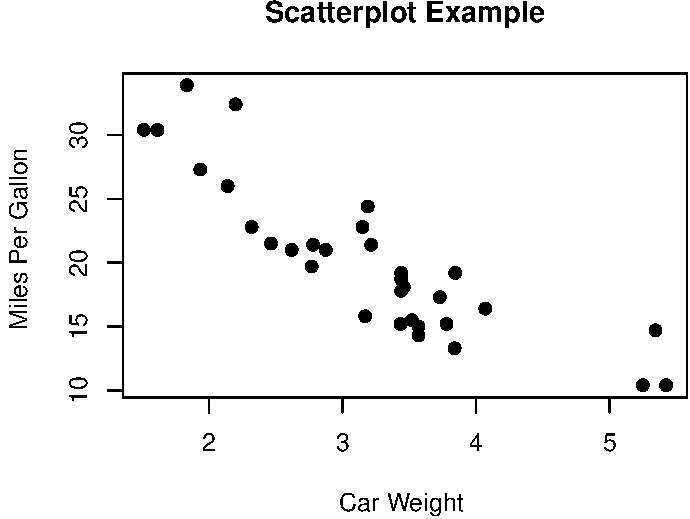
\includegraphics{index_files/figure-latex/unnamed-chunk-60-1.pdf}

\begin{itemize}
\tightlist
\item
  Basic Scatterplot Matrix
\end{itemize}

\begin{Shaded}
\begin{Highlighting}[]
\KeywordTok{pairs}\NormalTok{(~mpg+disp+drat+wt,}\DataTypeTok{data=}\NormalTok{mtcars,}
   \DataTypeTok{main=}\StringTok{"Simple Scatterplot Matrix"}\NormalTok{)}
\end{Highlighting}
\end{Shaded}

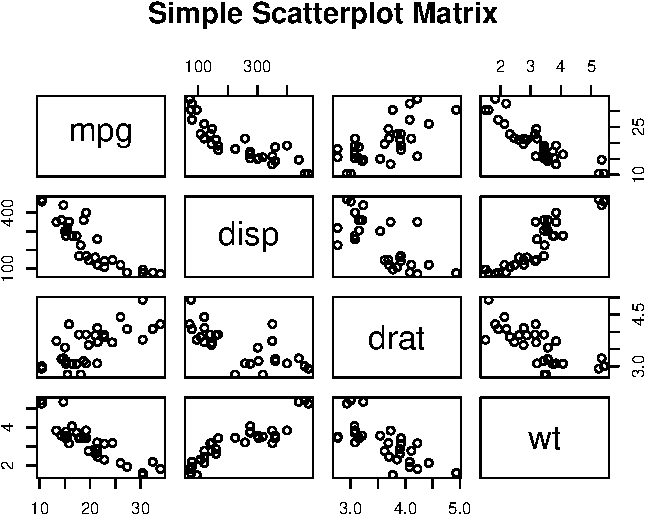
\includegraphics{index_files/figure-latex/unnamed-chunk-61-1.pdf}

\begin{itemize}
\tightlist
\item
  Barplot
\end{itemize}

\begin{Shaded}
\begin{Highlighting}[]
\NormalTok{tab <-}\StringTok{ }\KeywordTok{table}\NormalTok{(mtcars[,}\KeywordTok{c}\NormalTok{(}\StringTok{"cyl"}\NormalTok{)])}
\KeywordTok{barplot}\NormalTok{(tab)}
\end{Highlighting}
\end{Shaded}

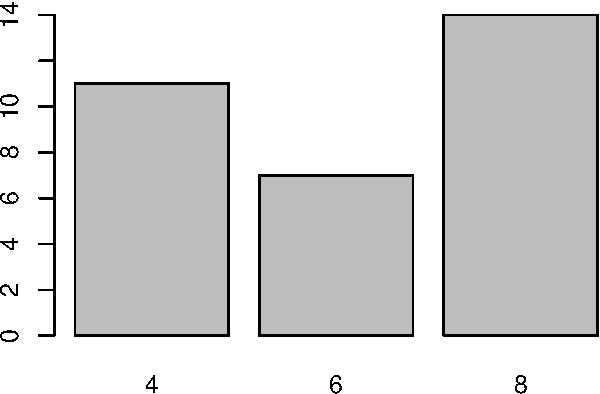
\includegraphics{index_files/figure-latex/unnamed-chunk-62-1.pdf}

\begin{itemize}
\tightlist
\item
  Piechart
\end{itemize}

\begin{Shaded}
\begin{Highlighting}[]
\KeywordTok{pie}\NormalTok{(tab)}
\end{Highlighting}
\end{Shaded}

\begin{center}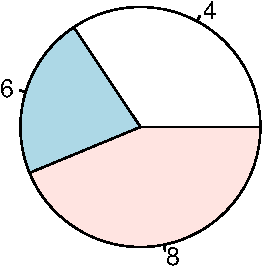
\includegraphics{index_files/figure-latex/unnamed-chunk-63-1} \end{center}

\begin{center}\rule{0.5\linewidth}{\linethickness}\end{center}

\textbf{Exercises:}

\begin{enumerate}
\def\labelenumi{\arabic{enumi}.}
\tightlist
\item
  The data.frame \texttt{VADeaths} contains the death rates per 1000 in
  Virginia (US) in 1940
\end{enumerate}

\begin{itemize}
\tightlist
\item
  The death rates are measured per 1000 population per year. They are
  cross-classified by age group (rows) and population group (columns).
  The age groups are: 50-54, 55-59, 60-64, 65-69, 70-74 and the
  population groups are Rural/Male, Rural/Female, Urban/Male and
  Urban/Female.
\end{itemize}

\begin{Shaded}
\begin{Highlighting}[]
\KeywordTok{data}\NormalTok{(VADeaths)}
\NormalTok{VADeaths}
\end{Highlighting}
\end{Shaded}

\begin{verbatim}
##       Rural Male Rural Female Urban Male Urban Female
## 50-54       11.7          8.7       15.4          8.4
## 55-59       18.1         11.7       24.3         13.6
## 60-64       26.9         20.3       37.0         19.3
## 65-69       41.0         30.9       54.6         35.1
## 70-74       66.0         54.3       71.1         50.0
\end{verbatim}

\begin{itemize}
\item
  Compute the mean for each age group.

  \begin{itemize}
  \tightlist
  \item
    \textbf{Result:}
  \end{itemize}
\end{itemize}

\begin{verbatim}
##  50-54  55-59  60-64  65-69  70-74 
## 11.050 16.925 25.875 40.400 60.350
\end{verbatim}

\begin{itemize}
\item
  Compute the mean for each population group.

  \begin{itemize}
  \tightlist
  \item
    \textbf{Result:}
  \end{itemize}
\end{itemize}

\begin{verbatim}
##   Rural Male Rural Female   Urban Male Urban Female 
##        32.74        25.18        40.48        25.28
\end{verbatim}

\begin{enumerate}
\def\labelenumi{\arabic{enumi}.}
\setcounter{enumi}{1}
\tightlist
\item
  The \texttt{data.frame} \texttt{rainforest} contains several variables
  from different \texttt{species}
\end{enumerate}

\begin{Shaded}
\begin{Highlighting}[]
\KeywordTok{library}\NormalTok{(DAAG)}
\NormalTok{rainforest}
\end{Highlighting}
\end{Shaded}

\begin{itemize}
\item
  Create a table of counts for each \texttt{species} and make a graphic
  with the results.

  \begin{itemize}
  \tightlist
  \item
    \textbf{Result:}
  \end{itemize}
\end{itemize}

\begin{verbatim}
## 
## Acacia mabellae      C. fraseri  Acmena smithii   B. myrtifolia 
##              16              12              26              11
\end{verbatim}

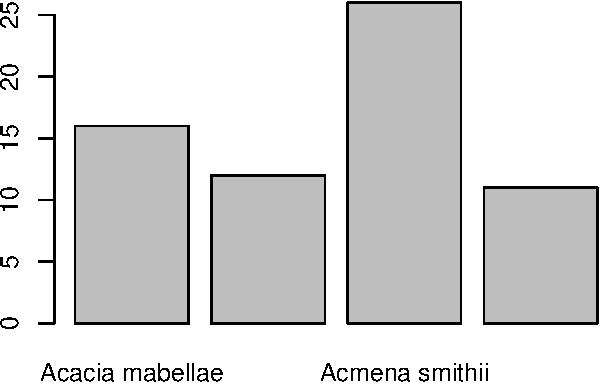
\includegraphics{index_files/figure-latex/unnamed-chunk-68-1.pdf}

\begin{enumerate}
\def\labelenumi{\arabic{enumi}.}
\setcounter{enumi}{2}
\tightlist
\item
  The \texttt{Acmena} \texttt{data.frame} is created from
  \texttt{rainforest} using the function \texttt{subset}.
\end{enumerate}

\begin{itemize}
\tightlist
\item
  Plot the relationship between the wood biomass (\texttt{wood}) and the
  diameter of the breast height (\texttt{dbh}). Use also a logarithm
  scale.
\end{itemize}

\begin{Shaded}
\begin{Highlighting}[]
\NormalTok{Acmena <-}\StringTok{ }\KeywordTok{subset}\NormalTok{(rainforest, species ==}\StringTok{ "Acmena smithii"}\NormalTok{)}
\end{Highlighting}
\end{Shaded}

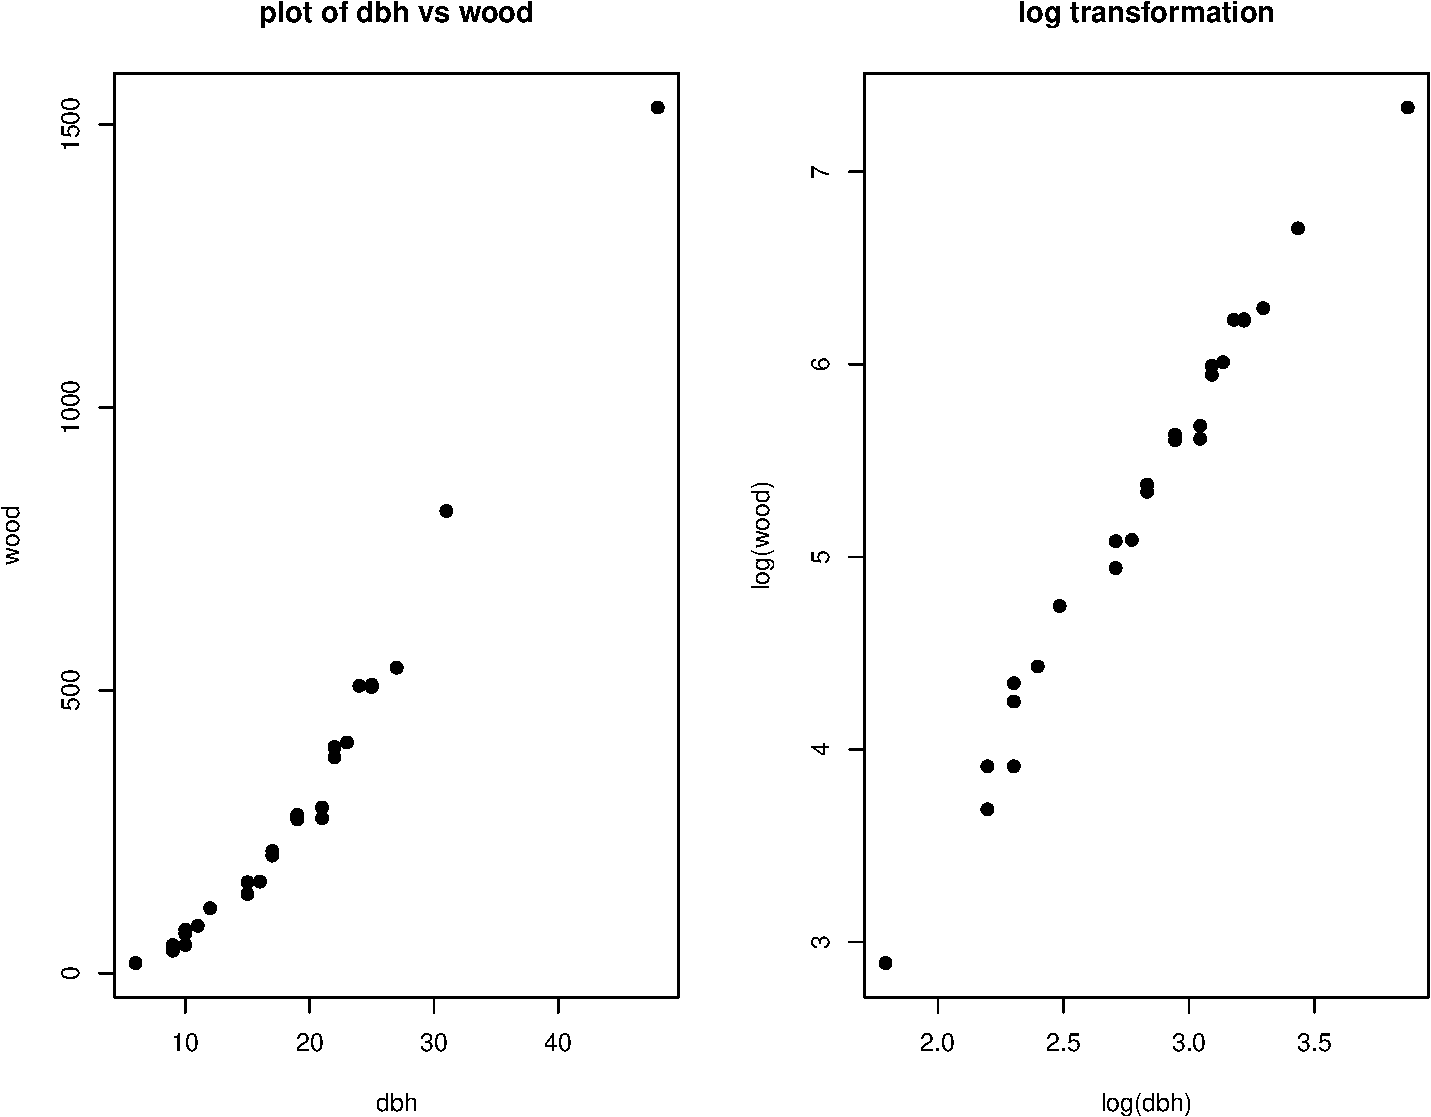
\includegraphics{index_files/figure-latex/unnamed-chunk-70-1.pdf}

\begin{itemize}
\tightlist
\item
  Compute a histogram of variable \texttt{dbh} using function
  \texttt{hist}
\end{itemize}

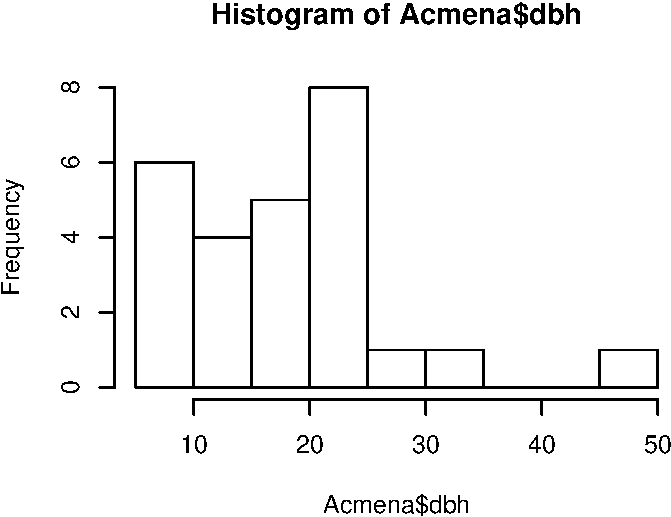
\includegraphics{index_files/figure-latex/unnamed-chunk-71-1.pdf}

\begin{enumerate}
\def\labelenumi{\arabic{enumi}.}
\setcounter{enumi}{3}
\item
  Create a vector of the positive odd integers less than 100 and remove
  the values greater than 60 and less than 80.

  \begin{itemize}
  \tightlist
  \item
    \textbf{Result:}
  \end{itemize}
\end{enumerate}

\begin{verbatim}
##  [1] 61 63 65 67 69 71 73 75 77 79
\end{verbatim}

\begin{itemize}
\tightlist
\item
  \href{http://idaejin.github.io/bcam-courses/rbasics/rbasics_sol.R}{Solutions
  here}
\end{itemize}

\begin{center}\rule{0.5\linewidth}{\linethickness}\end{center}

\subsection{Scatterplots}\label{scatterplots}

\begin{Shaded}
\begin{Highlighting}[]
\KeywordTok{library}\NormalTok{(MASS)}
\KeywordTok{data}\NormalTok{(}\StringTok{"mammals"}\NormalTok{)}
\NormalTok{?mammals}
\KeywordTok{head}\NormalTok{(mammals)}
\end{Highlighting}
\end{Shaded}

\begin{verbatim}
##                    body brain
## Arctic fox        3.385  44.5
## Owl monkey        0.480  15.5
## Mountain beaver   1.350   8.1
## Cow             465.000 423.0
## Grey wolf        36.330 119.5
## Goat             27.660 115.0
\end{verbatim}

\begin{Shaded}
\begin{Highlighting}[]
\KeywordTok{attach}\NormalTok{(mammals)}
\NormalTok{species <-}\StringTok{ }\KeywordTok{row.names}\NormalTok{(mammals)}
\NormalTok{x <-}\StringTok{ }\NormalTok{body}
\NormalTok{y <-}\StringTok{ }\NormalTok{brain}
\end{Highlighting}
\end{Shaded}

\begin{Shaded}
\begin{Highlighting}[]
\KeywordTok{library}\NormalTok{(calibrate)}
\CommentTok{# scatterplot}
\KeywordTok{plot}\NormalTok{(x,y, }\DataTypeTok{xlab =} \StringTok{"body weight in kgr"}\NormalTok{, }\DataTypeTok{ylab =} \StringTok{"brain weight in gr"}\NormalTok{, }
     \DataTypeTok{main=}\StringTok{"Body vs Brain weight }\CharTok{\textbackslash{}n}\StringTok{ for 62 Species of Land Mammals"}\NormalTok{)}
\KeywordTok{textxy}\NormalTok{(x,y,}\DataTypeTok{labs=}\NormalTok{species,}\DataTypeTok{col =} \StringTok{"blue"}\NormalTok{,}\DataTypeTok{cex=}\FloatTok{0.85}\NormalTok{) }
\end{Highlighting}
\end{Shaded}

\begin{center}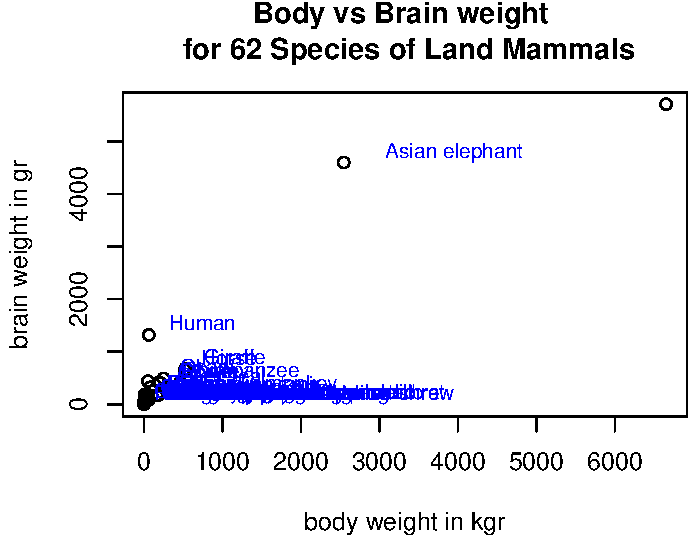
\includegraphics{index_files/figure-latex/unnamed-chunk-74-1} \end{center}

Identify a point in the scatterplot

\begin{Shaded}
\begin{Highlighting}[]
\KeywordTok{identify}\NormalTok{(x,y,species)}
\end{Highlighting}
\end{Shaded}

Plot in the log scale

\begin{Shaded}
\begin{Highlighting}[]
\KeywordTok{plot}\NormalTok{(}\KeywordTok{log}\NormalTok{(x),}\KeywordTok{log}\NormalTok{(y), }\DataTypeTok{xlab =} \StringTok{"log body weight in kgr"}\NormalTok{, }\DataTypeTok{ylab =} \StringTok{"log brain weight in gr"}\NormalTok{, }
     \DataTypeTok{main=}\StringTok{"log Body vs log Brain weight }\CharTok{\textbackslash{}n}\StringTok{ for 62 Species of Land Mammals"}\NormalTok{)}
\KeywordTok{textxy}\NormalTok{(}\KeywordTok{log}\NormalTok{(x),}\KeywordTok{log}\NormalTok{(y),}\DataTypeTok{labs=}\NormalTok{species,}\DataTypeTok{col =} \StringTok{"blue"}\NormalTok{,}\DataTypeTok{cex=}\FloatTok{0.85}\NormalTok{) }
\end{Highlighting}
\end{Shaded}

\begin{center}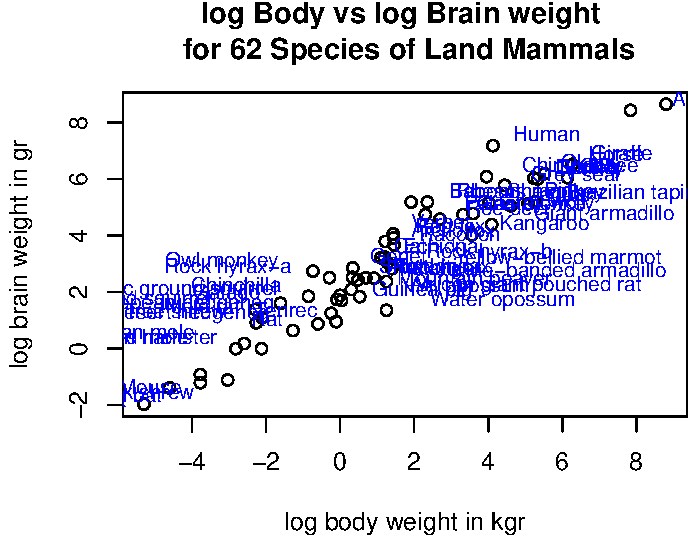
\includegraphics{index_files/figure-latex/unnamed-chunk-76-1} \end{center}

Identify a point in the log scale scatterplot

\begin{Shaded}
\begin{Highlighting}[]
\KeywordTok{identify}\NormalTok{(}\KeywordTok{log}\NormalTok{(x),}\KeywordTok{log}\NormalTok{(y),species)}
\end{Highlighting}
\end{Shaded}

\subsection{More plotting options}\label{more-plotting-options}

\textbf{Multiple Data Sets on One Plot}

One common task is to plot multiple data sets on the same plot. In many
situations the way to do this is to create the initial plot and then add
additional information to the plot. For example, to plot bivariate data
the \texttt{plot} command is used to initialize and create the plot. The
\texttt{points} command can then be used to add additional data sets to
the plot.

\begin{Shaded}
\begin{Highlighting}[]
 \NormalTok{x <-}\StringTok{ }\KeywordTok{rnorm}\NormalTok{(}\DecValTok{10}\NormalTok{,}\DataTypeTok{sd=}\DecValTok{5}\NormalTok{,}\DataTypeTok{mean=}\DecValTok{20}\NormalTok{)}
 \NormalTok{y <-}\StringTok{ }\FloatTok{2.5}\NormalTok{*x -}\StringTok{ }\FloatTok{1.0} \NormalTok{+}\StringTok{ }\KeywordTok{rnorm}\NormalTok{(}\DecValTok{10}\NormalTok{,}\DataTypeTok{sd=}\DecValTok{9}\NormalTok{,}\DataTypeTok{mean=}\DecValTok{0}\NormalTok{)}
 \KeywordTok{cor}\NormalTok{(x,y)}
\end{Highlighting}
\end{Shaded}

\begin{verbatim}
## [1] 0.878009
\end{verbatim}

\begin{Shaded}
\begin{Highlighting}[]
 \KeywordTok{plot}\NormalTok{(x,y,}\DataTypeTok{xlab=}\StringTok{"Independent"}\NormalTok{,}\DataTypeTok{ylab=}\StringTok{"Dependent"}\NormalTok{,}\DataTypeTok{main=}\StringTok{"Random plot"}\NormalTok{)}
 \NormalTok{x1 <-}\StringTok{ }\KeywordTok{runif}\NormalTok{(}\DecValTok{8}\NormalTok{,}\DecValTok{15}\NormalTok{,}\DecValTok{25}\NormalTok{)}
 \NormalTok{y1 <-}\StringTok{ }\FloatTok{2.5}\NormalTok{*x1 -}\StringTok{ }\FloatTok{1.0} \NormalTok{+}\StringTok{ }\KeywordTok{runif}\NormalTok{(}\DecValTok{8}\NormalTok{,-}\DecValTok{6}\NormalTok{,}\DecValTok{6}\NormalTok{)}
 \KeywordTok{points}\NormalTok{(x1,y1,}\DataTypeTok{col=}\DecValTok{2}\NormalTok{)}
\end{Highlighting}
\end{Shaded}

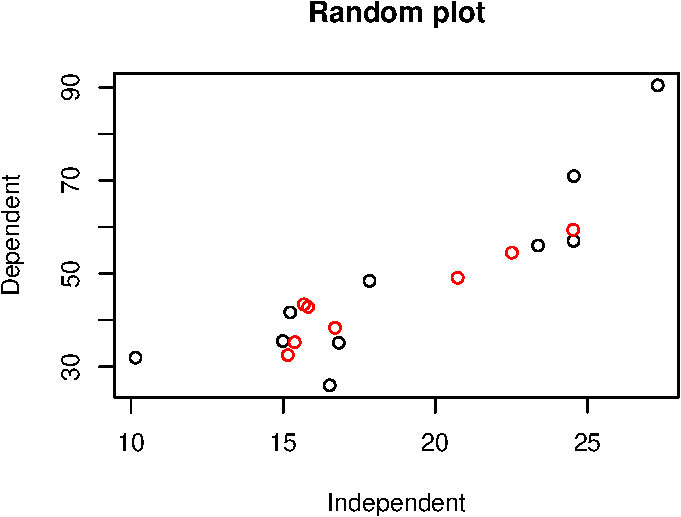
\includegraphics{index_files/figure-latex/unnamed-chunk-78-1.pdf}

with legend and \((x_2,y_2)\) points:

\begin{Shaded}
\begin{Highlighting}[]
\NormalTok{x2 <-}\StringTok{ }\KeywordTok{runif}\NormalTok{(}\DecValTok{8}\NormalTok{,}\DecValTok{15}\NormalTok{,}\DecValTok{25}\NormalTok{)}
\NormalTok{y2 <-}\StringTok{ }\FloatTok{2.5}\NormalTok{*x2 -}\StringTok{ }\FloatTok{1.0} \NormalTok{+}\StringTok{ }\KeywordTok{runif}\NormalTok{(}\DecValTok{8}\NormalTok{,-}\DecValTok{6}\NormalTok{,}\DecValTok{6}\NormalTok{)}
 \KeywordTok{plot}\NormalTok{(x,y,}\DataTypeTok{xlab=}\StringTok{"Independent"}\NormalTok{,}\DataTypeTok{ylab=}\StringTok{"Dependent"}\NormalTok{,}\DataTypeTok{main=}\StringTok{"Random plot"}\NormalTok{)}
 \KeywordTok{points}\NormalTok{(x1,y1,}\DataTypeTok{col=}\DecValTok{2}\NormalTok{,}\DataTypeTok{pch=}\DecValTok{3}\NormalTok{)}
 \KeywordTok{points}\NormalTok{(x2,y2,}\DataTypeTok{col=}\DecValTok{4}\NormalTok{,}\DataTypeTok{pch=}\DecValTok{5}\NormalTok{)}
 \KeywordTok{legend}\NormalTok{(}\StringTok{"topleft"}\NormalTok{,}\KeywordTok{c}\NormalTok{(}\StringTok{"Original"}\NormalTok{,}\StringTok{"one"}\NormalTok{,}\StringTok{"two"}\NormalTok{),}\DataTypeTok{col=}\KeywordTok{c}\NormalTok{(}\DecValTok{1}\NormalTok{,}\DecValTok{2}\NormalTok{,}\DecValTok{4}\NormalTok{),}\DataTypeTok{pch=}\KeywordTok{c}\NormalTok{(}\DecValTok{1}\NormalTok{,}\DecValTok{3}\NormalTok{,}\DecValTok{5}\NormalTok{))}
\end{Highlighting}
\end{Shaded}

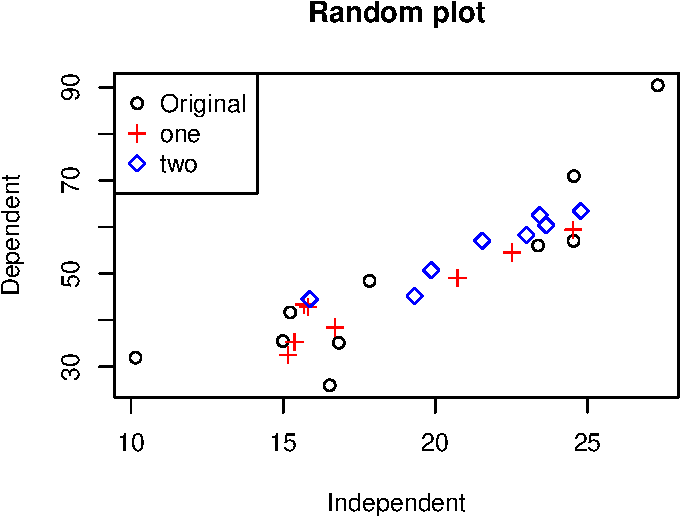
\includegraphics{index_files/figure-latex/unnamed-chunk-79-1.pdf}

\textbf{Errors bars:}

\begin{Shaded}
\begin{Highlighting}[]
\KeywordTok{plot}\NormalTok{(x,y,}\DataTypeTok{xlab=}\StringTok{"Independent"}\NormalTok{,}\DataTypeTok{ylab=}\StringTok{"Dependent"}\NormalTok{,}\DataTypeTok{main=}\StringTok{"Random plot"}\NormalTok{,}\DataTypeTok{ylim=}\KeywordTok{c}\NormalTok{(}\DecValTok{20}\NormalTok{,}\DecValTok{90}\NormalTok{))}
\NormalTok{xHigh <-}\StringTok{ }\NormalTok{x}
\NormalTok{yHigh <-}\StringTok{ }\NormalTok{y +}\StringTok{ }\KeywordTok{abs}\NormalTok{(}\KeywordTok{rnorm}\NormalTok{(}\DecValTok{10}\NormalTok{,}\DataTypeTok{sd=}\FloatTok{3.5}\NormalTok{))}
\NormalTok{xLow <-}\StringTok{ }\NormalTok{x}
\NormalTok{yLow <-}\StringTok{ }\NormalTok{y -}\StringTok{ }\KeywordTok{abs}\NormalTok{(}\KeywordTok{rnorm}\NormalTok{(}\DecValTok{10}\NormalTok{,}\DataTypeTok{sd=}\FloatTok{3.1}\NormalTok{))}
\KeywordTok{arrows}\NormalTok{(xHigh,yHigh,xLow,yLow,}\DataTypeTok{col=}\DecValTok{2}\NormalTok{,}\DataTypeTok{angle=}\DecValTok{90}\NormalTok{,}\DataTypeTok{length=}\FloatTok{0.1}\NormalTok{,}\DataTypeTok{code=}\DecValTok{3}\NormalTok{)}
\end{Highlighting}
\end{Shaded}

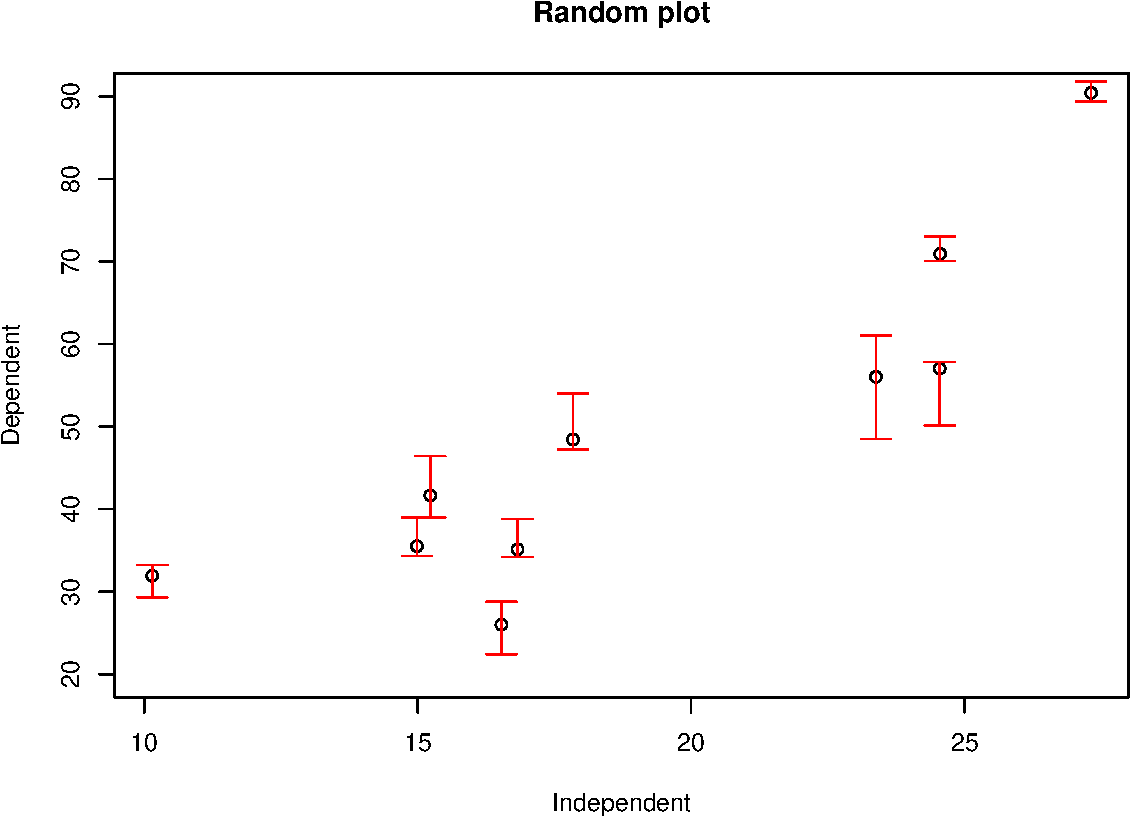
\includegraphics{index_files/figure-latex/unnamed-chunk-80-1.pdf}

\begin{Shaded}
\begin{Highlighting}[]
\KeywordTok{plot}\NormalTok{(}\DecValTok{1}\NormalTok{:}\DecValTok{20}\NormalTok{,}\DecValTok{0}\NormalTok{*(}\DecValTok{1}\NormalTok{:}\DecValTok{20}\NormalTok{),}\DataTypeTok{pch=}\DecValTok{1}\NormalTok{:}\DecValTok{20}\NormalTok{,}\DataTypeTok{cex=}\DecValTok{2}\NormalTok{)}
\end{Highlighting}
\end{Shaded}

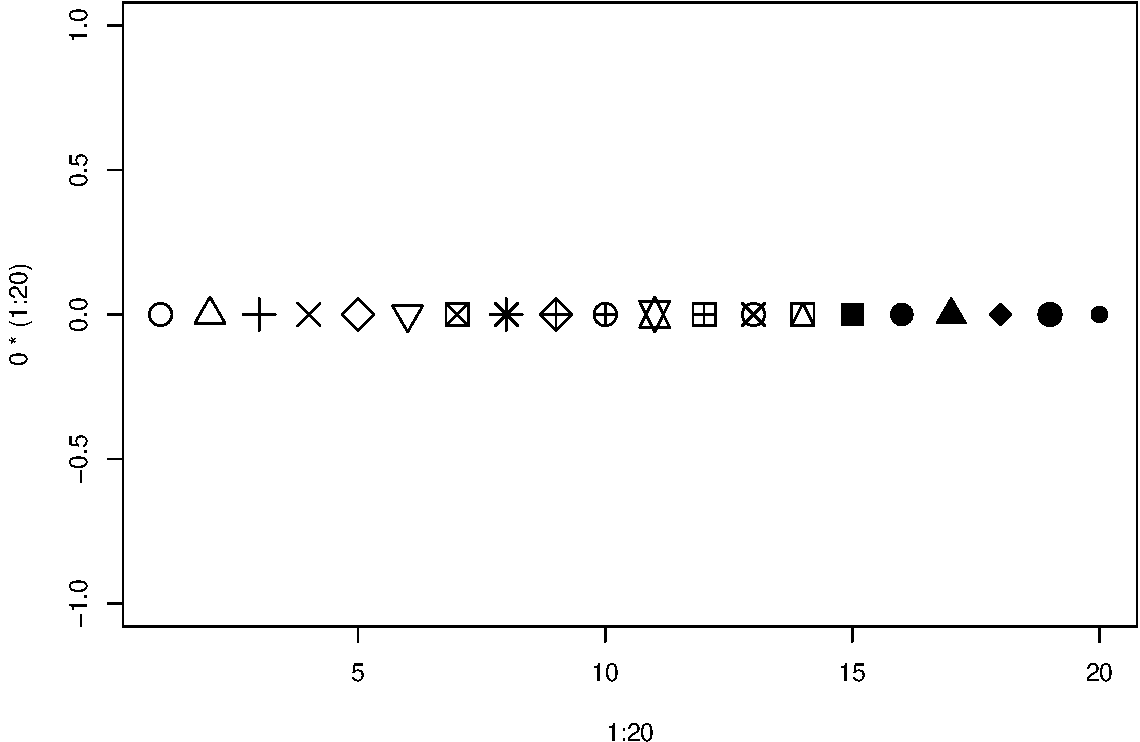
\includegraphics{index_files/figure-latex/unnamed-chunk-81-1.pdf}

\textbf{Multiple Graphs on One Image:}

\begin{Shaded}
\begin{Highlighting}[]
 \KeywordTok{par}\NormalTok{(}\DataTypeTok{mfrow=}\KeywordTok{c}\NormalTok{(}\DecValTok{2}\NormalTok{,}\DecValTok{3}\NormalTok{))}
 \KeywordTok{boxplot}\NormalTok{(}\KeywordTok{rnorm}\NormalTok{(}\DecValTok{100}\NormalTok{),}\DataTypeTok{main=}\StringTok{"first plot"}\NormalTok{)}
 \KeywordTok{boxplot}\NormalTok{(}\KeywordTok{rgamma}\NormalTok{(}\DecValTok{100}\NormalTok{,}\DecValTok{2}\NormalTok{),}\DataTypeTok{main=}\StringTok{"second plot"}\NormalTok{, }\DataTypeTok{horizontal=}\OtherTok{TRUE}\NormalTok{,}\DataTypeTok{col=}\StringTok{"bisque"}\NormalTok{)}
 \KeywordTok{plot}\NormalTok{(}\KeywordTok{rnorm}\NormalTok{(}\DecValTok{100}\NormalTok{),}\DataTypeTok{xlab=}\StringTok{"third plot"}\NormalTok{,}
      \DataTypeTok{ylab=}\StringTok{"y-label"}\NormalTok{,}\DataTypeTok{main=}\StringTok{"x-label"}\NormalTok{)}
 \KeywordTok{hist}\NormalTok{(}\KeywordTok{rnorm}\NormalTok{(}\DecValTok{100}\NormalTok{),}\DataTypeTok{main=}\StringTok{"fourth plot"}\NormalTok{,}\DataTypeTok{col=}\StringTok{"lightgrey"}\NormalTok{)}
 \KeywordTok{hist}\NormalTok{(}\KeywordTok{rexp}\NormalTok{(}\DecValTok{100}\NormalTok{),}\DataTypeTok{main=}\StringTok{"fifth plot"}\NormalTok{,}\DataTypeTok{col=}\StringTok{"blue"}\NormalTok{)}
 \KeywordTok{plot}\NormalTok{(}\KeywordTok{rnorm}\NormalTok{(}\DecValTok{100}\NormalTok{),}\KeywordTok{rexp}\NormalTok{(}\DecValTok{100}\NormalTok{),}\DataTypeTok{main=}\StringTok{"sixth plot"}\NormalTok{)}
\end{Highlighting}
\end{Shaded}

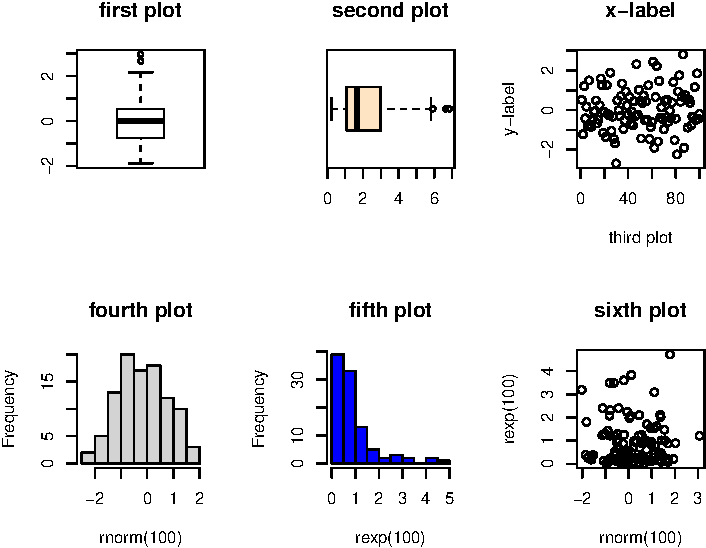
\includegraphics{index_files/figure-latex/unnamed-chunk-82-1.pdf}

\textbf{Pairwise relationships}

\begin{Shaded}
\begin{Highlighting}[]
\NormalTok{uData <-}\StringTok{ }\KeywordTok{rnorm}\NormalTok{(}\DecValTok{20}\NormalTok{)}
\NormalTok{vData <-}\StringTok{ }\KeywordTok{rnorm}\NormalTok{(}\DecValTok{20}\NormalTok{,}\DataTypeTok{mean=}\DecValTok{5}\NormalTok{)}
\NormalTok{wData <-}\StringTok{ }\NormalTok{uData +}\StringTok{ }\DecValTok{2}\NormalTok{*vData +}\StringTok{ }\KeywordTok{rnorm}\NormalTok{(}\DecValTok{20}\NormalTok{,}\DataTypeTok{sd=}\FloatTok{0.5}\NormalTok{)}
\NormalTok{xData <-}\StringTok{ }\NormalTok{-}\DecValTok{2}\NormalTok{*uData+}\KeywordTok{rnorm}\NormalTok{(}\DecValTok{20}\NormalTok{,}\DataTypeTok{sd=}\FloatTok{0.1}\NormalTok{)}
\NormalTok{yData <-}\StringTok{ }\DecValTok{3}\NormalTok{*vData+}\KeywordTok{rnorm}\NormalTok{(}\DecValTok{20}\NormalTok{,}\DataTypeTok{sd=}\FloatTok{2.5}\NormalTok{)}
\NormalTok{d <-}\StringTok{ }\KeywordTok{data.frame}\NormalTok{(}\DataTypeTok{u=}\NormalTok{uData,}\DataTypeTok{v=}\NormalTok{vData,}\DataTypeTok{w=}\NormalTok{wData,}\DataTypeTok{x=}\NormalTok{xData,}\DataTypeTok{y=}\NormalTok{yData)}
\KeywordTok{pairs}\NormalTok{(d)}
\end{Highlighting}
\end{Shaded}

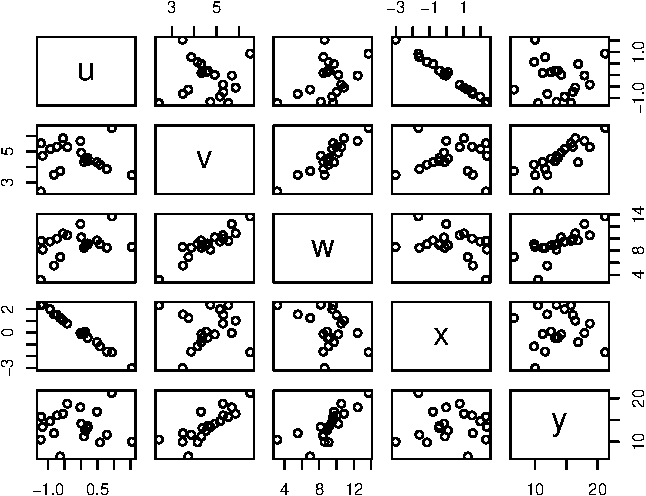
\includegraphics{index_files/figure-latex/unnamed-chunk-83-1.pdf}

\textbf{Plotting correlations}

The function \texttt{corrplot} in the \texttt{library(corrplot)}
visualizes a correlation matrix calculate with function \texttt{cor}

\begin{Shaded}
\begin{Highlighting}[]
\KeywordTok{library}\NormalTok{(corrplot)}
\NormalTok{M <-}\StringTok{ }\KeywordTok{cor}\NormalTok{(d)}
\KeywordTok{corrplot}\NormalTok{(M, }\DataTypeTok{method=}\StringTok{"circle"}\NormalTok{,}\DataTypeTok{type=}\StringTok{"upper"}\NormalTok{)}
\end{Highlighting}
\end{Shaded}

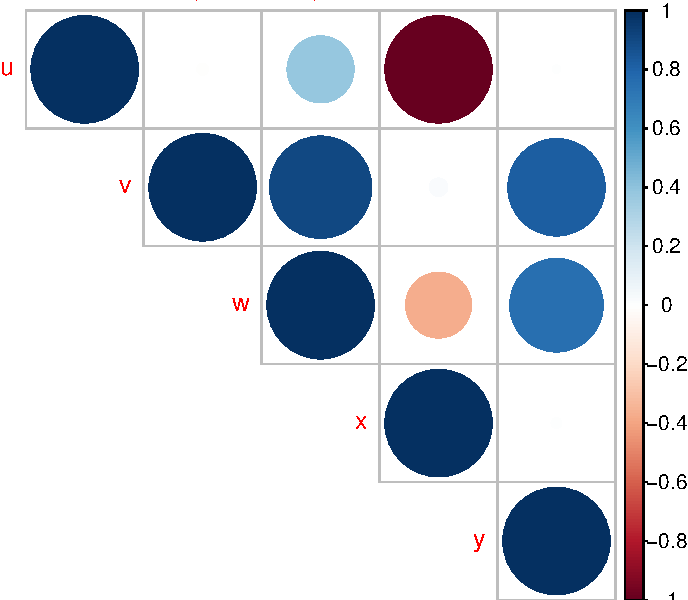
\includegraphics{index_files/figure-latex/unnamed-chunk-84-1.pdf}

\textbf{Plotting surfaces: \texttt{image}, \texttt{contour} and
\texttt{persp} plots}

\begin{Shaded}
\begin{Highlighting}[]
\NormalTok{x <-}\StringTok{ }\KeywordTok{seq}\NormalTok{(}\DecValTok{0}\NormalTok{,}\DecValTok{2}\NormalTok{*pi,}\DataTypeTok{by=}\NormalTok{pi/}\DecValTok{50}\NormalTok{)}
\NormalTok{y <-}\StringTok{ }\NormalTok{x}
\NormalTok{xg <-}\StringTok{ }\NormalTok{(x*}\DecValTok{0+1}\NormalTok{) %*%}\StringTok{ }\KeywordTok{t}\NormalTok{(y)}
\NormalTok{yg <-}\StringTok{ }\NormalTok{(x) %*%}\StringTok{ }\KeywordTok{t}\NormalTok{(y*}\DecValTok{0+1}\NormalTok{)}
\NormalTok{f <-}\StringTok{ }\KeywordTok{sin}\NormalTok{(xg*yg)}

\KeywordTok{par}\NormalTok{(}\DataTypeTok{mfrow=}\KeywordTok{c}\NormalTok{(}\DecValTok{2}\NormalTok{,}\DecValTok{2}\NormalTok{))}
\KeywordTok{image}\NormalTok{(x,y,f)}
\KeywordTok{contour}\NormalTok{(x,y,f)}
\KeywordTok{contour}\NormalTok{(x,y,f,}\DataTypeTok{nlevels=}\DecValTok{4}\NormalTok{)}
\KeywordTok{image}\NormalTok{(x,y,f,}\DataTypeTok{col=}\KeywordTok{grey.colors}\NormalTok{(}\DecValTok{100}\NormalTok{))}
\KeywordTok{contour}\NormalTok{(x,y,f,}\DataTypeTok{nlevels=}\DecValTok{4}\NormalTok{,}\DataTypeTok{add=}\OtherTok{TRUE}\NormalTok{,}\DataTypeTok{col=}\StringTok{"red"}\NormalTok{)}
\end{Highlighting}
\end{Shaded}

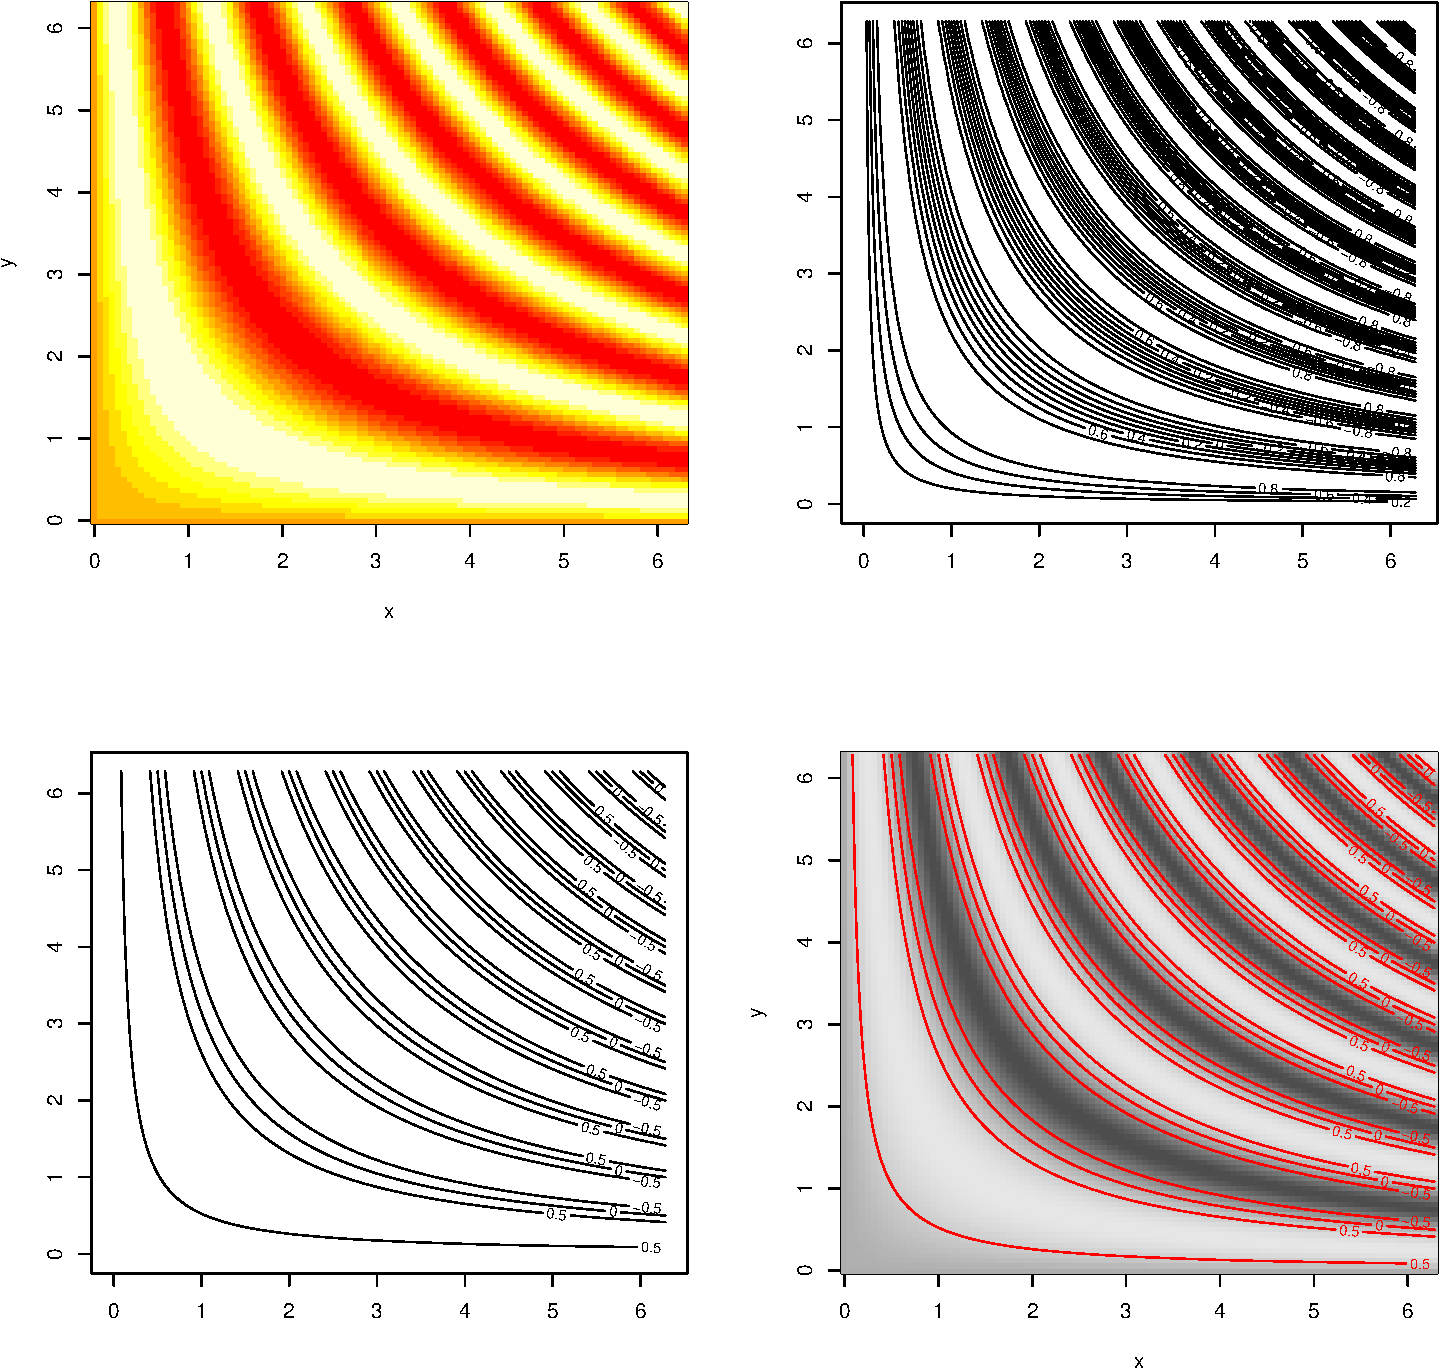
\includegraphics{index_files/figure-latex/unnamed-chunk-85-1.pdf}

Similarly, one can use \texttt{persp} plot

\begin{Shaded}
\begin{Highlighting}[]
\KeywordTok{persp}\NormalTok{(x,y,f,}\DataTypeTok{theta=}\NormalTok{-}\DecValTok{30}\NormalTok{,}\DataTypeTok{phi=}\DecValTok{55}\NormalTok{,}\DataTypeTok{col=}\StringTok{"lightgrey"}\NormalTok{,}\DataTypeTok{shade=}\NormalTok{.}\DecValTok{01}\NormalTok{)}
\end{Highlighting}
\end{Shaded}

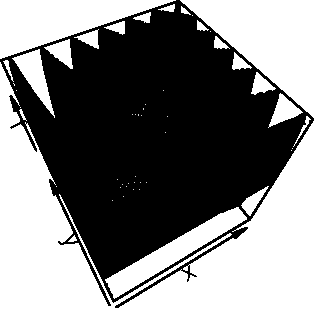
\includegraphics{index_files/figure-latex/unnamed-chunk-86-1.pdf}

\subsection{QQ-plot}\label{qq-plot}

A Q-Q plot is a plot of the quantiles of two distributions against each
other, or a plot based on estimates of the quantiles. The pattern of
points in the plot is used to compare the two distributions.

\texttt{qqnorm} is used to determine if your data is close to being
normally distributed. You cannot be sure that the data is normally
distributed, but you can rule out if it is not normally distributed.

\begin{Shaded}
\begin{Highlighting}[]
\KeywordTok{set.seed}\NormalTok{(}\DecValTok{1234}\NormalTok{)}

\KeywordTok{require}\NormalTok{(graphics)}
\NormalTok{y <-}\StringTok{ }\KeywordTok{rt}\NormalTok{(}\DecValTok{200}\NormalTok{, }\DataTypeTok{df =} \DecValTok{5}\NormalTok{)}
\KeywordTok{qqnorm}\NormalTok{(y); }
\KeywordTok{qqline}\NormalTok{(y, }\DataTypeTok{col =} \DecValTok{2}\NormalTok{)}
\end{Highlighting}
\end{Shaded}

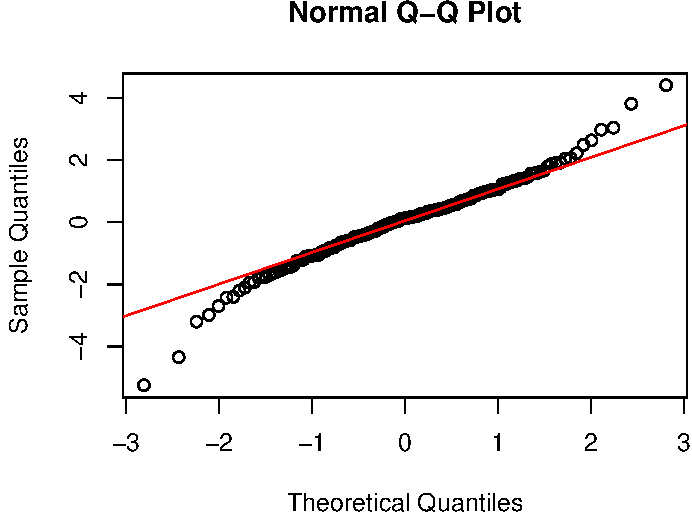
\includegraphics{index_files/figure-latex/unnamed-chunk-87-1.pdf}

\begin{Shaded}
\begin{Highlighting}[]
\NormalTok{z <-}\StringTok{ }\KeywordTok{rnorm}\NormalTok{(}\DecValTok{200}\NormalTok{,}\DataTypeTok{mean=}\DecValTok{0}\NormalTok{,}\DataTypeTok{sd=}\DecValTok{1}\NormalTok{)}
\KeywordTok{qqnorm}\NormalTok{(z)}
\KeywordTok{qqline}\NormalTok{(z, }\DataTypeTok{col =} \DecValTok{2}\NormalTok{)}
\end{Highlighting}
\end{Shaded}

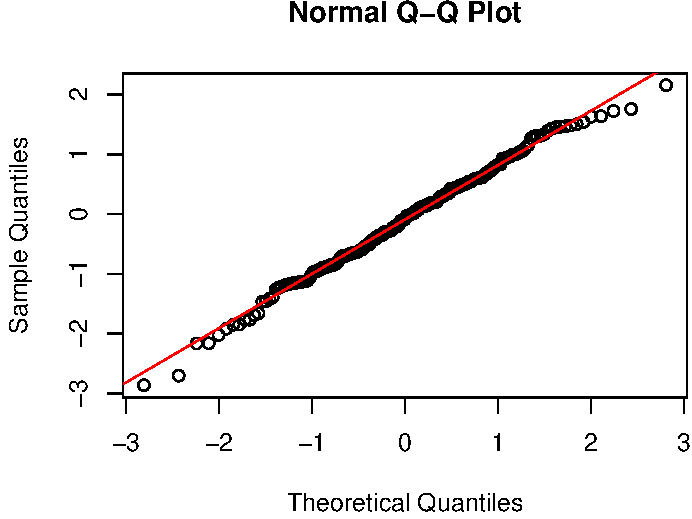
\includegraphics{index_files/figure-latex/unnamed-chunk-87-2.pdf}

To compare two distributions

\begin{Shaded}
\begin{Highlighting}[]
\KeywordTok{set.seed}\NormalTok{(}\DecValTok{1234}\NormalTok{)}
\KeywordTok{qqplot}\NormalTok{(}\KeywordTok{qchisq}\NormalTok{(}\KeywordTok{ppoints}\NormalTok{(}\DecValTok{500}\NormalTok{), }\DataTypeTok{df =} \DecValTok{3}\NormalTok{), y,}
       \DataTypeTok{main =} \KeywordTok{expression}\NormalTok{(}\StringTok{"Q-Q plot for"} \NormalTok{~}\ErrorTok{~}\StringTok{ }\NormalTok{\{chi^}\DecValTok{2}\NormalTok{\}[nu ==}\StringTok{ }\DecValTok{3}\NormalTok{]))}
\KeywordTok{qqline}\NormalTok{(y, }\DataTypeTok{distribution =} \NormalTok{function(p) }\KeywordTok{qchisq}\NormalTok{(p, }\DataTypeTok{df =} \DecValTok{3}\NormalTok{),}
       \DataTypeTok{prob =} \KeywordTok{c}\NormalTok{(}\FloatTok{0.1}\NormalTok{, }\FloatTok{0.6}\NormalTok{), }\DataTypeTok{col =} \DecValTok{2}\NormalTok{)}
\end{Highlighting}
\end{Shaded}

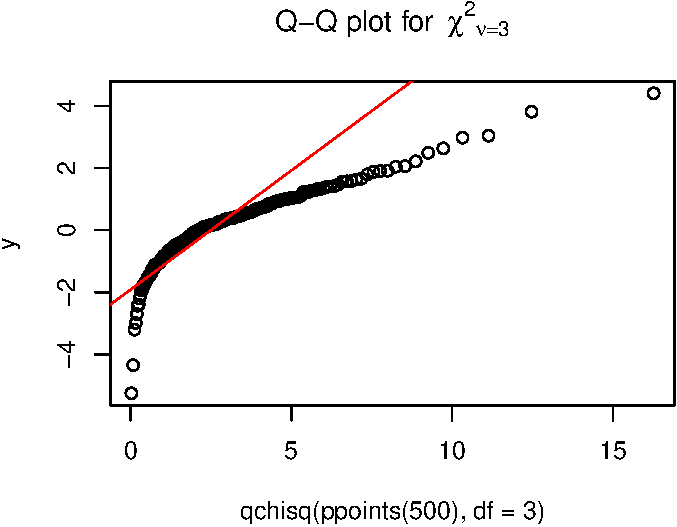
\includegraphics{index_files/figure-latex/unnamed-chunk-88-1.pdf} If the
two distributions being compared are identical, the Q-Q plot follows the
\(45º\) line y = x.

\subsection{Tables and
Cross-classification}\label{tables-and-cross-classification}

\begin{Shaded}
\begin{Highlighting}[]
\KeywordTok{library}\NormalTok{(MASS)}
\KeywordTok{data}\NormalTok{(quine)}
\NormalTok{?quine}
\KeywordTok{attach}\NormalTok{(quine)}
\KeywordTok{table}\NormalTok{(Sex)}
\end{Highlighting}
\end{Shaded}

\begin{verbatim}
## Sex
##  F  M 
## 80 66
\end{verbatim}

\begin{Shaded}
\begin{Highlighting}[]
\KeywordTok{table}\NormalTok{(Sex,Age)}
\end{Highlighting}
\end{Shaded}

\begin{verbatim}
##    Age
## Sex F0 F1 F2 F3
##   F 10 32 19 19
##   M 17 14 21 14
\end{verbatim}

\begin{Shaded}
\begin{Highlighting}[]
\CommentTok{# or xtabs}
\KeywordTok{xtabs}\NormalTok{(~Sex+Age,}\DataTypeTok{data=}\NormalTok{quine)}
\end{Highlighting}
\end{Shaded}

\begin{verbatim}
##    Age
## Sex F0 F1 F2 F3
##   F 10 32 19 19
##   M 17 14 21 14
\end{verbatim}

\begin{Shaded}
\begin{Highlighting}[]
\KeywordTok{xtabs}\NormalTok{(~Sex+Age+Eth,}\DataTypeTok{data=}\NormalTok{quine)}
\end{Highlighting}
\end{Shaded}

\begin{verbatim}
## , , Eth = A
## 
##    Age
## Sex F0 F1 F2 F3
##   F  5 15  9  9
##   M  8  5 11  7
## 
## , , Eth = N
## 
##    Age
## Sex F0 F1 F2 F3
##   F  5 17 10 10
##   M  9  9 10  7
\end{verbatim}

\subsection{Calculation of
cross-classifications}\label{calculation-of-cross-classifications}

\begin{Shaded}
\begin{Highlighting}[]
\KeywordTok{tapply}\NormalTok{(Days,Age,mean)}
\end{Highlighting}
\end{Shaded}

\begin{verbatim}
##       F0       F1       F2       F3 
## 14.85185 11.15217 21.05000 19.60606
\end{verbatim}

\begin{Shaded}
\begin{Highlighting}[]
\KeywordTok{tapply}\NormalTok{(Days,}\KeywordTok{list}\NormalTok{(Sex,Age),mean)}
\end{Highlighting}
\end{Shaded}

\begin{verbatim}
##         F0       F1       F2       F3
## F 18.70000 12.96875 18.42105 14.00000
## M 12.58824  7.00000 23.42857 27.21429
\end{verbatim}

\begin{Shaded}
\begin{Highlighting}[]
\KeywordTok{tapply}\NormalTok{(Days,}\KeywordTok{list}\NormalTok{(Sex,Age),function(x) }\KeywordTok{sqrt}\NormalTok{(}\KeywordTok{var}\NormalTok{(x)/}\KeywordTok{length}\NormalTok{(x)))}
\end{Highlighting}
\end{Shaded}

\begin{verbatim}
##         F0       F1       F2       F3
## F 4.208589 2.329892 5.299959 2.940939
## M 3.768151 1.418093 3.766122 4.569582
\end{verbatim}

\subsection{Qualitative data}\label{qualitative-data}

A data sample is called qualitative, also known as categorical, if its
values belong to a collection of known defined non-overlapping classes.
Common examples include student letter grade (A, B, C, D or F),
commercial bond rating (AAA, AAB, \ldots{}) and consumer clothing shoe
sizes (1, 2, 3, \ldots{}).

Let us consider some artificial data consisting of the
\texttt{treatment} and \texttt{improvement} of patients with rheumatoid
arthritis.

\begin{Shaded}
\begin{Highlighting}[]
\NormalTok{treatment <-}\StringTok{ }\KeywordTok{factor}\NormalTok{(}\KeywordTok{rep}\NormalTok{(}\KeywordTok{c}\NormalTok{(}\DecValTok{1}\NormalTok{, }\DecValTok{2}\NormalTok{), }\KeywordTok{c}\NormalTok{(}\DecValTok{43}\NormalTok{, }\DecValTok{41}\NormalTok{)), }\DataTypeTok{levels =} \KeywordTok{c}\NormalTok{(}\DecValTok{1}\NormalTok{, }\DecValTok{2}\NormalTok{),}
                    \DataTypeTok{labels =} \KeywordTok{c}\NormalTok{(}\StringTok{"placebo"}\NormalTok{, }\StringTok{"treated"}\NormalTok{))}
\NormalTok{improved <-}\StringTok{ }\KeywordTok{factor}\NormalTok{(}\KeywordTok{rep}\NormalTok{(}\KeywordTok{c}\NormalTok{(}\DecValTok{1}\NormalTok{, }\DecValTok{2}\NormalTok{, }\DecValTok{3}\NormalTok{, }\DecValTok{1}\NormalTok{, }\DecValTok{2}\NormalTok{, }\DecValTok{3}\NormalTok{), }\KeywordTok{c}\NormalTok{(}\DecValTok{29}\NormalTok{, }\DecValTok{7}\NormalTok{, }\DecValTok{7}\NormalTok{, }\DecValTok{13}\NormalTok{, }\DecValTok{7}\NormalTok{, }\DecValTok{21}\NormalTok{)),}
                   \DataTypeTok{levels =} \KeywordTok{c}\NormalTok{(}\DecValTok{1}\NormalTok{, }\DecValTok{2}\NormalTok{, }\DecValTok{3}\NormalTok{),}
                   \DataTypeTok{labels =} \KeywordTok{c}\NormalTok{(}\StringTok{"none"}\NormalTok{, }\StringTok{"some"}\NormalTok{, }\StringTok{"marked"}\NormalTok{))}
\end{Highlighting}
\end{Shaded}

We can compute a cross-classification table

\begin{Shaded}
\begin{Highlighting}[]
\KeywordTok{xtabs}\NormalTok{(~treatment+improved)}
\end{Highlighting}
\end{Shaded}

\begin{verbatim}
##          improved
## treatment none some marked
##   placebo   29    7      7
##   treated   13    7     21
\end{verbatim}

Graphically,

\begin{Shaded}
\begin{Highlighting}[]
\KeywordTok{spineplot}\NormalTok{(improved ~}\StringTok{ }\NormalTok{treatment)}
\end{Highlighting}
\end{Shaded}

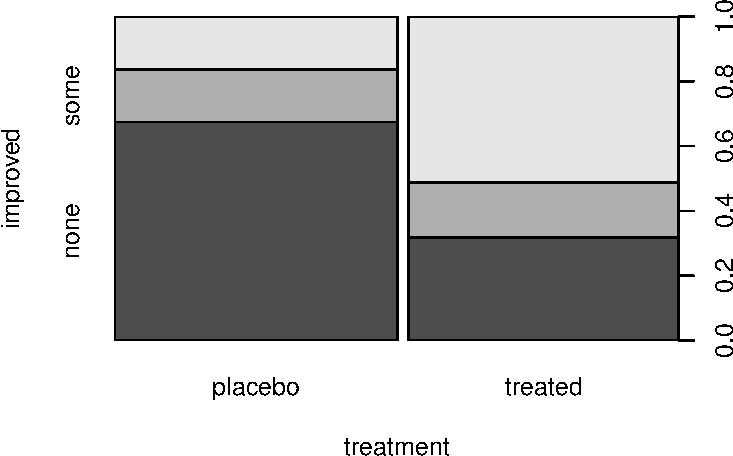
\includegraphics{index_files/figure-latex/unnamed-chunk-95-1.pdf}

The \texttt{R} dataset \texttt{UCBAdmissions} contains aggregated data
on applicants to graduate school at Berkeley for the six largest
departments in 1973 classified by admission and sex.

\begin{Shaded}
\begin{Highlighting}[]
\KeywordTok{data}\NormalTok{(}\StringTok{"UCBAdmissions"}\NormalTok{)}
\NormalTok{?UCBAdmissions}
\KeywordTok{apply}\NormalTok{(UCBAdmissions, }\KeywordTok{c}\NormalTok{(}\DecValTok{2}\NormalTok{,}\DecValTok{1}\NormalTok{), sum)}
\end{Highlighting}
\end{Shaded}

\begin{verbatim}
##         Admit
## Gender   Admitted Rejected
##   Male       1198     1493
##   Female      557     1278
\end{verbatim}

\begin{Shaded}
\begin{Highlighting}[]
\KeywordTok{prop.table}\NormalTok{(}\KeywordTok{apply}\NormalTok{(UCBAdmissions, }\KeywordTok{c}\NormalTok{(}\DecValTok{2}\NormalTok{,}\DecValTok{1}\NormalTok{), sum))}
\end{Highlighting}
\end{Shaded}

\begin{verbatim}
##         Admit
## Gender    Admitted  Rejected
##   Male   0.2646929 0.3298719
##   Female 0.1230667 0.2823685
\end{verbatim}

\begin{Shaded}
\begin{Highlighting}[]
\KeywordTok{ftable}\NormalTok{(UCBAdmissions)}
\end{Highlighting}
\end{Shaded}

\begin{verbatim}
##                 Dept   A   B   C   D   E   F
## Admit    Gender                             
## Admitted Male        512 353 120 138  53  22
##          Female       89  17 202 131  94  24
## Rejected Male        313 207 205 279 138 351
##          Female       19   8 391 244 299 317
\end{verbatim}

The same but with a more readable format can be obtained using
\texttt{ftable}

\begin{Shaded}
\begin{Highlighting}[]
\KeywordTok{ftable}\NormalTok{(}\KeywordTok{round}\NormalTok{(}\KeywordTok{prop.table}\NormalTok{(UCBAdmissions), }\DecValTok{3}\NormalTok{),}
       \DataTypeTok{row.vars=}\StringTok{"Dept"}\NormalTok{, }\DataTypeTok{col.vars =} \KeywordTok{c}\NormalTok{(}\StringTok{"Gender"}\NormalTok{, }\StringTok{"Admit"}\NormalTok{))}
\end{Highlighting}
\end{Shaded}

\begin{verbatim}
##      Gender     Male            Female         
##      Admit  Admitted Rejected Admitted Rejected
## Dept                                           
## A              0.113    0.069    0.020    0.004
## B              0.078    0.046    0.004    0.002
## C              0.027    0.045    0.045    0.086
## D              0.030    0.062    0.029    0.054
## E              0.012    0.030    0.021    0.066
## F              0.005    0.078    0.005    0.070
\end{verbatim}

More interesting are the proportions admitted for each \texttt{Gender}
by \texttt{Dept} combination (dimensions 2 and 3 of the array). Notice
that \texttt{male} and \texttt{female} admission rates are about the
same in all departments, except ``A'', where female admission rates are
higher.

\begin{Shaded}
\begin{Highlighting}[]
\CommentTok{# prop.table(UCBAdmissions, c(2,3))}
\KeywordTok{ftable}\NormalTok{(}\KeywordTok{round}\NormalTok{(}\KeywordTok{prop.table}\NormalTok{(UCBAdmissions, }\KeywordTok{c}\NormalTok{(}\DecValTok{2}\NormalTok{,}\DecValTok{3}\NormalTok{)), }\DecValTok{2}\NormalTok{),}
       \DataTypeTok{row.vars=}\StringTok{"Dept"}\NormalTok{, }\DataTypeTok{col.vars =} \KeywordTok{c}\NormalTok{(}\StringTok{"Gender"}\NormalTok{, }\StringTok{"Admit"}\NormalTok{))}
\end{Highlighting}
\end{Shaded}

\begin{verbatim}
##      Gender     Male            Female         
##      Admit  Admitted Rejected Admitted Rejected
## Dept                                           
## A               0.62     0.38     0.82     0.18
## B               0.63     0.37     0.68     0.32
## C               0.37     0.63     0.34     0.66
## D               0.33     0.67     0.35     0.65
## E               0.28     0.72     0.24     0.76
## F               0.06     0.94     0.07     0.93
\end{verbatim}

\begin{Shaded}
\begin{Highlighting}[]
\NormalTok{## Data aggregated over departments}
\KeywordTok{apply}\NormalTok{(UCBAdmissions, }\KeywordTok{c}\NormalTok{(}\DecValTok{1}\NormalTok{, }\DecValTok{2}\NormalTok{), sum)}
\end{Highlighting}
\end{Shaded}

\begin{verbatim}
##           Gender
## Admit      Male Female
##   Admitted 1198    557
##   Rejected 1493   1278
\end{verbatim}

Applications and admissions by department at UC Berkeley can be viewed
graphically

\begin{Shaded}
\begin{Highlighting}[]
\KeywordTok{spineplot}\NormalTok{(}\KeywordTok{margin.table}\NormalTok{(UCBAdmissions, }\KeywordTok{c}\NormalTok{(}\DecValTok{3}\NormalTok{, }\DecValTok{2}\NormalTok{)),}
           \DataTypeTok{main =} \StringTok{"Applications at UCB"}\NormalTok{)}
\end{Highlighting}
\end{Shaded}

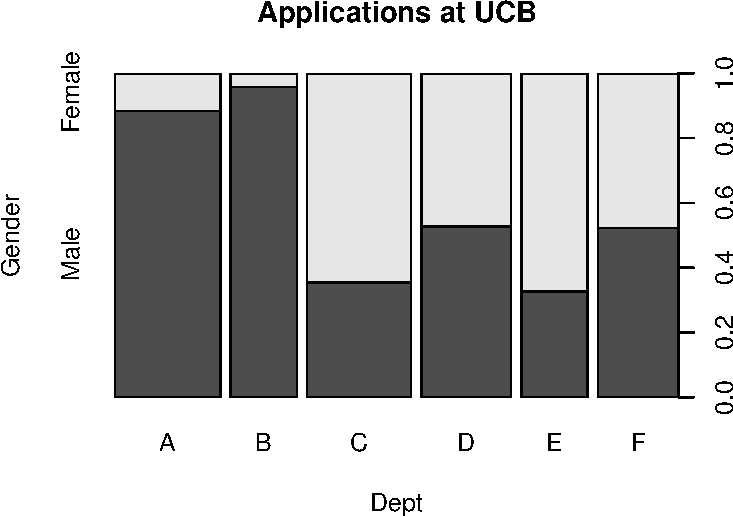
\includegraphics{index_files/figure-latex/unnamed-chunk-100-1.pdf}

\begin{Shaded}
\begin{Highlighting}[]
\KeywordTok{spineplot}\NormalTok{(}\KeywordTok{margin.table}\NormalTok{(UCBAdmissions, }\KeywordTok{c}\NormalTok{(}\DecValTok{3}\NormalTok{, }\DecValTok{1}\NormalTok{)),}
           \DataTypeTok{main =} \StringTok{"Admissions at UCB"}\NormalTok{)}
\end{Highlighting}
\end{Shaded}

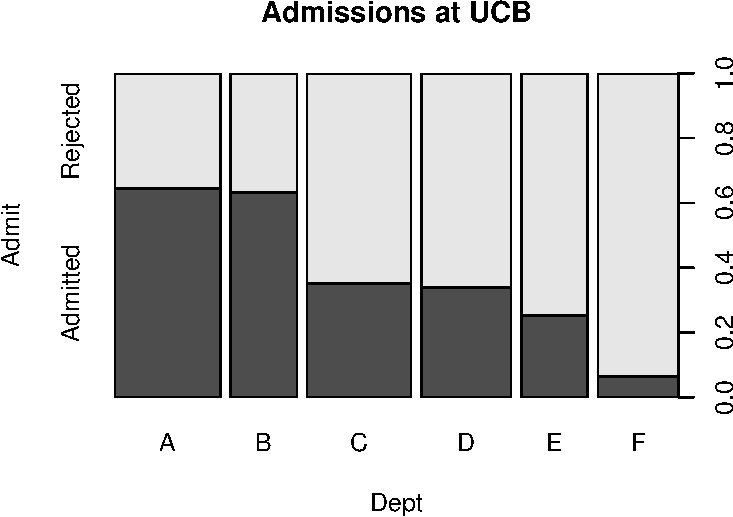
\includegraphics{index_files/figure-latex/unnamed-chunk-100-2.pdf}

This data set is frequently used for illustrating \emph{Simpson's
paradox}. At issue is whether the data show evidence of sex bias in
admission practices. There were 2691 male applicants, of whom 1198
(44.5\%) were admitted, compared with 1835 female applicants of whom 557
(30.4\%) were admitted. Men were much more successful in admissions than
women.
\href{https://en.wikipedia.org/wiki/Simpson\%27s_paradox\#UC_Berkeley_gender_bias}{Wikipedia:
Gender Bias UC Berkeley}.

\subsection{Quantitative data}\label{quantitative-data}

Quantitative data, also known as continuous data, consists of numeric
data that support arithmetic operations. This is in contrast with
qualitative data, whose values belong to pre-defined classes with no
arithmetic operation allowed. We will explain how to apply some of the R
tools for quantitative data analysis with examples.

\begin{Shaded}
\begin{Highlighting}[]
\KeywordTok{head}\NormalTok{(faithful)}
\end{Highlighting}
\end{Shaded}

\begin{verbatim}
##   eruptions waiting
## 1     3.600      79
## 2     1.800      54
## 3     3.333      74
## 4     2.283      62
## 5     4.533      85
## 6     2.883      55
\end{verbatim}

It consists of a collection of observations of the Old Faithful geyser
in the USA Yellowstone National Park.

There are two observation variables in the data set. The first one,
called \texttt{eruptions}, is the duration of the geyser eruptions. The
second one, called \texttt{waiting}, is the length of waiting period
until the next eruption. It turns out there is a correlation between the
two variables.

\begin{Shaded}
\begin{Highlighting}[]
\KeywordTok{plot}\NormalTok{(faithful)}
\end{Highlighting}
\end{Shaded}

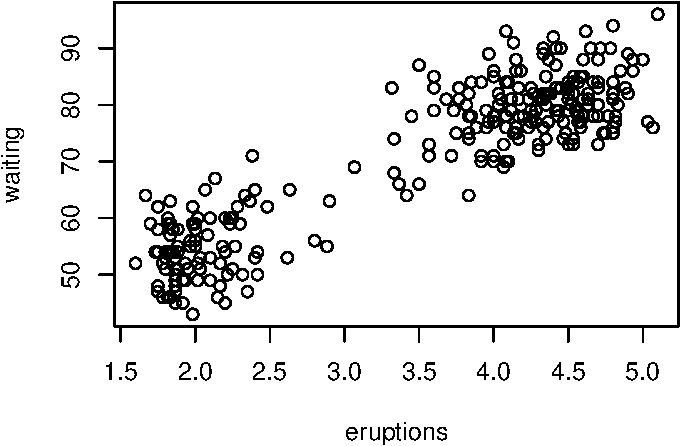
\includegraphics{index_files/figure-latex/unnamed-chunk-102-1.pdf}

\subsubsection{Frequency distribution of quantitative
data}\label{frequency-distribution-of-quantitative-data}

The frequency distribution of a data variable is a summary of the data
occurrence in a collection of non-overlapping categories.

Let us find the frequency distribution of the eruption duration in
\texttt{faithful} data set.

\begin{Shaded}
\begin{Highlighting}[]
\NormalTok{duration <-}\StringTok{ }\NormalTok{faithful$eruptions}
\KeywordTok{range}\NormalTok{(duration)}
\end{Highlighting}
\end{Shaded}

\begin{verbatim}
## [1] 1.6 5.1
\end{verbatim}

Now we create the range of non-overlapping sub-intervals by defining a
sequence of equal distance break points. If we round the endpoints of
the interval {[}1.6, 5.1{]} to the closest half-integers, we come up
with the interval {[}1.5, 5.5{]}. Hence we set the break points to be
the half-integer sequence \{ 1.5, 2.0, 2.5, \ldots{} \}.

\begin{Shaded}
\begin{Highlighting}[]
\NormalTok{breaks <-}\StringTok{ }\KeywordTok{seq}\NormalTok{(}\FloatTok{1.5}\NormalTok{,}\FloatTok{5.5}\NormalTok{,}\DataTypeTok{by=}\FloatTok{0.5}\NormalTok{)}
\NormalTok{breaks}
\end{Highlighting}
\end{Shaded}

\begin{verbatim}
## [1] 1.5 2.0 2.5 3.0 3.5 4.0 4.5 5.0 5.5
\end{verbatim}

Classify the eruption durations according to the half-unit-length
sub-intervals with cut. As the intervals are to be closed on the left,
and open on the right, we set the right argument as \texttt{FALSE}.

\begin{Shaded}
\begin{Highlighting}[]
\NormalTok{duration.cut =}\StringTok{ }\KeywordTok{cut}\NormalTok{(duration, breaks, }\DataTypeTok{right=}\OtherTok{FALSE}\NormalTok{) }
\end{Highlighting}
\end{Shaded}

Compute the frequency of eruptions in each sub-interval with the table
function.

\begin{Shaded}
\begin{Highlighting}[]
\NormalTok{duration.freq =}\StringTok{ }\KeywordTok{table}\NormalTok{(duration.cut) }
\NormalTok{duration.freq}
\end{Highlighting}
\end{Shaded}

\begin{verbatim}
## duration.cut
## [1.5,2) [2,2.5) [2.5,3) [3,3.5) [3.5,4) [4,4.5) [4.5,5) [5,5.5) 
##      51      41       5       7      30      73      61       4
\end{verbatim}

\texttt{hist} function does all the computaions to find the frequency
distribution:

\begin{Shaded}
\begin{Highlighting}[]
\NormalTok{freq <-}\StringTok{ }\KeywordTok{hist}\NormalTok{(duration)}
\NormalTok{freq}
\end{Highlighting}
\end{Shaded}

\begin{verbatim}
## $breaks
## [1] 1.5 2.0 2.5 3.0 3.5 4.0 4.5 5.0 5.5
## 
## $counts
## [1] 55 37  5  9 34 75 54  3
## 
## $density
## [1] 0.40441176 0.27205882 0.03676471 0.06617647 0.25000000 0.55147059
## [7] 0.39705882 0.02205882
## 
## $mids
## [1] 1.75 2.25 2.75 3.25 3.75 4.25 4.75 5.25
## 
## $xname
## [1] "duration"
## 
## $equidist
## [1] TRUE
## 
## attr(,"class")
## [1] "histogram"
\end{verbatim}

\begin{Shaded}
\begin{Highlighting}[]
\NormalTok{freq <-}\StringTok{ }\KeywordTok{hist}\NormalTok{(duration,}\DataTypeTok{breaks =} \NormalTok{breaks)}
\end{Highlighting}
\end{Shaded}

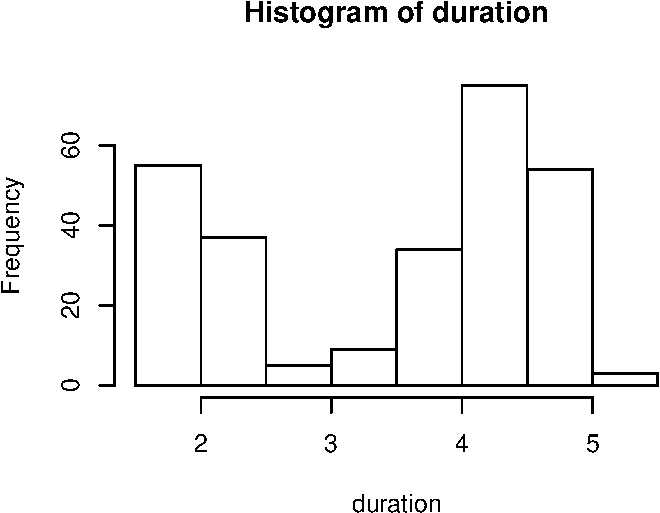
\includegraphics{index_files/figure-latex/unnamed-chunk-107-1.pdf}

\begin{Shaded}
\begin{Highlighting}[]
\KeywordTok{hist}\NormalTok{(duration,}\DecValTok{50}\NormalTok{)}
\end{Highlighting}
\end{Shaded}

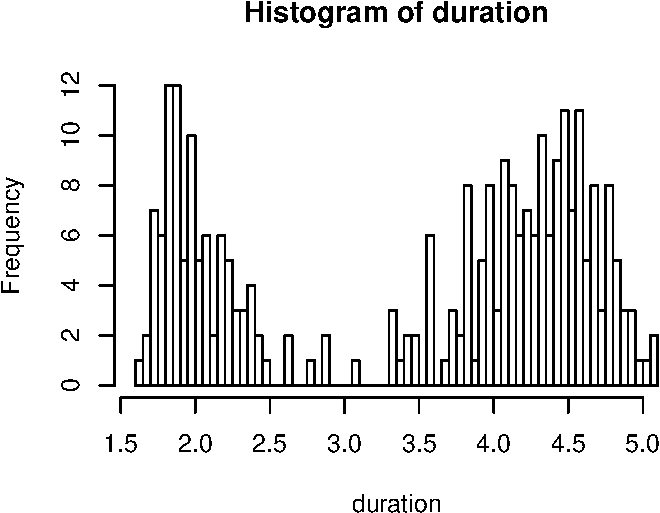
\includegraphics{index_files/figure-latex/unnamed-chunk-107-2.pdf}

\textbf{Density estimation} builds an estimate of some underlying
probability density function using an observed data sample.

\begin{Shaded}
\begin{Highlighting}[]
\KeywordTok{require}\NormalTok{(graphics)}
\NormalTok{d <-}\StringTok{ }\KeywordTok{density}\NormalTok{(faithful$eruptions)}
\NormalTok{d}
\end{Highlighting}
\end{Shaded}

\begin{verbatim}
## 
## Call:
##  density.default(x = faithful$eruptions)
## 
## Data: faithful$eruptions (272 obs.); Bandwidth 'bw' = 0.3348
## 
##        x                y            
##  Min.   :0.5957   Min.   :0.0002262  
##  1st Qu.:1.9728   1st Qu.:0.0514171  
##  Median :3.3500   Median :0.1447010  
##  Mean   :3.3500   Mean   :0.1813462  
##  3rd Qu.:4.7272   3rd Qu.:0.3086071  
##  Max.   :6.1043   Max.   :0.4842095
\end{verbatim}

\begin{Shaded}
\begin{Highlighting}[]
\KeywordTok{plot}\NormalTok{(d)}
\end{Highlighting}
\end{Shaded}

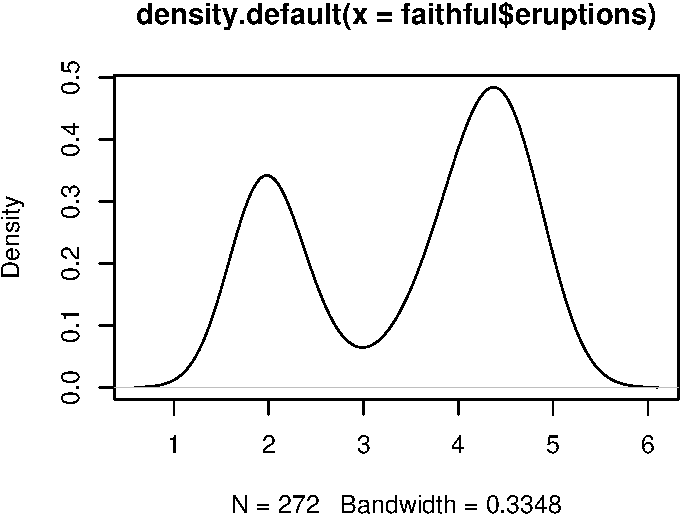
\includegraphics{index_files/figure-latex/unnamed-chunk-108-1.pdf}

Two dimension histogram:

\begin{Shaded}
\begin{Highlighting}[]
\KeywordTok{library}\NormalTok{(gplots)}
\NormalTok{h2 <-}\StringTok{ }\KeywordTok{hist2d}\NormalTok{(faithful, }\DataTypeTok{nbins=}\DecValTok{30}\NormalTok{,}\DataTypeTok{xlab=}\StringTok{"Duration in minutes"}\NormalTok{,}\DataTypeTok{ylab=}\StringTok{"Waiting"}\NormalTok{)}
\end{Highlighting}
\end{Shaded}

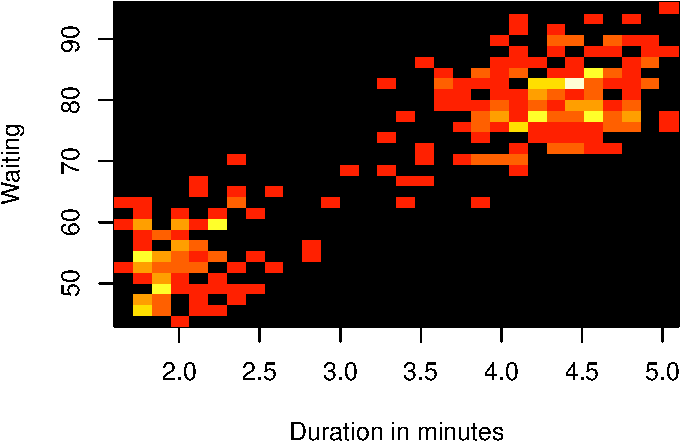
\includegraphics{index_files/figure-latex/unnamed-chunk-109-1.pdf}

\begin{Shaded}
\begin{Highlighting}[]
\NormalTok{h2}
\end{Highlighting}
\end{Shaded}

\begin{verbatim}
## 
## ----------------------------
## 2-D Histogram Object
## ----------------------------
## 
## Call: hist2d(x = faithful, nbins = 30, xlab = "Duration in minutes", 
##     ylab = "Waiting")
## 
## Number of data points:  272 
## Number of grid bins:  30 x 30 
## X range: ( 1.6 , 5.1 )
## Y range: ( 43 , 96 )
\end{verbatim}

\begin{Shaded}
\begin{Highlighting}[]
\KeywordTok{names}\NormalTok{(h2)}
\end{Highlighting}
\end{Shaded}

\begin{verbatim}
## [1] "counts"   "x.breaks" "y.breaks" "x"        "y"        "nobs"    
## [7] "call"
\end{verbatim}

Relative frequencies

\begin{Shaded}
\begin{Highlighting}[]
\NormalTok{duration.relfreq <-}\StringTok{ }\NormalTok{duration.freq /}\StringTok{ }\KeywordTok{nrow}\NormalTok{(faithful) }
\NormalTok{tab <-}\StringTok{ }\KeywordTok{cbind}\NormalTok{(duration.freq, duration.relfreq) }
\KeywordTok{apply}\NormalTok{(tab,}\DecValTok{2}\NormalTok{,sum)}
\end{Highlighting}
\end{Shaded}

\begin{verbatim}
##    duration.freq duration.relfreq 
##              272                1
\end{verbatim}

Cumulative frequency distribution

\begin{Shaded}
\begin{Highlighting}[]
\KeywordTok{cumsum}\NormalTok{(duration.freq)}
\end{Highlighting}
\end{Shaded}

\begin{verbatim}
## [1.5,2) [2,2.5) [2.5,3) [3,3.5) [3.5,4) [4,4.5) [4.5,5) [5,5.5) 
##      51      92      97     104     134     207     268     272
\end{verbatim}

\begin{Shaded}
\begin{Highlighting}[]
\KeywordTok{cumsum}\NormalTok{(duration.relfreq)}
\end{Highlighting}
\end{Shaded}

\begin{verbatim}
##   [1.5,2)   [2,2.5)   [2.5,3)   [3,3.5)   [3.5,4)   [4,4.5)   [4.5,5) 
## 0.1875000 0.3382353 0.3566176 0.3823529 0.4926471 0.7610294 0.9852941 
##   [5,5.5) 
## 1.0000000
\end{verbatim}

We can plot the cumulative relative frequency graph of a quantitative
variable, which is a curve graphically showing the cumulative relative
frequency distribution. The e.c.d.f. (empirical cumulative distribution
function) \(F_n\) is a step function with jumps \(i/n\) at observation
values, where \(i\) is the number of tied observations at that value.
Missing values are ignored.

For observations \(x = (x_1,x_2, ... x_n)\), \(F_n\) is the fraction of
observations less or equal to \(t\), i.e.,

\[
F_n(t) = \#{x_i <= t}/n = 1/n \sum_{i=1}^n I(x_i \leq t).
\] where \(I\) is an indication function.

\begin{Shaded}
\begin{Highlighting}[]
\KeywordTok{plot}\NormalTok{(}\KeywordTok{ecdf}\NormalTok{(duration))}
\end{Highlighting}
\end{Shaded}

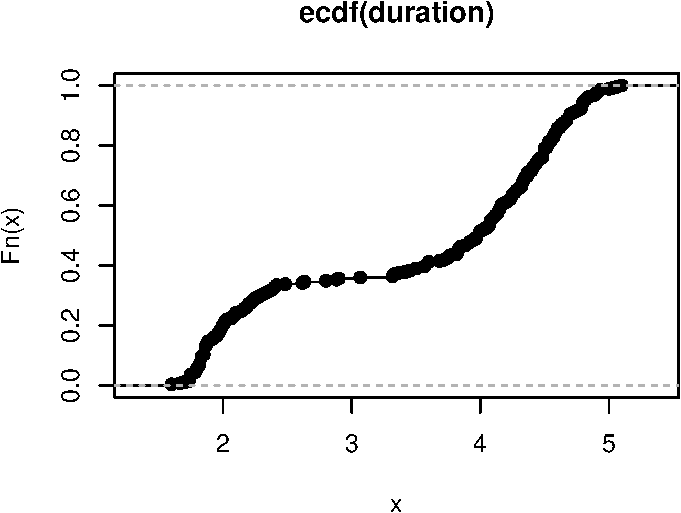
\includegraphics{index_files/figure-latex/unnamed-chunk-112-1.pdf}

\textbf{Bivariante Density estimation:}

\begin{Shaded}
\begin{Highlighting}[]
\KeywordTok{data}\NormalTok{(}\StringTok{"faithful"}\NormalTok{)}
\KeywordTok{attach}\NormalTok{(faithful)}
\NormalTok{Dens2d<-}\KeywordTok{kde2d}\NormalTok{(eruptions,waiting)}
\KeywordTok{image}\NormalTok{(Dens2d,}\DataTypeTok{xlab=}\StringTok{"eruptions"}\NormalTok{,}\DataTypeTok{ylab=}\StringTok{"waiting"}\NormalTok{)}
\KeywordTok{contour}\NormalTok{(Dens2d,}\DataTypeTok{add=}\OtherTok{TRUE}\NormalTok{,}\DataTypeTok{col=}\StringTok{"black"}\NormalTok{,}\DataTypeTok{lwd=}\DecValTok{2}\NormalTok{,}\DataTypeTok{nlevels=}\DecValTok{5}\NormalTok{)}
\end{Highlighting}
\end{Shaded}

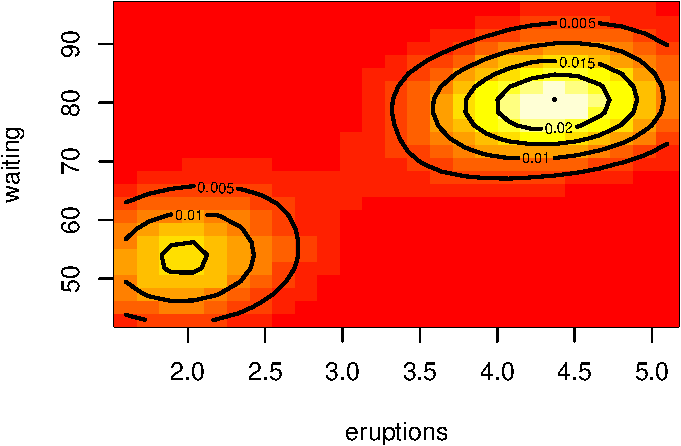
\includegraphics{index_files/figure-latex/unnamed-chunk-113-1.pdf}

\begin{Shaded}
\begin{Highlighting}[]
\KeywordTok{detach}\NormalTok{(}\StringTok{"faithful"}\NormalTok{)}
\end{Highlighting}
\end{Shaded}

\textbf{Perspective plot:}

\begin{Shaded}
\begin{Highlighting}[]
\KeywordTok{persp}\NormalTok{(Dens2d,}\DataTypeTok{phi=}\DecValTok{30}\NormalTok{,}\DataTypeTok{theta=}\DecValTok{20}\NormalTok{,}\DataTypeTok{d=}\DecValTok{5}\NormalTok{,}\DataTypeTok{xlab=}\StringTok{"eruptions"}\NormalTok{,}\DataTypeTok{ylab=}\StringTok{"waiting"}\NormalTok{,}\DataTypeTok{zlab=}\StringTok{""}\NormalTok{,}\DataTypeTok{shade=}\NormalTok{.}\DecValTok{2}\NormalTok{,}\DataTypeTok{col=}\StringTok{"lightblue"}\NormalTok{,}\DataTypeTok{expand=}\NormalTok{.}\DecValTok{85}\NormalTok{,}\DataTypeTok{ticktype =} \StringTok{"detailed"}\NormalTok{)}
\end{Highlighting}
\end{Shaded}

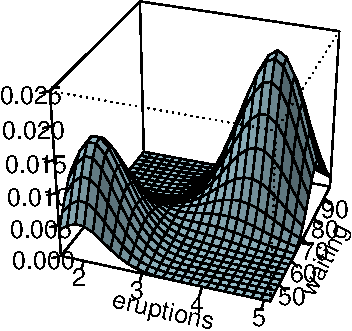
\includegraphics{index_files/figure-latex/unnamed-chunk-114-1.pdf}

\section{\texorpdfstring{Introduction to basic programming in
\texttt{R}}{Introduction to basic programming in R}}\label{introduction-to-basic-programming-in-r}

\subsection{Control Structures}\label{control-structures}

\subsubsection{Conditional Executions}\label{conditional-executions}

\paragraph{Comparison Operators}\label{comparison-operators}

\begin{itemize}
\tightlist
\item
  equal: \texttt{==}
\end{itemize}

\begin{Shaded}
\begin{Highlighting}[]
  \StringTok{"hola"} \NormalTok{==}\StringTok{ "hola"}
\end{Highlighting}
\end{Shaded}

\begin{verbatim}
## [1] TRUE
\end{verbatim}

\begin{Shaded}
\begin{Highlighting}[]
  \StringTok{"hola"} \NormalTok{==}\StringTok{ "Hola"}
\end{Highlighting}
\end{Shaded}

\begin{verbatim}
## [1] FALSE
\end{verbatim}

\begin{Shaded}
\begin{Highlighting}[]
   \DecValTok{1} \NormalTok{==}\StringTok{ }\DecValTok{2-1}
\end{Highlighting}
\end{Shaded}

\begin{verbatim}
## [1] TRUE
\end{verbatim}

\begin{itemize}
\tightlist
\item
  not equal: \texttt{!=}
\end{itemize}

\begin{Shaded}
\begin{Highlighting}[]
    \NormalTok{a <-}\StringTok{ }\KeywordTok{c}\NormalTok{(}\DecValTok{1}\NormalTok{,}\DecValTok{2}\NormalTok{,}\DecValTok{4}\NormalTok{,}\DecValTok{5}\NormalTok{)}
    \NormalTok{b <-}\StringTok{ }\KeywordTok{c}\NormalTok{(}\DecValTok{1}\NormalTok{,}\DecValTok{2}\NormalTok{,}\DecValTok{3}\NormalTok{,}\DecValTok{5}\NormalTok{) }
    \NormalTok{a ==}\StringTok{ }\NormalTok{b}
\end{Highlighting}
\end{Shaded}

\begin{verbatim}
## [1]  TRUE  TRUE FALSE  TRUE
\end{verbatim}

\begin{Shaded}
\begin{Highlighting}[]
    \NormalTok{a !=}\StringTok{ }\NormalTok{b}
\end{Highlighting}
\end{Shaded}

\begin{verbatim}
## [1] FALSE FALSE  TRUE FALSE
\end{verbatim}

\begin{itemize}
\tightlist
\item
  greater/less than: \texttt{\textgreater{}} \texttt{\textless{}}
\end{itemize}

\begin{Shaded}
\begin{Highlighting}[]
\KeywordTok{set.seed}\NormalTok{(}\DecValTok{1}\NormalTok{)}
\NormalTok{a <-}\StringTok{ }\KeywordTok{rnorm}\NormalTok{(}\DecValTok{10}\NormalTok{,}\DecValTok{3}\NormalTok{,}\DecValTok{1}\NormalTok{)}
\NormalTok{b <-}\StringTok{ }\KeywordTok{rnorm}\NormalTok{(}\DecValTok{10}\NormalTok{,}\DecValTok{4}\NormalTok{,}\DecValTok{2}\NormalTok{)}
\NormalTok{a<b}
\end{Highlighting}
\end{Shaded}

\begin{verbatim}
##  [1]  TRUE  TRUE  TRUE FALSE  TRUE  TRUE  TRUE  TRUE  TRUE  TRUE
\end{verbatim}

\begin{itemize}
\tightlist
\item
  greater/less than or equal: \texttt{\textgreater{}=}
  \texttt{\textless{}=}
\end{itemize}

\begin{Shaded}
\begin{Highlighting}[]
\KeywordTok{set.seed}\NormalTok{(}\DecValTok{1}\NormalTok{)}
\NormalTok{a <-}\StringTok{ }\KeywordTok{rpois}\NormalTok{(}\DecValTok{10}\NormalTok{,}\DecValTok{1}\NormalTok{)}
\NormalTok{b <-}\StringTok{ }\KeywordTok{rbinom}\NormalTok{(}\DecValTok{10}\NormalTok{,}\DecValTok{2}\NormalTok{,.}\DecValTok{56}\NormalTok{)}
\NormalTok{a >=}\StringTok{ }\NormalTok{b}
\end{Highlighting}
\end{Shaded}

\begin{verbatim}
##  [1] FALSE FALSE  TRUE  TRUE FALSE  TRUE  TRUE  TRUE  TRUE FALSE
\end{verbatim}

\begin{itemize}
\tightlist
\item
  \texttt{which}
\end{itemize}

\begin{Shaded}
\begin{Highlighting}[]
\KeywordTok{set.seed}\NormalTok{(}\DecValTok{1}\NormalTok{)}
\KeywordTok{which}\NormalTok{(a>b)}
\end{Highlighting}
\end{Shaded}

\begin{verbatim}
## [1] 4 6 7 8
\end{verbatim}

\begin{Shaded}
\begin{Highlighting}[]
\NormalTok{LETTERS}
\end{Highlighting}
\end{Shaded}

\begin{verbatim}
##  [1] "A" "B" "C" "D" "E" "F" "G" "H" "I" "J" "K" "L" "M" "N" "O" "P" "Q"
## [18] "R" "S" "T" "U" "V" "W" "X" "Y" "Z"
\end{verbatim}

\begin{Shaded}
\begin{Highlighting}[]
\KeywordTok{which}\NormalTok{(LETTERS==}\StringTok{"R"}\NormalTok{)}
\end{Highlighting}
\end{Shaded}

\begin{verbatim}
## [1] 18
\end{verbatim}

\begin{itemize}
\tightlist
\item
  \texttt{which.min} or \texttt{which.max}
\end{itemize}

\begin{Shaded}
\begin{Highlighting}[]
\KeywordTok{set.seed}\NormalTok{(}\DecValTok{1}\NormalTok{)}
\NormalTok{a <-}\StringTok{ }\KeywordTok{rnorm}\NormalTok{(}\DecValTok{10}\NormalTok{,}\DecValTok{2}\NormalTok{,}\DecValTok{1}\NormalTok{)}
\NormalTok{a}
\end{Highlighting}
\end{Shaded}

\begin{verbatim}
##  [1] 1.373546 2.183643 1.164371 3.595281 2.329508 1.179532 2.487429
##  [8] 2.738325 2.575781 1.694612
\end{verbatim}

\begin{Shaded}
\begin{Highlighting}[]
\KeywordTok{which.min}\NormalTok{(a)}
\end{Highlighting}
\end{Shaded}

\begin{verbatim}
## [1] 3
\end{verbatim}

\begin{Shaded}
\begin{Highlighting}[]
\KeywordTok{which.max}\NormalTok{(a)}
\end{Highlighting}
\end{Shaded}

\begin{verbatim}
## [1] 4
\end{verbatim}

\begin{itemize}
\tightlist
\item
  \texttt{is.na}
\end{itemize}

\begin{Shaded}
\begin{Highlighting}[]
 \NormalTok{a[}\DecValTok{2}\NormalTok{] <-}\StringTok{ }\OtherTok{NA}
\KeywordTok{is.na}\NormalTok{(a)}
\end{Highlighting}
\end{Shaded}

\begin{verbatim}
##  [1] FALSE  TRUE FALSE FALSE FALSE FALSE FALSE FALSE FALSE FALSE
\end{verbatim}

\begin{Shaded}
\begin{Highlighting}[]
\KeywordTok{which}\NormalTok{(}\KeywordTok{is.na}\NormalTok{(a))}
\end{Highlighting}
\end{Shaded}

\begin{verbatim}
## [1] 2
\end{verbatim}

\subsubsection{Logical Operators}\label{logical-operators}

\begin{itemize}
\tightlist
\item
  and: \texttt{\&}
\end{itemize}

\begin{Shaded}
\begin{Highlighting}[]
\NormalTok{z =}\StringTok{ }\DecValTok{1}\NormalTok{:}\DecValTok{6}
\KeywordTok{which}\NormalTok{(}\DecValTok{2} \NormalTok{<}\StringTok{ }\NormalTok{z &}\StringTok{ }\NormalTok{z >}\StringTok{ }\DecValTok{3}\NormalTok{)}
\end{Highlighting}
\end{Shaded}

\begin{verbatim}
## [1] 4 5 6
\end{verbatim}

\begin{itemize}
\tightlist
\item
  or: \texttt{\textbar{}}
\end{itemize}

\begin{Shaded}
\begin{Highlighting}[]
\NormalTok{z =}\StringTok{ }\DecValTok{1}\NormalTok{:}\DecValTok{6}
\NormalTok{(z >}\StringTok{ }\DecValTok{2}\NormalTok{) &}\StringTok{ }\NormalTok{(z <}\StringTok{ }\DecValTok{5}\NormalTok{)}
\end{Highlighting}
\end{Shaded}

\begin{verbatim}
## [1] FALSE FALSE  TRUE  TRUE FALSE FALSE
\end{verbatim}

\begin{Shaded}
\begin{Highlighting}[]
\KeywordTok{which}\NormalTok{((z >}\StringTok{ }\DecValTok{2}\NormalTok{) &}\StringTok{ }\NormalTok{(z <}\StringTok{ }\DecValTok{5}\NormalTok{))}
\end{Highlighting}
\end{Shaded}

\begin{verbatim}
## [1] 3 4
\end{verbatim}

\begin{itemize}
\tightlist
\item
  not: \texttt{!}
\end{itemize}

\begin{Shaded}
\begin{Highlighting}[]
\NormalTok{x <-}\StringTok{ }\KeywordTok{c}\NormalTok{(}\OtherTok{TRUE}\NormalTok{,}\OtherTok{FALSE}\NormalTok{,}\DecValTok{0}\NormalTok{,}\DecValTok{6}\NormalTok{)}
\NormalTok{y <-}\StringTok{ }\KeywordTok{c}\NormalTok{(}\OtherTok{FALSE}\NormalTok{,}\OtherTok{TRUE}\NormalTok{,}\OtherTok{FALSE}\NormalTok{,}\OtherTok{TRUE}\NormalTok{)}

\NormalTok{!x}
\end{Highlighting}
\end{Shaded}

\begin{verbatim}
## [1] FALSE  TRUE  TRUE FALSE
\end{verbatim}

Operators \texttt{\&} and \texttt{\textbar{}} perform element-wise
operation producing result having length of the longer operand. But
\texttt{\&\&} and \texttt{\textbar{}\textbar{}} examines only the first
element of the operands resulting into a single length logical vector.
Zero is considered \texttt{FALSE} and non-zero numbers are taken as
\texttt{TRUE}. \textbf{Example:}

\begin{itemize}
\tightlist
\item
  \texttt{\&\&} vs \texttt{\&}
\end{itemize}

\begin{Shaded}
\begin{Highlighting}[]
\NormalTok{x&y}
\end{Highlighting}
\end{Shaded}

\begin{verbatim}
## [1] FALSE FALSE FALSE  TRUE
\end{verbatim}

\begin{Shaded}
\begin{Highlighting}[]
\NormalTok{x&&y}
\end{Highlighting}
\end{Shaded}

\begin{verbatim}
## [1] FALSE
\end{verbatim}

\begin{itemize}
\tightlist
\item
  \texttt{\textbar{}\textbar{}} vs \texttt{\textbar{}}
\end{itemize}

\begin{Shaded}
\begin{Highlighting}[]
\NormalTok{x||y}
\end{Highlighting}
\end{Shaded}

\begin{verbatim}
## [1] TRUE
\end{verbatim}

\begin{Shaded}
\begin{Highlighting}[]
\NormalTok{x|y}
\end{Highlighting}
\end{Shaded}

\begin{verbatim}
## [1]  TRUE  TRUE FALSE  TRUE
\end{verbatim}

\subsection{\texorpdfstring{\texttt{if}
statements}{if statements}}\label{if-statements}

\texttt{if(cond1=true)\ \{\ cmd1\ \}\ else\ \{\ cmd2\ \}}

\begin{Shaded}
\begin{Highlighting}[]
\NormalTok{if(}\DecValTok{1}\NormalTok{==}\DecValTok{0}\NormalTok{) \{}
    \KeywordTok{print}\NormalTok{(}\DecValTok{1}\NormalTok{)}
\NormalTok{\} else \{}
    \KeywordTok{print}\NormalTok{(}\DecValTok{2}\NormalTok{)}
\NormalTok{\}}
\end{Highlighting}
\end{Shaded}

\begin{verbatim}
## [1] 2
\end{verbatim}

\subsection{\texorpdfstring{\texttt{ifelse}
statement}{ifelse statement}}\label{ifelse-statement}

\texttt{ifelse(test,\ true\_value,\ false\_value)}

\begin{Shaded}
\begin{Highlighting}[]
\NormalTok{x <-}\StringTok{ }\DecValTok{1}\NormalTok{:}\DecValTok{10} \CommentTok{# Creates sample data}
\KeywordTok{ifelse}\NormalTok{(x<}\DecValTok{5} \NormalTok{|}\StringTok{ }\NormalTok{x>}\DecValTok{8}\NormalTok{, x, }\DecValTok{0}\NormalTok{)}
\end{Highlighting}
\end{Shaded}

\begin{verbatim}
##  [1]  1  2  3  4  0  0  0  0  9 10
\end{verbatim}

\subsection{\texorpdfstring{\texttt{while}
statement}{while statement}}\label{while-statement}

\subsection{Loops}\label{loops}

The most commonly used loop structures in \texttt{R} are \texttt{for},
\texttt{while} and \texttt{apply} loops. Less common are \texttt{repeat}
loops. The \texttt{break} function is used to break out of loops, and
next halts the processing of the current iteration and advances the
looping index.

\subsubsection{\texorpdfstring{\texttt{for}}{for}}\label{for}

For loops are controlled by a looping vector. In every iteration of the
loop one value in the looping vector is assigned to a variable that can
be used in the statements of the body of the loop. Usually, the number
of loop iterations is defined by the number of values stored in the
looping vector and they are processed in the same order as they are
stored in the looping vector.

Syntax

\begin{verbatim}
for(variable in sequence) {
    statements
}
\end{verbatim}

\begin{Shaded}
\begin{Highlighting}[]
\NormalTok{for (j in }\DecValTok{1}\NormalTok{:}\DecValTok{5}\NormalTok{)}
\NormalTok{\{}
  \KeywordTok{print}\NormalTok{(j^}\DecValTok{2}\NormalTok{)}
\NormalTok{\}}
\end{Highlighting}
\end{Shaded}

\begin{verbatim}
## [1] 1
## [1] 4
## [1] 9
## [1] 16
## [1] 25
\end{verbatim}

Repeat the loop saving the resuls in a vector \texttt{x}.

\begin{Shaded}
\begin{Highlighting}[]
\NormalTok{n =}\StringTok{ }\DecValTok{5}
\NormalTok{x =}\StringTok{ }\OtherTok{NULL}  \CommentTok{# creates a NULL object}
\NormalTok{for (j in }\DecValTok{1}\NormalTok{:n)}
\NormalTok{\{}
  \NormalTok{x[j] =}\StringTok{ }\NormalTok{j^}\DecValTok{2}
\NormalTok{\}}
\NormalTok{x}
\end{Highlighting}
\end{Shaded}

\begin{verbatim}
## [1]  1  4  9 16 25
\end{verbatim}

Let's use a for loop to estimate the average of squaring the result of a
roll of a dice.

\begin{Shaded}
\begin{Highlighting}[]
\NormalTok{nsides =}\StringTok{ }\DecValTok{6}
\NormalTok{ntrials =}\StringTok{ }\DecValTok{1000}
\NormalTok{trials =}\StringTok{ }\OtherTok{NULL}
\NormalTok{for (j in }\DecValTok{1}\NormalTok{:ntrials)}
\NormalTok{\{}
  \NormalTok{trials[j] =}\StringTok{ }\KeywordTok{sample}\NormalTok{(}\DecValTok{1}\NormalTok{:nsides,}\DecValTok{1}\NormalTok{)  }\CommentTok{# We get one sample at a time}
\NormalTok{\}}
\KeywordTok{mean}\NormalTok{(trials^}\DecValTok{2}\NormalTok{)}
\end{Highlighting}
\end{Shaded}

\begin{verbatim}
## [1] 15.122
\end{verbatim}

\textbf{Example:} stop on condition and print error message

\begin{Shaded}
\begin{Highlighting}[]
\NormalTok{x <-}\StringTok{ }\DecValTok{1}\NormalTok{:}\DecValTok{10}
\NormalTok{z <-}\StringTok{ }\OtherTok{NULL}
\NormalTok{for(i in }\KeywordTok{seq}\NormalTok{(}\DataTypeTok{along=}\NormalTok{x)) \{}
    \NormalTok{if (x[i]<}\DecValTok{5}\NormalTok{) \{}
        \NormalTok{z <-}\StringTok{ }\KeywordTok{c}\NormalTok{(z,x[i]-}\DecValTok{1}\NormalTok{) }
    \NormalTok{\} else \{}
        \KeywordTok{stop}\NormalTok{(}\StringTok{"values need to be <5"}\NormalTok{)}
    \NormalTok{\}}
\NormalTok{\}}
\NormalTok{## Error: values need to be <5}
\NormalTok{z}
\NormalTok{## [1] 0 1 2 3}
\end{Highlighting}
\end{Shaded}

\subsection{\texorpdfstring{\texttt{while}}{while}}\label{while}

Similar to \texttt{for} loop, but the iterations are controlled by a
conditional statement.

\begin{Shaded}
\begin{Highlighting}[]
\NormalTok{z <-}\StringTok{ }\DecValTok{0}
\NormalTok{while(z <}\StringTok{ }\DecValTok{5}\NormalTok{) \{}
    \NormalTok{z <-}\StringTok{ }\NormalTok{z +}\StringTok{ }\DecValTok{2}
    \KeywordTok{print}\NormalTok{(z) }
\NormalTok{\}}
\end{Highlighting}
\end{Shaded}

\begin{verbatim}
## [1] 2
## [1] 4
## [1] 6
\end{verbatim}

\subsection{\texorpdfstring{\texttt{apply} loop
family}{apply loop family}}\label{apply-loop-family}

For Two-Dimensional Data Sets: apply

\textbf{Syntax:}

\begin{verbatim}
apply(X, MARGIN, FUN, ARGs)
\end{verbatim}

\texttt{X}: \texttt{array}, \texttt{matrix} or \texttt{data.frame};
\texttt{MARGIN}: 1 for rows, 2 for columns, \texttt{c(1,2)} for both;
\texttt{FUN}: one or more functions; \texttt{ARGs}: possible arguments
for function.

\begin{Shaded}
\begin{Highlighting}[]
\NormalTok{## Example for applying predefined mean function}
\KeywordTok{apply}\NormalTok{(mtcars[,}\DecValTok{1}\NormalTok{:}\DecValTok{3}\NormalTok{], }\DecValTok{1}\NormalTok{, mean)}

\NormalTok{## With custom function}
\NormalTok{x <-}\StringTok{ }\DecValTok{1}\NormalTok{:}\DecValTok{10}
\NormalTok{test <-}\StringTok{ }\NormalTok{function(x) \{ }\CommentTok{# Defines some custom function}
    \NormalTok{if(x <}\StringTok{ }\DecValTok{5}\NormalTok{) \{}
        \NormalTok{x}\DecValTok{-1}
    \NormalTok{\} else \{}
        \NormalTok{x /}\StringTok{ }\NormalTok{x}
    \NormalTok{\}}
\NormalTok{\} }

\KeywordTok{apply}\NormalTok{(}\KeywordTok{as.matrix}\NormalTok{(x), }\DecValTok{1}\NormalTok{, test) }

\NormalTok{## Same as above but with a single line of code}
\KeywordTok{apply}\NormalTok{(}\KeywordTok{as.matrix}\NormalTok{(x), }\DecValTok{1}\NormalTok{, function(x) \{ if (x<}\DecValTok{5}\NormalTok{) \{ x}\DecValTok{-1} \NormalTok{\} else \{ x/x \} \})}
\end{Highlighting}
\end{Shaded}

\textbf{For Ragged Arrays: \texttt{tapply}}

Apply a function to each cell of a ragged array, that is to each
(non-empty) group of values given by a unique combination of the levels
of certain factors.

\begin{Shaded}
\begin{Highlighting}[]
\NormalTok{## Computes mean values of vector agregates defined by factor}
\KeywordTok{tapply}\NormalTok{(}\KeywordTok{as.vector}\NormalTok{(mtcars$mpg), }\KeywordTok{factor}\NormalTok{(mtcars$cyl), mean)}
\end{Highlighting}
\end{Shaded}

\begin{verbatim}
##        4        6        8 
## 26.66364 19.74286 15.10000
\end{verbatim}

\begin{Shaded}
\begin{Highlighting}[]
\NormalTok{## The aggregate function provides related utilities}
\KeywordTok{aggregate}\NormalTok{(mtcars[,}\KeywordTok{c}\NormalTok{(}\DecValTok{1}\NormalTok{,}\DecValTok{3}\NormalTok{,}\DecValTok{4}\NormalTok{)], }\KeywordTok{list}\NormalTok{(mtcars$cyl), mean)}
\end{Highlighting}
\end{Shaded}

\begin{verbatim}
##   Group.1      mpg     disp        hp
## 1       4 26.66364 105.1364  82.63636
## 2       6 19.74286 183.3143 122.28571
## 3       8 15.10000 353.1000 209.21429
\end{verbatim}

\textbf{For Vectors and Lists: \texttt{lapply} and \texttt{sapply}}

Both apply a function to vector or list objects. The function
\texttt{lapply} returns a list, while \texttt{sapply} attempts to return
the simplest data object, such as \texttt{vector} or \texttt{matrix}
instead of \texttt{list}.

\emph{Syntax}

\begin{verbatim}
lapply(X,FUN)
sapply(X,FUN)
\end{verbatim}

\begin{Shaded}
\begin{Highlighting}[]
\NormalTok{## Creates a sample list}
\NormalTok{mylist <-}\StringTok{ }\KeywordTok{as.list}\NormalTok{(mtcars[,}\KeywordTok{c}\NormalTok{(}\DecValTok{1}\NormalTok{,}\DecValTok{4}\NormalTok{,}\DecValTok{6}\NormalTok{)])}
\NormalTok{mylist}
\end{Highlighting}
\end{Shaded}

\begin{verbatim}
## $mpg
##  [1] 21.0 21.0 22.8 21.4 18.7 18.1 14.3 24.4 22.8 19.2 17.8 16.4 17.3 15.2
## [15] 10.4 10.4 14.7 32.4 30.4 33.9 21.5 15.5 15.2 13.3 19.2 27.3 26.0 30.4
## [29] 15.8 19.7 15.0 21.4
## 
## $hp
##  [1] 110 110  93 110 175 105 245  62  95 123 123 180 180 180 205 215 230
## [18]  66  52  65  97 150 150 245 175  66  91 113 264 175 335 109
## 
## $wt
##  [1] 2.620 2.875 2.320 3.215 3.440 3.460 3.570 3.190 3.150 3.440 3.440
## [12] 4.070 3.730 3.780 5.250 5.424 5.345 2.200 1.615 1.835 2.465 3.520
## [23] 3.435 3.840 3.845 1.935 2.140 1.513 3.170 2.770 3.570 2.780
\end{verbatim}

Compute sum of each list component and return result as list

\begin{Shaded}
\begin{Highlighting}[]
\KeywordTok{lapply}\NormalTok{(mylist, sum)}
\end{Highlighting}
\end{Shaded}

\begin{verbatim}
## $mpg
## [1] 642.9
## 
## $hp
## [1] 4694
## 
## $wt
## [1] 102.952
\end{verbatim}

Compute sum of each list component and return result as vector

\begin{Shaded}
\begin{Highlighting}[]
\KeywordTok{sapply}\NormalTok{(mylist, sum)}
\end{Highlighting}
\end{Shaded}

\begin{verbatim}
##      mpg       hp       wt 
##  642.900 4694.000  102.952
\end{verbatim}

\subsection{Other Loops}\label{other-loops}

\textbf{Repeat Loop}

\emph{Syntax}

\texttt{repeat} statements

Loop is repeated until a break is specified. This means there needs to
be a second statement to test whether or not to break from the loop.

\emph{Example:}

\begin{verbatim}
z <- 0
repeat {
    z <- z + 1
    print(z)
    if(z > 100) break()
}
\end{verbatim}

\subsection{Improving Speed Performance of
Loops}\label{improving-speed-performance-of-loops}

Looping over very large data sets can become slow in \texttt{R}.
However, this limitation can be overcome by eliminating certain
operations in loops or avoiding loops over the data intensive dimension
in an object altogether. The latter can be achieved by performing mainly
vector-to-vector or matrix-to-matrix computations which run often over
100 times faster than the corresponding \texttt{for()} or
\texttt{apply()} loops in \texttt{R}. For this purpose, one can make use
of the existing speed-optimized R functions (e.g.: \texttt{rowSums},
\texttt{rowMeans}, \texttt{table}, \texttt{tabulate}) or one can design
custom functions that avoid expensive \texttt{R} loops by using vector-
or matrix-based approaches. Alternatively, one can write programs that
will perform all time consuming computations on the C-level.

\begin{enumerate}
\def\labelenumi{\arabic{enumi}.}
\tightlist
\item
  Speed comparison of \texttt{for} loops with an append versus and
  inject step
\end{enumerate}

\begin{Shaded}
\begin{Highlighting}[]
\NormalTok{N <-}\StringTok{ }\FloatTok{1e6}
\NormalTok{myMA <-}\StringTok{ }\KeywordTok{matrix}\NormalTok{(}\KeywordTok{rnorm}\NormalTok{(N), N, }\DecValTok{10}\NormalTok{, }\DataTypeTok{dimnames=}\KeywordTok{list}\NormalTok{(}\DecValTok{1}\NormalTok{:N, }\KeywordTok{paste}\NormalTok{(}\StringTok{"C"}\NormalTok{, }\DecValTok{1}\NormalTok{:}\DecValTok{10}\NormalTok{, }\DataTypeTok{sep=}\StringTok{""}\NormalTok{)))}
\NormalTok{results <-}\StringTok{ }\OtherTok{NULL}
\KeywordTok{system.time}\NormalTok{(for(i in }\KeywordTok{seq}\NormalTok{(}\DataTypeTok{along=}\NormalTok{myMA[,}\DecValTok{1}\NormalTok{])) }
            \NormalTok{results <-}\StringTok{ }\KeywordTok{c}\NormalTok{(results, }\KeywordTok{mean}\NormalTok{(myMA[i,])))}

\NormalTok{results <-}\StringTok{ }\KeywordTok{numeric}\NormalTok{(}\KeywordTok{length}\NormalTok{(myMA[,}\DecValTok{1}\NormalTok{]))}
\KeywordTok{system.time}\NormalTok{(for(i in }\KeywordTok{seq}\NormalTok{(}\DataTypeTok{along=}\NormalTok{myMA[,}\DecValTok{1}\NormalTok{])) }
            \NormalTok{results[i] <-}\StringTok{ }\KeywordTok{mean}\NormalTok{(myMA[i,]))}
\end{Highlighting}
\end{Shaded}

The inject approach is 20-50 times faster than the append version.

\begin{enumerate}
\def\labelenumi{\arabic{enumi}.}
\setcounter{enumi}{1}
\tightlist
\item
  Speed comparison of \texttt{apply} loop versus \texttt{rowMeans} for
  computing the mean for each row in a large matrix:
\end{enumerate}

\begin{Shaded}
\begin{Highlighting}[]
\KeywordTok{system.time}\NormalTok{(myMAmean <-}\StringTok{ }\KeywordTok{apply}\NormalTok{(myMA, }\DecValTok{1}\NormalTok{, mean))}
\KeywordTok{system.time}\NormalTok{(myMAmean <-}\StringTok{ }\KeywordTok{rowMeans}\NormalTok{(myMA))}
\end{Highlighting}
\end{Shaded}

The \texttt{rowMeans} approach is over 200 times faster than the
\texttt{apply} loop.

\section{Probability distributions}\label{probability-distributions}

\subsection{\texorpdfstring{Binomial distribution
\(Bin(n,p)\)}{Binomial distribution Bin(n,p)}}\label{binomial-distribution-binnp}

The binomial distribution is a discrete probability distribution. It
describes the outcome of \(n\) independent trials in an experiment. Each
trial is assumed to have only two outcomes, either success or failure.
If the probability of a successful trial is \(p\), then the probability
of having \(k\) successful outcomes in an experiment of \(n\)
independent trials is given by the \textbf{probability mass function}:.

\[
f(k,n,p) = \mbox{Pr}(X=k)=\binom{n}{k} p^k (1-p)^{n-k}, \quad k=0,1,2,...,n
\]

The \textbf{cumulative distribution function} can be expressed as:

\[
F(k;n,p) = \mbox{Pr}(X\leq k) = \sum_{i=0}^{k}\binom{n}{i} p^i (1-p)^{n-i}
\] 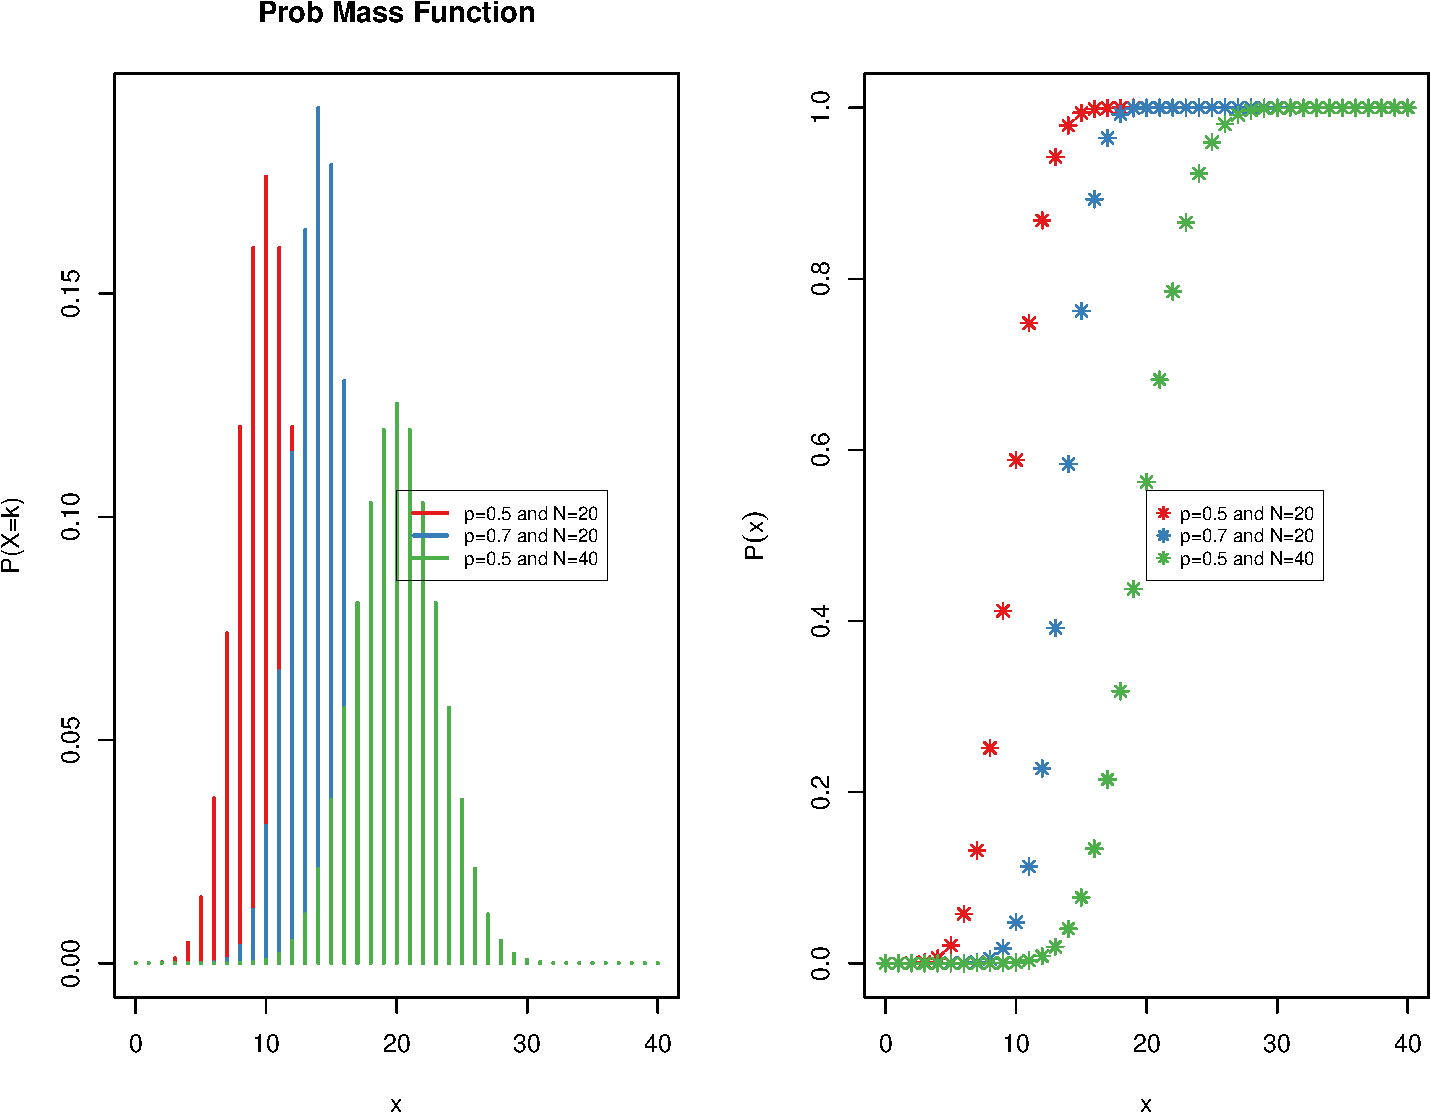
\includegraphics{index_files/figure-latex/unnamed-chunk-141-1.pdf}

with \emph{mean} \(np\) and \emph{variance} \(np(1-p)\).

\textbf{Question:}

Suppose there are twelve multiple choice questions in an Maths class
quiz. Each question has five possible answers, and only one of them is
correct. Find the probability of having four or less correct answers if
a student attempts to answer every question at random.

What is the probability of 2 or 3 questions answered correctly?

\textbf{Question:}

Suppose company \textbf{A} manufactures a product \textbf{B} which have
probability 0.005 of being defective. Suppose product B is shipped in
cartons containing 25 B items. What is the probability that a randomly
chosen carton contains exactly one defective product? What is the
probability that a randomly chosen carton contains no more than one
defective widgit?

\textbf{Solutions \href{IntroSM_sol.html}{here}}

\subsection{\texorpdfstring{Poisson distribution
\(Pois(\lambda)\)}{Poisson distribution Pois(\textbackslash{}lambda)}}\label{poisson-distribution-poislambda}

The Poisson distribution is the probability distribution of independent
event occurrences in an interval. If \(\lambda\) is the mean occurrence
per interval, then the probability of having \(k\) occurrences within a
given interval is the probability mass function given by:

\[
\mbox{Pr}(\mbox{$k$ events in interval}) = \frac{\lambda^k e^{-\lambda}}{k!}
\]

The \textbf{cumulative density function} for the Poisson cumulative
probability function is \[
P(X\leq x ~|~\lambda ) = \frac{e^{-\lambda} \lambda ^x}{x!}\quad \mbox{for $x=0,1,2,...$}
\]

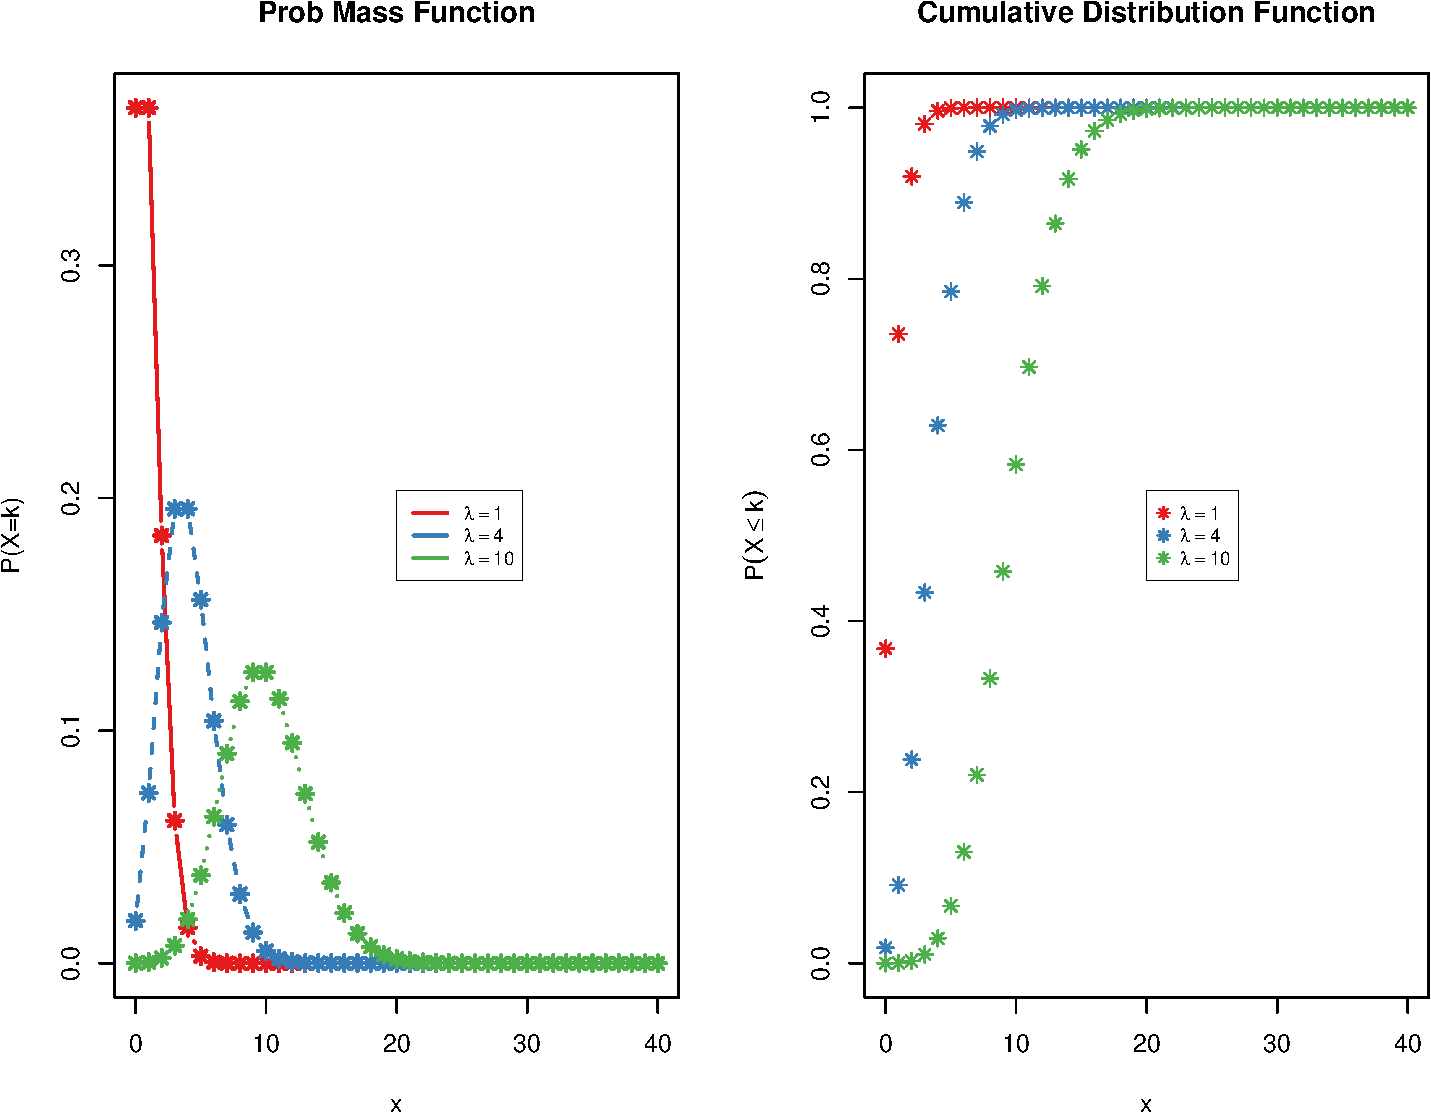
\includegraphics{index_files/figure-latex/unnamed-chunk-146-1.pdf}

\textbf{Question:}

Suppose the number of individual plants of a given species we expect to
find in a one meter square quadrat follows the Poisson distribution with
mean \(\lambda= 10\). Find the probability of finding exactly \(12\)
individuals.

\textbf{Question:}

If there are twelve cars crossing a bridge per minute on average, find
the probability of having seventeen or more cars crossing the bridge in
a particular minute.

\textbf{Solutions \href{IntroSM_sol.html}{here}}

\subsection{Aproximation of Binomial as
Poisson}\label{aproximation-of-binomial-as-poisson}

\textbf{Example}

Five percent (5\%) of Christmas tree light bulbs manufactured by a
company are defective. The company's Quality Control Manager is quite
concerned and therefore randomly samples 100 bulbs coming off of the
assembly line. Let X denote the number in the sample that are defective.
What is the probability that the sample contains at most three defective
bulbs?

\begin{Shaded}
\begin{Highlighting}[]
\NormalTok{p =}\StringTok{ }\FloatTok{0.05}
\NormalTok{k =}\StringTok{ }\DecValTok{3}
\NormalTok{n =}\StringTok{ }\DecValTok{100}
\KeywordTok{pbinom}\NormalTok{(k,}\DataTypeTok{size=}\NormalTok{n,}\DataTypeTok{prob=}\NormalTok{p)}
\end{Highlighting}
\end{Shaded}

\begin{verbatim}
## [1] 0.2578387
\end{verbatim}

It can be demonstrated that the Binomial distribution can be
approximated with the Poisson probability mass function when \(n\) is
large. Using the Poisson distribution, the mean \(\lambda = np\)

\begin{Shaded}
\begin{Highlighting}[]
\NormalTok{lambda <-}\StringTok{ }\NormalTok{n*p}
\KeywordTok{sum}\NormalTok{(}\KeywordTok{dpois}\NormalTok{(}\DecValTok{0}\NormalTok{:}\DecValTok{3}\NormalTok{,lambda))}
\end{Highlighting}
\end{Shaded}

\begin{verbatim}
## [1] 0.2650259
\end{verbatim}

It is important to keep in mind that the Poisson approximation to the
binomial distribution works well only when \(n\) is large and \(p\) is
small. In general, the approximation works well if \(n \geq 20\) and
\(p\leq0.05\), or if \(n\geq 100\) and \(p\leq 0.10\).

\subsection{\texorpdfstring{Exponential distribution
\(Exp(\lambda)\)}{Exponential distribution Exp(\textbackslash{}lambda)}}\label{exponential-distribution-explambda}

The exponential distribution is the probability distribution that
describes the time between events in a Poisson process, i.e.~a process
in which events occur continuously and independently at a constant
average rate. It is a particular case of the gamma distribution. It is
the continuous analogue of the geometric distribution, and it has the
key property of being memoryless. In addition to being used for the
analysis of Poisson processes, it is found in various other contexts.

The probability density function (pdf) of an exponential distribution as
\[
f(x;\lambda) =  \lambda \exp(-\lambda x)
\]

where \(\lambda>0\) is the event rate (also known as rate parameter,
arrival rate, death rate, failure rate, transition rate). The
exponential variable \(x \in [0,\infty)\)
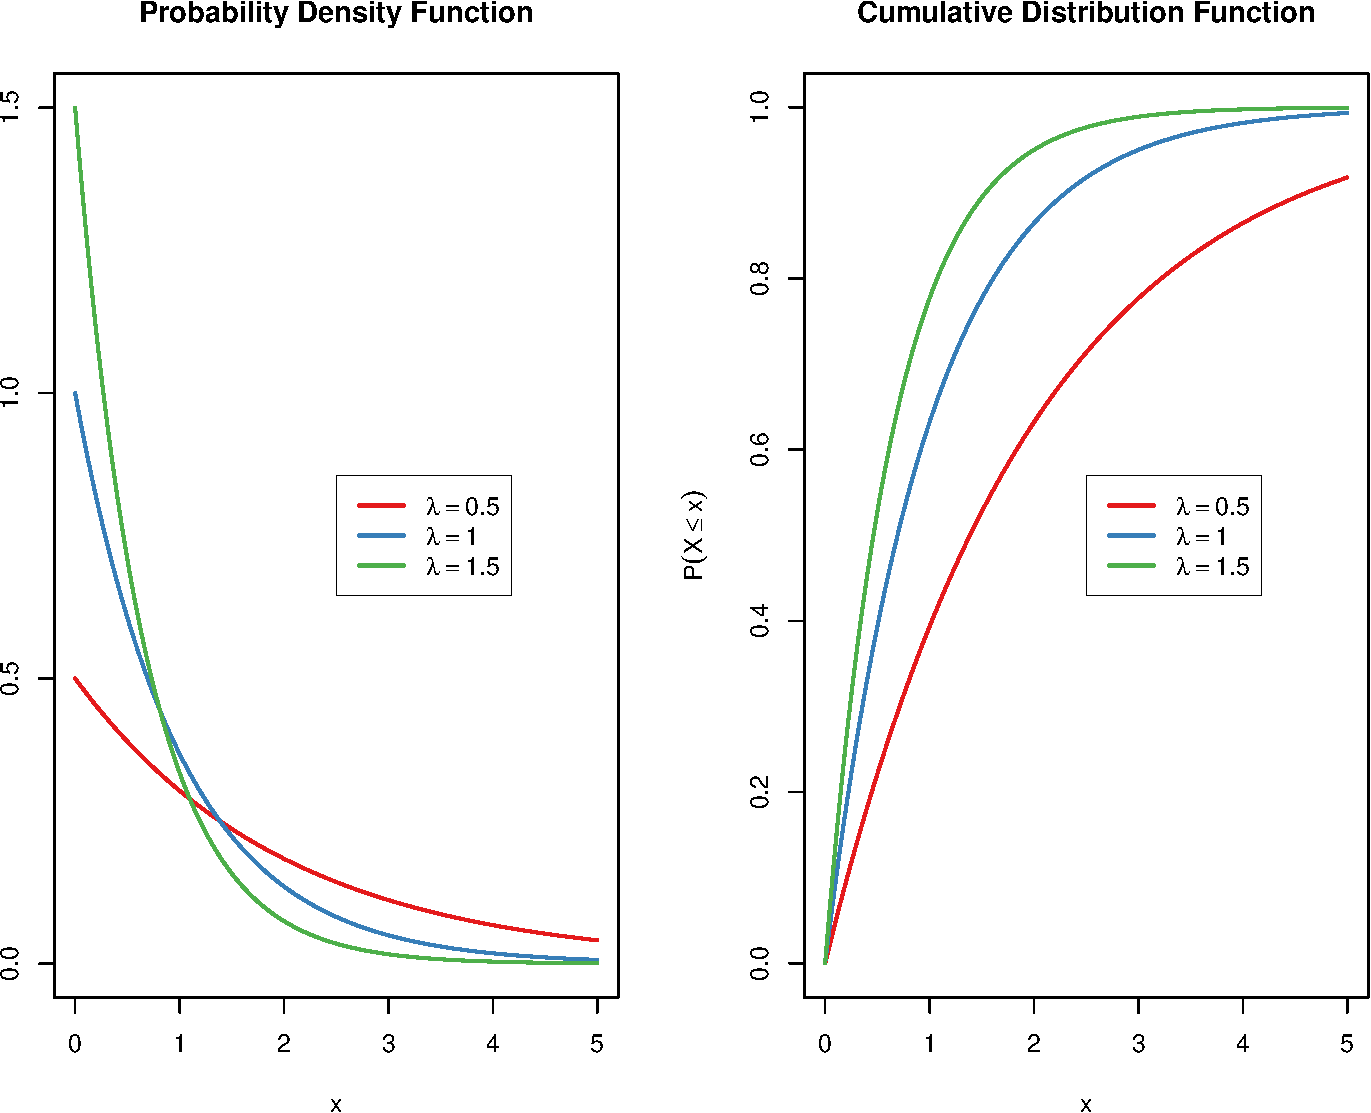
\includegraphics{index_files/figure-latex/unnamed-chunk-149-1.pdf}

Cumulative distribution function of the exponential distribution is \[
F(x) = \mbox{Pr}(X\leq x) = 
  \left\{
    \begin{array}{lcc}
      1- e^{-\lambda x} & & x\geq 0 \\
      0                 & & x < 0
    \end{array}
  \right.
\]

Mean \(\mathbb{E}(X) = 1/\lambda\), and
\(\mathbb{V}ar(X) = 1/\lambda^2\).

\textbf{Question:}

Suppose that the amount of time one spends in a bank is exponentially
distributed with mean 10 minutes, \(\lambda=1/10\).

\begin{itemize}
\tightlist
\item
  What is the probability that a customer will spend more than 15
  minutes in the bank?
\item
  What is the probability that a customer will spend more than 15
  minutes in the bank given that he is still in the bank after 10
  minutes?
\end{itemize}

\textbf{Solutions \href{IntroSM_sol.html}{here}}

\subsection{\texorpdfstring{The Normal distribution
\(\mathcal{N}(\mu,\sigma^2)\)}{The Normal distribution \textbackslash{}mathcal\{N\}(\textbackslash{}mu,\textbackslash{}sigma\^{}2)}}\label{the-normal-distribution-mathcalnmusigma2}

The probability density function of the Normal distribution is:

\[
f(x | \mu,\sigma^2) = \frac{1}{\sqrt{2\sigma^2\pi}} e ^{-\frac{(x-\mu)^2}{2\sigma^2}},
\] where

\begin{itemize}
\tightlist
\item
  \(\mu\) is the mean of the distribution (also the median and the
  mode).
\item
  \(\sigma\) is the standard deviation (\(\sigma>0\)).
\item
  \(\sigma^2\) is the variance.
\end{itemize}

The process to standardized Normal distribution consists in transforming
the Normal variable \(N(\mu,\sigma)\) to \(N(0,1)\), i.e. \[
Z = \frac{X-\mu}{\sigma} \sim N(0,1)
\]

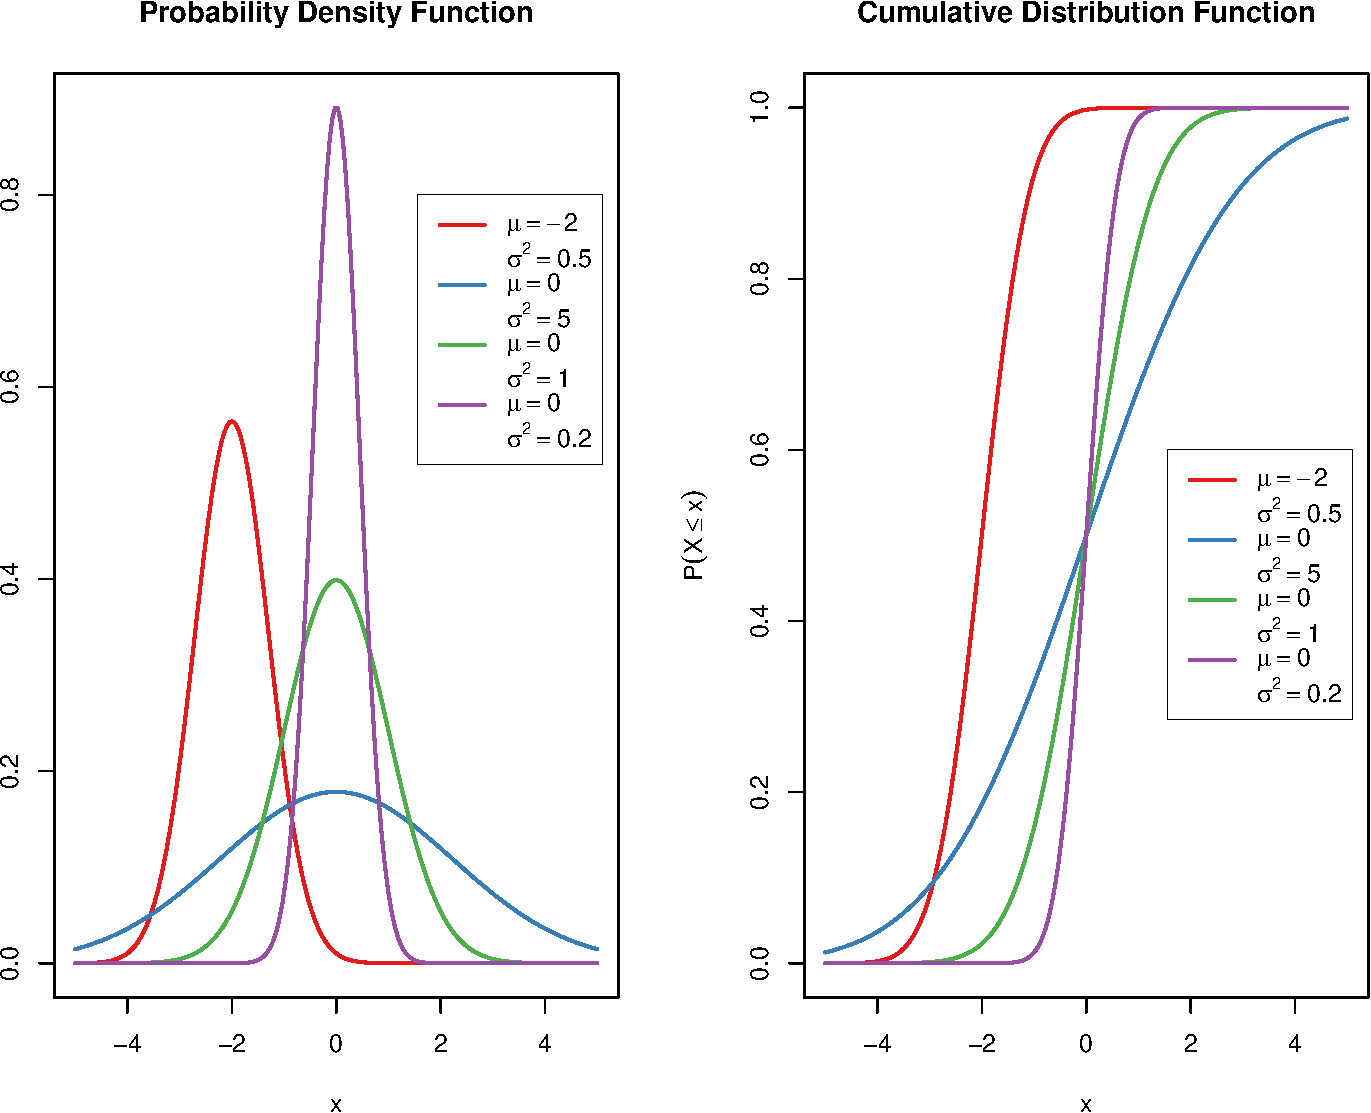
\includegraphics{index_files/figure-latex/unnamed-chunk-150-1.pdf}

\textbf{Question:}

\(X\) is a normally distributed variable with mean \(\mu = 30\) and
standard deviation \(\sigma = 4\). Find

\begin{enumerate}
\def\labelenumi{\alph{enumi})}
\item
  \(P(x<40)\)
\item
  \(P(x>21)\)
\item
  \(P(30<x<35)\)
\end{enumerate}

\textbf{Question:}

Entry to a certain University is determined by a national test. The
scores on this test are normally distributed with a mean of 500 and a
standard deviation of 100. Tom wants to be admitted to this university
and he knows that he must score better than at least 70\% of the
students who took the test. Tom takes the test and scores 585. Will he
be admitted to this university?

\textbf{Solutions \href{IntroSM_sol.html}{here}}

\subsection{Exercises}\label{exercises}

\begin{enumerate}
\def\labelenumi{\arabic{enumi}.}
\tightlist
\item
  A dice is thrown at random. What is the expectation of number on it?
  (Or) If x denotes the number of points on a dice, find the expectation
  and the variance of x.
\end{enumerate}

\begin{Shaded}
\begin{Highlighting}[]
\NormalTok{x =}\StringTok{ }\DecValTok{1}\NormalTok{:}\DecValTok{6}
\NormalTok{prob <-}\StringTok{ }\DecValTok{1}\NormalTok{/}\DecValTok{6}

 \NormalTok{E  <-}\StringTok{ }\KeywordTok{sum}\NormalTok{(x*}\KeywordTok{rep}\NormalTok{(prob,}\KeywordTok{length}\NormalTok{(x)))}
 
 \NormalTok{E2 <-}\StringTok{ }\NormalTok{E^}\DecValTok{2}
 \NormalTok{Ex2 <-}\StringTok{ }\KeywordTok{sum}\NormalTok{(x^}\DecValTok{2}\NormalTok{*}\KeywordTok{rep}\NormalTok{(prob,}\KeywordTok{length}\NormalTok{(x)))}
\NormalTok{Var <-}\StringTok{ }\NormalTok{Ex2-E2}
\end{Highlighting}
\end{Shaded}

\begin{enumerate}
\def\labelenumi{\arabic{enumi}.}
\setcounter{enumi}{1}
\tightlist
\item
  If a person gains or loses an amount equal to the number appearing
  when a balanced die is rolled once, according to whether the number is
  even or odd, how much money can be expect per game in the long run?
\end{enumerate}

Let \(x\) indicate the amount that the person wins

The amount gained by the person would be

\begin{itemize}
\tightlist
\item
  \texttt{-\ Rs.\ 1} if the dice shows up ONE
\item
  \texttt{+\ Rs.\ 2} if the dice shows up TWO
\item
  \texttt{-\ Rs.\ 3} if the dice shows up THREE
\item
  \texttt{+\ Rs.\ 4} if the dice shows up FOUR
\item
  \texttt{-\ Rs.\ 5} if the dice shows up FIVE
\item
  \texttt{+\ Rs.\ 6} if the dice shows up SIX
\end{itemize}

\begin{Shaded}
\begin{Highlighting}[]
\NormalTok{x =}\StringTok{ }\KeywordTok{c}\NormalTok{(}\DecValTok{1}\NormalTok{:}\DecValTok{6}\NormalTok{)*}\KeywordTok{c}\NormalTok{(-}\DecValTok{1}\NormalTok{,}\DecValTok{1}\NormalTok{,-}\DecValTok{1}\NormalTok{,}\DecValTok{1}\NormalTok{,-}\DecValTok{1}\NormalTok{,}\DecValTok{1}\NormalTok{)}
\NormalTok{pr <-}\StringTok{ }\KeywordTok{rep}\NormalTok{(}\DecValTok{1}\NormalTok{/}\DecValTok{6}\NormalTok{,}\DecValTok{6}\NormalTok{)}
 \NormalTok{Ex <-}\StringTok{ }\KeywordTok{sum}\NormalTok{(x*pr)}
\NormalTok{Ex2 <-}\StringTok{ }\KeywordTok{sum}\NormalTok{(x^}\DecValTok{2}\NormalTok{*pr)}
\NormalTok{Var <-}\StringTok{ }\NormalTok{Ex2-Ex^}\DecValTok{2}
\NormalTok{Ex}
\end{Highlighting}
\end{Shaded}

\begin{verbatim}
## [1] 0.5
\end{verbatim}

\begin{Shaded}
\begin{Highlighting}[]
\NormalTok{Var}
\end{Highlighting}
\end{Shaded}

\begin{verbatim}
## [1] 14.91667
\end{verbatim}

\section{Statistical Inference}\label{statistical-inference}

Statistical inference means drawing conclusions based on data. There are
many ways of performing inference including statistical modeling, data
oriented strategies and explicit use of designs and randomization in
analyses. Furthermore, there are broad theories (frequentists, Bayesian,
likelihood, design based, \ldots{}) and numerous complexities (missing
data, observed and unobserved confounding, biases) for performing
inference. This section presents the fundamentals of inference in a
practical approach for getting things done in order to use statistical
inference for making informed choices in analyzing data.

\subsection{Interval estimation}\label{interval-estimation}

It is a common requirement to efficiently estimate population parameters
based on simple random sample data.

\begin{Shaded}
\begin{Highlighting}[]
\KeywordTok{library}\NormalTok{(MASS)}
\NormalTok{?survey}
\KeywordTok{head}\NormalTok{(survey)}
\end{Highlighting}
\end{Shaded}

\begin{verbatim}
##      Sex Wr.Hnd NW.Hnd W.Hnd    Fold Pulse    Clap Exer Smoke Height
## 1 Female   18.5   18.0 Right  R on L    92    Left Some Never 173.00
## 2   Male   19.5   20.5  Left  R on L   104    Left None Regul 177.80
## 3   Male   18.0   13.3 Right  L on R    87 Neither None Occas     NA
## 4   Male   18.8   18.9 Right  R on L    NA Neither None Never 160.00
## 5   Male   20.0   20.0 Right Neither    35   Right Some Never 165.00
## 6 Female   18.0   17.7 Right  L on R    64   Right Some Never 172.72
##        M.I    Age
## 1   Metric 18.250
## 2 Imperial 17.583
## 3     <NA> 16.917
## 4   Metric 20.333
## 5   Metric 23.667
## 6 Imperial 21.000
\end{verbatim}

\textbf{Point estimate of population mean}

For any particular random sample, we can always compute its sample mean.
Although most often it is not the actual population mean, it does serve
as a good point estimate. For example, in the data set survey, the
survey is performed on a sample of the student population. We can
compute the sample mean and use it as an estimate of the corresponding
population parameter.

\textbf{Problem:} Find a point estimate of mean university student
height with the sample data from survey.

\begin{Shaded}
\begin{Highlighting}[]
\KeywordTok{mean}\NormalTok{(survey$Height)}
\end{Highlighting}
\end{Shaded}

\begin{verbatim}
## [1] NA
\end{verbatim}

\begin{Shaded}
\begin{Highlighting}[]
\KeywordTok{mean}\NormalTok{(survey$Height,}\DataTypeTok{na.rm=}\OtherTok{TRUE}\NormalTok{) }
\end{Highlighting}
\end{Shaded}

\begin{verbatim}
## [1] 172.3809
\end{verbatim}

\begin{Shaded}
\begin{Highlighting}[]
\CommentTok{# or}
\KeywordTok{mean}\NormalTok{(}\KeywordTok{na.omit}\NormalTok{(survey$Height))}
\end{Highlighting}
\end{Shaded}

\begin{verbatim}
## [1] 172.3809
\end{verbatim}

After we found a point estimate of the population mean, we would need a
way to quantify its accuracy.

\subsubsection{Interval Estimate of Population Mean (with known
variance)}\label{interval-estimate-of-population-mean-with-known-variance}

Let us denote the \(100~(1-\alpha/2)\) percentile of the standard normal
distribution as \(z_{\alpha/2}\). For random sample of sufficiently
large size, the end points of the interval estimate at \((1-\alpha/2)\)
confidence level is given as follows: \[
  \bar{x} \pm \frac{\sigma}{\sqrt{n}}
\]

\textbf{Problem:} assume the population standard deviation \(\sigma\) of
the student height in survey is 9.48. Find the margin of error and
interval estimate at 95\% confidence level.

\begin{Shaded}
\begin{Highlighting}[]
\NormalTok{x <-}\StringTok{ }\KeywordTok{na.omit}\NormalTok{(survey$Height)}
\NormalTok{n <-}\StringTok{ }\KeywordTok{length}\NormalTok{(x)}
\NormalTok{sigma <-}\StringTok{ }\FloatTok{9.48}
\NormalTok{sem =}\StringTok{ }\NormalTok{sigma/}\KeywordTok{sqrt}\NormalTok{(n)  }\CommentTok{# Standard error of the mean}
\NormalTok{sem}
\end{Highlighting}
\end{Shaded}

\begin{verbatim}
## [1] 0.6557453
\end{verbatim}

Since there are two tails of the normal distribution, the 95\%
confidence level would imply the 97.5th percentile of the normal
distribution at the upper tail. Therefore, \(z_{\alpha/2}\) is given by
\texttt{qnorm(.975)}. We multiply it with the standard error of the mean
\texttt{sem} and get the margin of error.

\begin{Shaded}
\begin{Highlighting}[]
\NormalTok{E <-}\StringTok{ }\KeywordTok{qnorm}\NormalTok{(}\FloatTok{0.975}\NormalTok{)*sem }
\NormalTok{E  }\CommentTok{# margin of error}
\end{Highlighting}
\end{Shaded}

\begin{verbatim}
## [1] 1.285237
\end{verbatim}

\begin{Shaded}
\begin{Highlighting}[]
\NormalTok{xbar <-}\StringTok{ }\KeywordTok{mean}\NormalTok{(x,}\DataTypeTok{na.rm =} \OtherTok{TRUE}\NormalTok{)}
\NormalTok{xbar +}\StringTok{ }\KeywordTok{c}\NormalTok{(-E,E)}
\end{Highlighting}
\end{Shaded}

\begin{verbatim}
## [1] 171.0956 173.6661
\end{verbatim}

Alternatively, we can use \texttt{z.test}

\begin{Shaded}
\begin{Highlighting}[]
\KeywordTok{library}\NormalTok{(TeachingDemos)}
\KeywordTok{z.test}\NormalTok{(x,}\DataTypeTok{sd=}\NormalTok{sigma)}
\end{Highlighting}
\end{Shaded}

\begin{verbatim}
## 
##  One Sample z-test
## 
## data:  x
## z = 262.88, n = 209.00000, Std. Dev. = 9.48000, Std. Dev. of the
## sample mean = 0.65575, p-value < 2.2e-16
## alternative hypothesis: true mean is not equal to 0
## 95 percent confidence interval:
##  171.0956 173.6661
## sample estimates:
## mean of x 
##  172.3809
\end{verbatim}

Assuming the population standard deviation \(\sigma\) being 9.48, the
margin of error for the student height survey at 95\% confidence level
is 1.2852372 centimeters. The confidence interval is between 171.095624
and 173.6660984 centimeters.

\subsubsection{Interval Estimate of Population Mean (with unknown
variance)}\label{interval-estimate-of-population-mean-with-unknown-variance}

\begin{Shaded}
\begin{Highlighting}[]
\NormalTok{s =}\StringTok{ }\KeywordTok{sd}\NormalTok{(x)}
\NormalTok{SE <-}\StringTok{ }\NormalTok{s/}\KeywordTok{sqrt}\NormalTok{(n)}
\NormalTok{E =}\StringTok{ }\KeywordTok{qt}\NormalTok{(.}\DecValTok{975}\NormalTok{, }\DataTypeTok{df=}\NormalTok{n}\DecValTok{-1}\NormalTok{)*SE; E}
\end{Highlighting}
\end{Shaded}

\begin{verbatim}
## [1] 1.342878
\end{verbatim}

\begin{Shaded}
\begin{Highlighting}[]
\NormalTok{xbar +}\StringTok{ }\KeywordTok{c}\NormalTok{(-E, E) }
\end{Highlighting}
\end{Shaded}

\begin{verbatim}
## [1] 171.0380 173.7237
\end{verbatim}

\begin{Shaded}
\begin{Highlighting}[]
\CommentTok{# or }

\KeywordTok{t.test}\NormalTok{(x)}
\end{Highlighting}
\end{Shaded}

\begin{verbatim}
## 
##  One Sample t-test
## 
## data:  x
## t = 253.07, df = 208, p-value < 2.2e-16
## alternative hypothesis: true mean is not equal to 0
## 95 percent confidence interval:
##  171.0380 173.7237
## sample estimates:
## mean of x 
##  172.3809
\end{verbatim}

Without assumption on the population standard deviation, the margin of
error for the student height survey at 95\% confidence level is 1.3429
centimeters. The confidence interval is between 171.04 and 173.72
centimeters.

\paragraph{Sampling Size of Population
Mean}\label{sampling-size-of-population-mean}

The quality of a sample survey can be improved by increasing the sample
size. The formula below provide the sample size needed under the
requirement of population mean interval estimate at \((1-\alpha)\)
confidence level, margin of error \(E\), and population variance
\(\sigma^2\). Here, \(z_{\alpha-2}\) is the \(100(1 -\alpha/2)\)
percentile of the standard normal distribution.

\[
    n = \frac{(z_{\alpha/2})^2 \sigma^2}{E^2}
\]

\textbf{Problem:}

Assume the population standard deviation \(\sigma\) of the student
height in \texttt{survey} is 9.48. Find the sample size needed to
achieve a 1.2 centimeters margin of error at 95\% confidence level.

\begin{Shaded}
\begin{Highlighting}[]
\NormalTok{zstar =}\StringTok{ }\KeywordTok{qnorm}\NormalTok{(.}\DecValTok{975}\NormalTok{) }
\NormalTok{sigma =}\StringTok{ }\FloatTok{9.48} 
\NormalTok{E =}\StringTok{ }\FloatTok{1.2} 
\NormalTok{zstar^}\DecValTok{2} \NormalTok{*sigma^}\DecValTok{2}\NormalTok{/}\StringTok{ }\NormalTok{E^}\DecValTok{2} 
\end{Highlighting}
\end{Shaded}

\begin{verbatim}
## [1] 239.7454
\end{verbatim}

Based on the assumption of population standard deviation being 9.48, it
needs a sample size of 240 to achieve a 1.2 centimeters margin of error
at 95\% confidence level.

\subsubsection{Interval estimates of population
proportion}\label{interval-estimates-of-population-proportion}

\textbf{Point estimate of population proportion}

Multiple choice questionnaires in a survey are often used to determine
the the proportion of a population with certain characteristic. For
example, we can estimate the proportion of female students in the
university based on the result in the sample data set \texttt{survey}.

\textbf{Problem:} Find a point estimate of the female student proportion
from survey.

\begin{Shaded}
\begin{Highlighting}[]
\KeywordTok{library}\NormalTok{(MASS)}
\NormalTok{gender.response <-}\StringTok{ }\KeywordTok{na.omit}\NormalTok{(survey$Sex) }\CommentTok{# filter out NA's}
\NormalTok{n <-}\StringTok{ }\KeywordTok{length}\NormalTok{(gender.response)}
\KeywordTok{table}\NormalTok{(gender.response)}
\end{Highlighting}
\end{Shaded}

\begin{verbatim}
## gender.response
## Female   Male 
##    118    118
\end{verbatim}

To find out the number of female students, we compare
\texttt{gender.response}

\begin{Shaded}
\begin{Highlighting}[]
\NormalTok{k <-}\StringTok{ }\KeywordTok{sum}\NormalTok{(gender.response ==}\StringTok{ "Female"}\NormalTok{) }
\CommentTok{# or }
\NormalTok{k <-}\StringTok{ }\KeywordTok{table}\NormalTok{(gender.response)[}\DecValTok{1}\NormalTok{]}

\NormalTok{pbar <-}\StringTok{ }\NormalTok{k/n; pbar}
\end{Highlighting}
\end{Shaded}

\begin{verbatim}
## Female 
##    0.5
\end{verbatim}

The point estimate of the female student proportion in survey is 50\%.

In order to compute the confidence interval of the estimated proportion,
let us denote the \(100(1-\alpha/2)\) percentile of the standard normal
distribution as \(z_{\alpha/2}\). If the samples size \(n\) and
population proportion \(p\) satisfy the condition that \(np \geq 5\) and
\(n(1-p) \geq 5\), than the end points of the interval estimate at
\((1-\alpha)\) confidence level is defined in terms of the sample
proportion as follows.

\[
      \bar{p} = \pm z_{\alpha/2} \sqrt{\frac{\bar{p}(1-\bar{p})}{n}} 
\]

We use the \texttt{prop.test} function for direct calculation

\begin{Shaded}
\begin{Highlighting}[]
\KeywordTok{prop.test}\NormalTok{(k,n,}\DataTypeTok{conf.level =} \FloatTok{0.95}\NormalTok{)}
\end{Highlighting}
\end{Shaded}

\begin{verbatim}
## 
##  1-sample proportions test without continuity correction
## 
## data:  k out of n, null probability 0.5
## X-squared = 0, df = 1, p-value = 1
## alternative hypothesis: true p is not equal to 0.5
## 95 percent confidence interval:
##  0.4367215 0.5632785
## sample estimates:
##   p 
## 0.5
\end{verbatim}

At 95\% confidence level, between 43.6\% and 56.3\% of the university
students are female, and the margin of error is 6.4\%.

\paragraph{Sampling Size of Population
proportion}\label{sampling-size-of-population-proportion}

The quality of a sample survey can be improved by increasing the sample
size. The formula below provide the sample size needed under the
requirement of population proportion interval estimate at
\((1 -\alpha)\) confidence level, margin of error \(E\), and planned
proportion estimate \(p\). Here, \(z_{\alpha/2}\) is the
\(100(1-\alpha/2)\) percentile of the standard normal distribution.

\[
   n  = \frac{(z_{\alpha/2})^2 p (1-p)}{E^2}
\]

\begin{Shaded}
\begin{Highlighting}[]
\NormalTok{zstar =}\StringTok{ }\KeywordTok{qnorm}\NormalTok{(.}\DecValTok{975}\NormalTok{) }
\NormalTok{p =}\StringTok{ }\FloatTok{0.5} 
\NormalTok{E =}\StringTok{ }\FloatTok{0.05} 
\NormalTok{zstar^}\DecValTok{2} \NormalTok{*}\StringTok{ }\NormalTok{p *}\StringTok{ }\NormalTok{(}\DecValTok{1}\NormalTok{-p) /}\StringTok{ }\NormalTok{E^}\DecValTok{2} 
\end{Highlighting}
\end{Shaded}

\begin{verbatim}
## [1] 384.1459
\end{verbatim}

With a planned proportion estimate of 50\% at 95\% confidence level, it
needs a sample size of 385 to achieve a 5\% margin of error for the
survey of female student proportion.

\subsection{Inference about two
populations}\label{inference-about-two-populations}

It is often necessary to draw conclusion on the difference between two
populations by their data samples. In the following tutorials, we
discuss how to estimate the difference of means and proportions between
two normally distributed data populations.

\subsubsection{Population mean between two matches
samples}\label{population-mean-between-two-matches-samples}

Two data samples are matched if they come from repeated observations of
the same subject. Here, we assume that the data populations follow the
normal distribution. Using the paired t-test, we can obtain an interval
estimate of the difference of the population means.

\begin{Shaded}
\begin{Highlighting}[]
\KeywordTok{library}\NormalTok{(MASS)}
\KeywordTok{data}\NormalTok{(immer)}
\NormalTok{?immer}
\KeywordTok{head}\NormalTok{(immer)}
\end{Highlighting}
\end{Shaded}

\begin{verbatim}
##   Loc Var    Y1    Y2
## 1  UF   M  81.0  80.7
## 2  UF   S 105.4  82.3
## 3  UF   V 119.7  80.4
## 4  UF   T 109.7  87.2
## 5  UF   P  98.3  84.2
## 6   W   M 146.6 100.4
\end{verbatim}

\textbf{Problem:}

Assuming that the data in \texttt{immer} follows the normal
distribution, find the 95\% confidence interval estimate of the
difference between the mean barley yields between years 1931 and 1932.

\begin{Shaded}
\begin{Highlighting}[]
\KeywordTok{t.test}\NormalTok{(immer$Y1, immer$Y2, }\DataTypeTok{paired=}\OtherTok{TRUE}\NormalTok{) }
\end{Highlighting}
\end{Shaded}

\begin{verbatim}
## 
##  Paired t-test
## 
## data:  immer$Y1 and immer$Y2
## t = 3.324, df = 29, p-value = 0.002413
## alternative hypothesis: true difference in means is not equal to 0
## 95 percent confidence interval:
##   6.121954 25.704713
## sample estimates:
## mean of the differences 
##                15.91333
\end{verbatim}

\textbf{Answer:}

Between years 1931 and 1932 in the data set \texttt{immer}, the 95\%
confidence interval of the difference in means of the barley yields is
the interval between 6.122 and 25.705.

\hypertarget{population-mean-between-two-independent-samples}{\subsection{Population
Mean Between Two Independent
Samples}\label{population-mean-between-two-independent-samples}}

Two data samples are independent if they come from unrelated populations
and the samples does not affect each other. Here, we assume that the
data populations follow the normal distribution. Using the unpaired
t-test, we can obtain an interval estimate of the difference between two
population means.

\emph{Example:}

In the data frame column mpg of the data set \texttt{mtcars}, there are
gas mileage data of various 1974 U.S. automobiles. \texttt{am} variable
indicates the transmission type of the automobile model (0 = automatic,
1 = manual).

In particular, the gas mileage for manual and automatic transmissions
are two independent data populations.

\textbf{Problem:}

Assuming that the data in \texttt{mtcars} follows the normal
distribution, find the 95\% confidence interval estimate of the
difference between the mean gas mileage of manual and automatic
transmissions.

\begin{Shaded}
\begin{Highlighting}[]
\KeywordTok{t.test}\NormalTok{(mpg ~}\StringTok{ }\NormalTok{am, }\DataTypeTok{data=}\NormalTok{mtcars) }
\end{Highlighting}
\end{Shaded}

\begin{verbatim}
## 
##  Welch Two Sample t-test
## 
## data:  mpg by am
## t = -3.7671, df = 18.332, p-value = 0.001374
## alternative hypothesis: true difference in means is not equal to 0
## 95 percent confidence interval:
##  -11.280194  -3.209684
## sample estimates:
## mean in group 0 mean in group 1 
##        17.14737        24.39231
\end{verbatim}

In \texttt{mtcars}, the mean mileage of automatic transmission is 17.147
\texttt{mpg} and the manual transmission is 24.392 \texttt{mpg}. The
95\% confidence interval of the difference in mean gas mileage is
between 3.2097 and 11.2802 \texttt{mpg}.

\subsection{Comparison of Two Population
Proportions}\label{comparison-of-two-population-proportions}

A survey conducted in two distinct populations will produce different
results. It is often necessary to compare the survey response proportion
between the two populations. Here, we assume that the data populations
follow the normal distribution.

\textbf{Example:}

In the built-in data set named quine, children from an Australian town
is classified by ethnic background, gender, age, learning status and the
number of days absent from school.

\begin{Shaded}
\begin{Highlighting}[]
\KeywordTok{library}\NormalTok{(MASS)}
\KeywordTok{data}\NormalTok{(quine)}
\NormalTok{?quine}
\KeywordTok{head}\NormalTok{(quine)}
\end{Highlighting}
\end{Shaded}

\begin{verbatim}
##   Eth Sex Age Lrn Days
## 1   A   M  F0  SL    2
## 2   A   M  F0  SL   11
## 3   A   M  F0  SL   14
## 4   A   M  F0  AL    5
## 5   A   M  F0  AL    5
## 6   A   M  F0  AL   13
\end{verbatim}

Column \texttt{Eth} indicates whether the student is Aboriginal or Not
(``A'' or ``N''), and the column \texttt{Sex} indicates Male or Female
(``M'' or ``F'').

\begin{Shaded}
\begin{Highlighting}[]
\KeywordTok{table}\NormalTok{(quine$Eth,quine$Sex)}
\end{Highlighting}
\end{Shaded}

\begin{verbatim}
##    
##      F  M
##   A 38 31
##   N 42 35
\end{verbatim}

\textbf{Problem:}

Assuming that the data in quine follows the normal distribution, find
the 95\% confidence interval estimate of the difference between the
female proportion of Aboriginal students and the female proportion of
Non-Aboriginal students, each within their own ethnic group.

\textbf{Solution}

We apply the `prop.test function to compute the difference in female
proportions. The Yates's continuity correction is disabled for
pedagogical reasons.

\begin{Shaded}
\begin{Highlighting}[]
\KeywordTok{prop.test}\NormalTok{(}\KeywordTok{table}\NormalTok{(quine$Eth, quine$Sex), }\DataTypeTok{correct=}\OtherTok{FALSE}\NormalTok{) }
\end{Highlighting}
\end{Shaded}

\begin{verbatim}
## 
##  2-sample test for equality of proportions without continuity
##  correction
## 
## data:  table(quine$Eth, quine$Sex)
## X-squared = 0.0040803, df = 1, p-value = 0.9491
## alternative hypothesis: two.sided
## 95 percent confidence interval:
##  -0.1564218  0.1669620
## sample estimates:
##    prop 1    prop 2 
## 0.5507246 0.5454545
\end{verbatim}

The 95\% confidence interval estimate of the difference between the
female proportion of Aboriginal students and the female proportion of
Non-Aboriginal students is between -15.6\% and 16.7\%.

\subsection{Goodness-of-Fit}\label{goodness-of-fit}

Many statistical quantities derived from data samples are found to
follow the Chi-squared distribution. Hence we can use it to test whether
a population fits a particular theoretical probability distribution.

\subsection{Chi-squared Test of
Independence}\label{chi-squared-test-of-independence}

Two random variables \(x\) and \(y\) are called independent if the
probability distribution of one variable is not affected by the presence
of another. Assume \(f_{ij}\) is the observed frequency count of events
belonging to both \(i\)-th category of x and \(j\)-th category of \(y\).
Also assume \(e_{ij}\) to be the corresponding expected count if \(x\)
and \(y\) are independent. The null hypothesis of the independence
assumption is to be rejected if the p-value of the following Chi-squared
test statistics is less than a given significance level \(\alpha\).

\[
  \chi^2 = \sum_{i,j}\frac{(f_i - e_i)^2}{e_i}
\]

\textbf{Example:}

In the built-in data set \texttt{survey}, the \texttt{Smoke} column
records the students smoking habit, while the \texttt{Exer} column
records their exercise level. The allowed values in Smoke are ``Heavy'',
``Regul'' (regularly), ``Occas'' (occasionally) and ``Never''. As for
Exer, they are ``Freq'' (frequently), ``Some'' and ``None''.

\begin{Shaded}
\begin{Highlighting}[]
\KeywordTok{library}\NormalTok{(MASS)}
\KeywordTok{data}\NormalTok{(survey)}
\NormalTok{tbl <-}\StringTok{ }\KeywordTok{table}\NormalTok{(survey$Smoke,survey$Exer)}
\NormalTok{tbl}
\end{Highlighting}
\end{Shaded}

\begin{verbatim}
##        
##         Freq None Some
##   Heavy    7    1    3
##   Never   87   18   84
##   Occas   12    3    4
##   Regul    9    1    7
\end{verbatim}

\textbf{Problem:}

Test the hypothesis whether the students smoking habit is independent of
their exercise level at \(0.05\) significance level.

\begin{Shaded}
\begin{Highlighting}[]
\NormalTok{chi2test <-}\StringTok{ }\KeywordTok{chisq.test}\NormalTok{(tbl) }
\NormalTok{chi2test}
\end{Highlighting}
\end{Shaded}

\begin{verbatim}
## 
##  Pearson's Chi-squared test
## 
## data:  tbl
## X-squared = 5.4885, df = 6, p-value = 0.4828
\end{verbatim}

As the p-value is 0.4828422 greater than the 0.05 significance level, we
do not reject the null hypothesis that the smoking habit is independent
of the exercise level of the students.

The warning message found in the solution above is due to the small cell
values in the contingency table. To avoid such warning, we combine the
second and third columns of \texttt{tbl}, and save it in a new table
named \texttt{ctbl}. Then we apply the \texttt{chisq.test} function
against \texttt{ctbl} instead.

\begin{Shaded}
\begin{Highlighting}[]
\NormalTok{ctbl <-}\StringTok{ }\KeywordTok{cbind}\NormalTok{(tbl[,}\StringTok{"Freq"}\NormalTok{], tbl[,}\StringTok{"None"}\NormalTok{] +}\StringTok{ }\NormalTok{tbl[,}\StringTok{"Some"}\NormalTok{])}
\NormalTok{ctbl}
\end{Highlighting}
\end{Shaded}

\begin{verbatim}
##       [,1] [,2]
## Heavy    7    4
## Never   87  102
## Occas   12    7
## Regul    9    8
\end{verbatim}

\begin{Shaded}
\begin{Highlighting}[]
\NormalTok{chi2test <-}\StringTok{ }\KeywordTok{chisq.test}\NormalTok{(ctbl)}
\NormalTok{chi2test}
\end{Highlighting}
\end{Shaded}

\begin{verbatim}
## 
##  Pearson's Chi-squared test
## 
## data:  ctbl
## X-squared = 3.2328, df = 3, p-value = 0.3571
\end{verbatim}

The p-value is 0.3571031 also greater than the 0.05 significance level.

\subsection{Mann-Whitney U test}\label{mann-whitney-u-test}

Also known as Mann-Whitney-Wilcoxon (MWW), Wilcoxon rank-sum test, or
Wilcoxon-Mann-Whitney test is a non-parametric test of the null
hypothesis that two samples come from the same sample population against
an alternative hypothesis, especially that a particular population tends
to have larger values than the other. Is the alternative test to the
independent sample t-test. As a non-parametric test, it does not assume
any assumptions related to the distribution. Hence, we can decide
whether the population distributions are identical without assuming them
to follow the normal distribution.

There are, however, some assumptions that are assumed:

\begin{enumerate}
\def\labelenumi{\arabic{enumi}.}
\tightlist
\item
  The sample drawn from the population is random.
\item
  Independence within the samples and mutual independence is assumed.
\item
  Ordinal measurement scale is assumed.
\end{enumerate}

Mann-Whitney U test is used for every field, but in frequently used in
psychology, medical/nursing and business. For example, in psychology, it
is used to compare attitude or behavior, etc. In medicine, it is used to
know the effect of two medicines and whether they are equal or not. It
is also used to know whether or not a particular medicine cures the
ailment or not. In business, it can be used to know the preferences of
different people and it can be used to see if that changes depending on
location.

\textbf{Example} Consider the \texttt{mtcars} data set. We are aim to
find out whether automatic transmission cars are less fuel efficient
compared to manual transmission cars. Since 1950, most cars sold in
North America have been available with an automatic transmission.

The \texttt{mtcars} dataset is from the 1974 ``Motor Trend US''
magazine, consisting of fuel consumption measurement (mpg) and 10
different aspects of automoblie design and performance for 32
automobiles (1973-74 models).

We first plot the data (mpg vs transmission)

either with a boxplot

\begin{Shaded}
\begin{Highlighting}[]
\KeywordTok{boxplot}\NormalTok{(mpg~am,}\DataTypeTok{data=}\NormalTok{mtcars,}\DataTypeTok{names=}\KeywordTok{c}\NormalTok{(}\StringTok{"automatic"}\NormalTok{,}\StringTok{"manual"}\NormalTok{),}\DataTypeTok{ylab=}\StringTok{"mpg"}\NormalTok{,}\DataTypeTok{xlab=}\StringTok{"Transmission"}\NormalTok{)}
\end{Highlighting}
\end{Shaded}

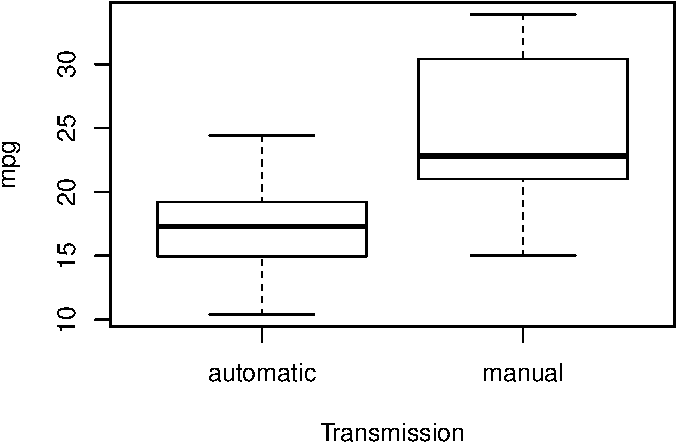
\includegraphics{index_files/figure-latex/unnamed-chunk-173-1.pdf}

or with a bar chart (with error bars)

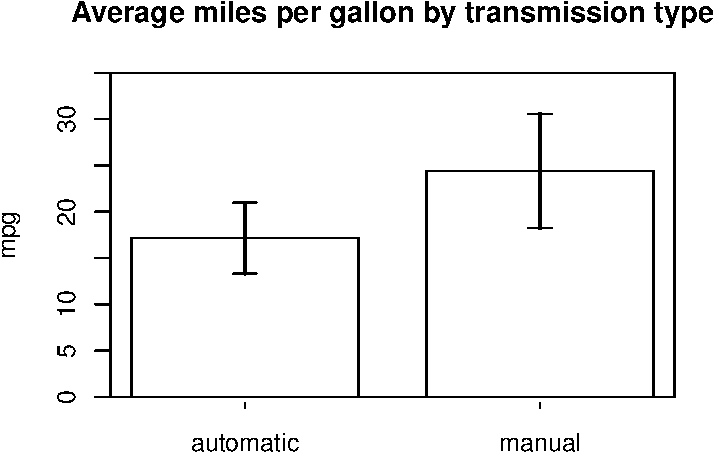
\includegraphics{index_files/figure-latex/unnamed-chunk-174-1.pdf}

We run some statistical tests to compare mpg between automatic- and
manual-transmitted cars.

The first one is a t-test, assuming that the mileage data have a normal
distribution. The test result clearly shows that the manual transmission
cars are more gas-efficient than automatic transmission cars (miles per
gallon: 24.39 versus 17.15).

\begin{Shaded}
\begin{Highlighting}[]
\KeywordTok{t.test}\NormalTok{(mpg ~}\StringTok{ }\KeywordTok{factor}\NormalTok{(am), }\DataTypeTok{data =} \NormalTok{mtcars)}
\end{Highlighting}
\end{Shaded}

\begin{verbatim}
## 
##  Welch Two Sample t-test
## 
## data:  mpg by factor(am)
## t = -3.7671, df = 18.332, p-value = 0.001374
## alternative hypothesis: true difference in means is not equal to 0
## 95 percent confidence interval:
##  -11.280194  -3.209684
## sample estimates:
## mean in group 0 mean in group 1 
##        17.14737        24.39231
\end{verbatim}

However, the normality assumption could be quite strong, given the fact
that we do not know the true underlying distributions of \texttt{mpg}
data. Moreover, the number of data points are not large enough to apply
the central limit theorem. Therefore, a more conservative test would be
the Wilcoxon test, with the null hypothesis that the gas mileage data of
manual and automatic transmissions are from identical populations.

\begin{Shaded}
\begin{Highlighting}[]
\KeywordTok{wilcox.test}\NormalTok{(mpg ~}\StringTok{ }\NormalTok{am, }\DataTypeTok{data =} \NormalTok{mtcars)}
\end{Highlighting}
\end{Shaded}

\begin{verbatim}
## Warning in wilcox.test.default(x = c(21.4, 18.7, 18.1, 14.3, 24.4, 22.8, :
## cannot compute exact p-value with ties
\end{verbatim}

\begin{verbatim}
## 
##  Wilcoxon rank sum test with continuity correction
## 
## data:  mpg by am
## W = 42, p-value = 0.001871
## alternative hypothesis: true location shift is not equal to 0
\end{verbatim}

A non-parametric, Wilcoxon test also rejects the null hypothesis that
the mileage data of the manual and automatic transmissions are from the
same population (indicating a difference).

\section{\texorpdfstring{Linear models in
\texttt{R}}{Linear models in R}}\label{linear-models-in-r}

\subsection{Simple linear regression}\label{simple-linear-regression}

\begin{itemize}
\item
  Regression is a statistical method used to predict the value of a
  response variable based on the values of a set of explanatory
  variables.
\item
  One very general form for the model would be
\end{itemize}

\[
      y = f(x_1,x_2,...,x_p) + \epsilon,
\]

where \(f\) is some unknown function and \(\epsilon\) is the error in
this representation. Since we usually don't have enough data to try to
estimate \(f\) directly (\emph{inverse problem}), we usually have to
assume that it has some restricted form.

\begin{itemize}
\item
  Any statistical model attempts to approximate the response variable or
  dependent variable \(y\) as a mathematical function of the explanatory
  variables or regressors \(X\) (also called covariates or independent
  variables).
\item
  The simplest and most common form is the \textbf{linear model (LM)}
\end{itemize}

\[
    y = \beta_0 + \beta_1 x_1 + \beta_2 x_z + \epsilon,
\] where \(\beta_i\) \(i=0,1,2\) are \emph{unknown} parameters.
\(\beta_0\) is called the intercept term. Hence, the problem is reduced
to the estimation of four values rather than the complicated infinite
dimensional \(f\).

\begin{itemize}
\tightlist
\item
  A simple linear model with a single exploratory variable is defined
  as: \[
       \hat{y} = \beta_0 + \beta_1 x
  \]
\end{itemize}

where \(\hat y\) is the fitted values for \(\beta_0\) (intercept) and
\(\beta_1\) (slope). Then for a given \(x_i\) we obtain a \(\hat{y}_i\)
that approximates \(y_i\)

Let us create a toy example (with \(p=1\)):

\begin{Shaded}
\begin{Highlighting}[]
\KeywordTok{set.seed}\NormalTok{(}\DecValTok{1}\NormalTok{)}
\NormalTok{n <-}\StringTok{ }\DecValTok{50} 

\NormalTok{x <-}\StringTok{ }\KeywordTok{seq}\NormalTok{(}\DecValTok{1}\NormalTok{,n)}
 \NormalTok{beta0 <-}\StringTok{ }\DecValTok{15}
 \NormalTok{beta1 <-}\StringTok{ }\FloatTok{0.5}

\NormalTok{sigma <-}\StringTok{ }\DecValTok{3} \CommentTok{# standar deviation of the errors}
\NormalTok{eps <-}\StringTok{ }\KeywordTok{rnorm}\NormalTok{(n,}\DataTypeTok{mean=}\DecValTok{0}\NormalTok{,}\DataTypeTok{sd=}\DecValTok{3}\NormalTok{) }\CommentTok{# generate gaussian random errors}

\CommentTok{# Generate random data}
 \NormalTok{y <-}\StringTok{ }\NormalTok{beta0 +}\StringTok{ }\NormalTok{beta1*x  +}\StringTok{  }\NormalTok{eps}
\end{Highlighting}
\end{Shaded}

Plot the data

\begin{Shaded}
\begin{Highlighting}[]
\KeywordTok{plot}\NormalTok{(x,y,}\DataTypeTok{ylim =} \KeywordTok{c}\NormalTok{(}\DecValTok{8}\NormalTok{,}\DecValTok{45}\NormalTok{), }\DataTypeTok{cex=}\FloatTok{1.3}\NormalTok{, }\DataTypeTok{xlab =} \StringTok{"x"}\NormalTok{, }\DataTypeTok{ylab=}\StringTok{"y"}\NormalTok{,}\DataTypeTok{pch=}\DecValTok{19}\NormalTok{)}
\end{Highlighting}
\end{Shaded}

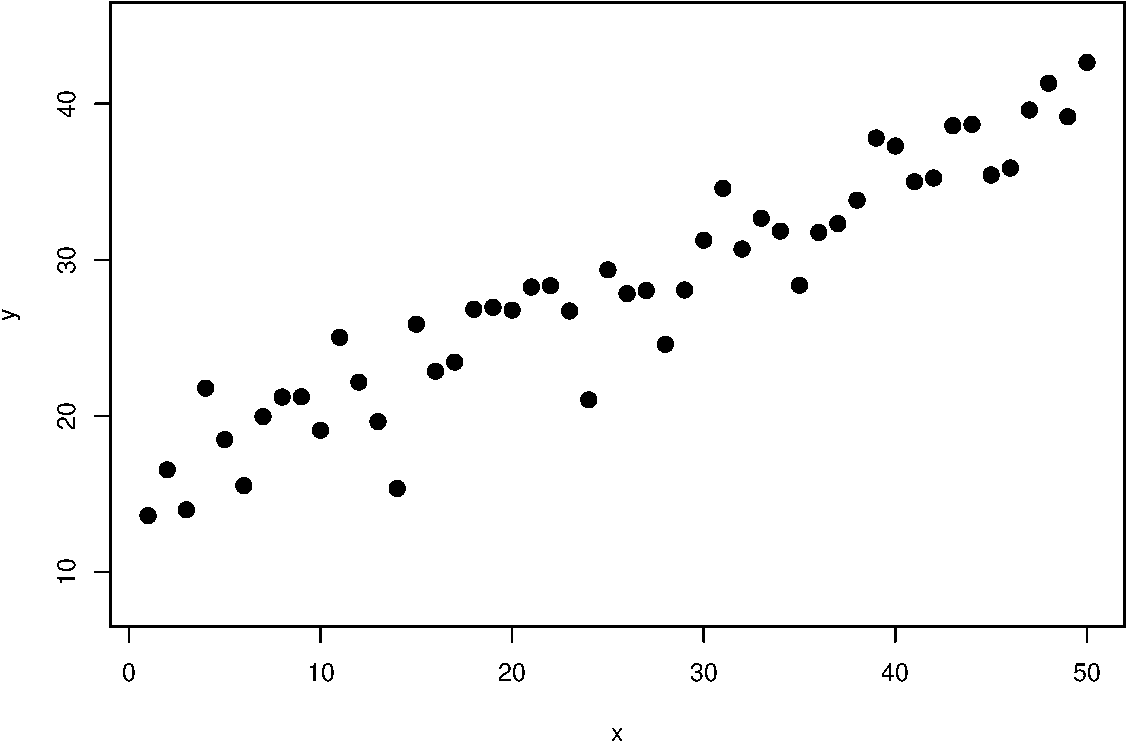
\includegraphics{index_files/figure-latex/unnamed-chunk-178-1.pdf}

A mathematical procedure for finding the best-fitting curve to a given
set of points by minimizing the sum of the squares of the residuals of
the points from the fitted line. Illustration of the least squares fit

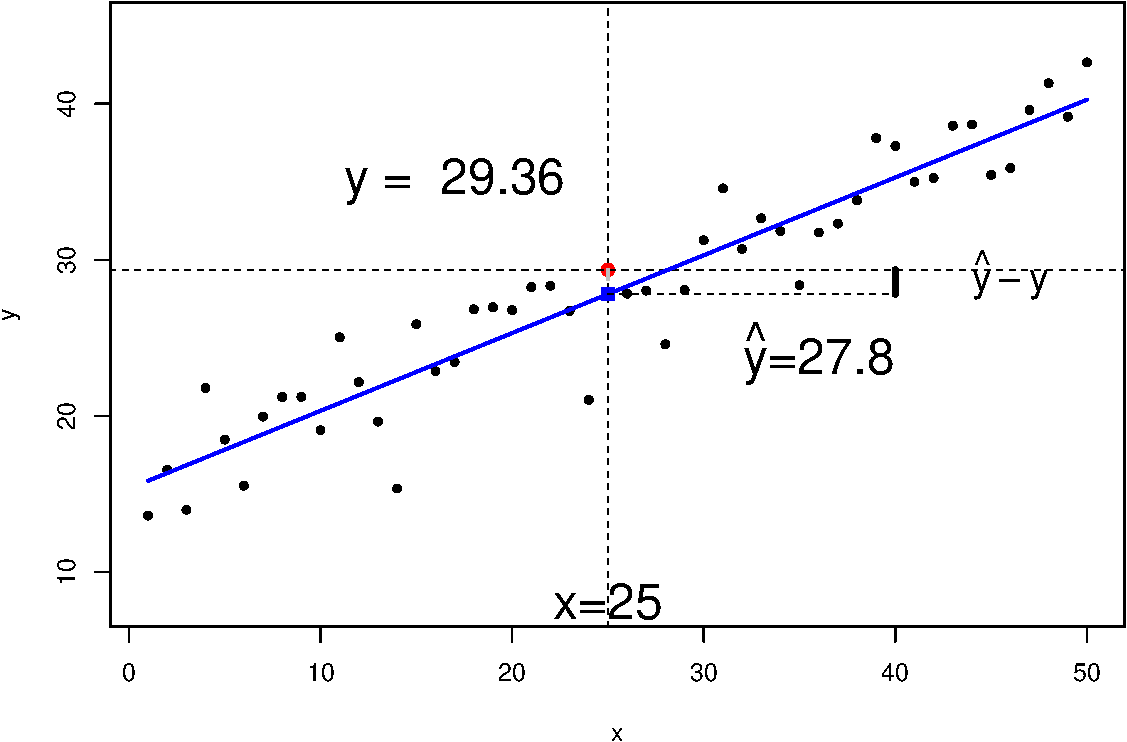
\includegraphics{index_files/figure-latex/unnamed-chunk-179-1.pdf}

For example, in the data set \texttt{faithful}, it contains sample data
of two random variables named \texttt{waiting} and \texttt{eruptions}.
The \texttt{waiting} variable denotes the waiting time until the next
eruptions, and \texttt{eruptions} denotes the duration.

\begin{Shaded}
\begin{Highlighting}[]
\KeywordTok{plot}\NormalTok{(eruptions~waiting,}\DataTypeTok{data=}\NormalTok{faithful)}
\end{Highlighting}
\end{Shaded}

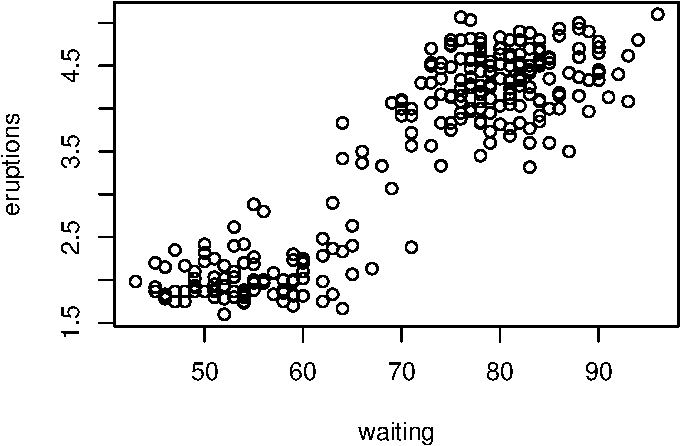
\includegraphics{index_files/figure-latex/unnamed-chunk-180-1.pdf}

Its linear regression model can be expressed as:

\[
Eruptions = \beta_0 + \beta_1*Waiting + \epsilon
\]

If we choose the parameters \(\beta_0\) and \(\beta_1\) in the simple
linear regression model so as to minimize the sum of squares of the
error term \(\epsilon\). Suppose for the data set \texttt{faithful}, we
aim to estimate the next eruption duration if the waiting time since the
last eruption has been 80 minutes.

We apply the \texttt{lm} function to a formula that describes the
variable eruptions by the variable waiting, and save the linear
regression model in a new variable \texttt{eruption.lm}.

\begin{Shaded}
\begin{Highlighting}[]
\KeywordTok{data}\NormalTok{(}\StringTok{"faithful"}\NormalTok{)}
\NormalTok{eruption.lm <-}\StringTok{ }\KeywordTok{lm}\NormalTok{(eruptions~waiting,}\DataTypeTok{data=}\NormalTok{faithful)}
\end{Highlighting}
\end{Shaded}

Then we extract the parameters of the estimated regression equation with
the coefficients function.

\begin{Shaded}
\begin{Highlighting}[]
\NormalTok{coeffs <-}\StringTok{ }\KeywordTok{coefficients}\NormalTok{(eruption.lm); coeffs }
\end{Highlighting}
\end{Shaded}

\begin{verbatim}
## (Intercept)     waiting 
## -1.87401599  0.07562795
\end{verbatim}

We now fit the eruption duration using the estimated regression
equation.

\begin{Shaded}
\begin{Highlighting}[]
\NormalTok{waiting =}\StringTok{ }\DecValTok{80}           \CommentTok{# the waiting time }
\NormalTok{duration =}\StringTok{ }\NormalTok{coeffs[}\DecValTok{1}\NormalTok{] +}\StringTok{ }\NormalTok{coeffs[}\DecValTok{2}\NormalTok{]*waiting }
\NormalTok{duration }
\end{Highlighting}
\end{Shaded}

\begin{verbatim}
## (Intercept) 
##     4.17622
\end{verbatim}

Based on the simple linear regression model, if the waiting time since
the last eruption has been 80 minutes, we expect the next one to last
4.1762198 minutes.

We wrap the waiting parameter value inside a new data frame named
newdata.

\begin{Shaded}
\begin{Highlighting}[]
\NormalTok{newdata =}\StringTok{ }\KeywordTok{data.frame}\NormalTok{(}\DataTypeTok{waiting=}\DecValTok{80}\NormalTok{) }\CommentTok{# wrap the parameter }
\end{Highlighting}
\end{Shaded}

Then we apply the \texttt{predict} function to \texttt{eruption.lm}
along with \texttt{newdata}.

\begin{Shaded}
\begin{Highlighting}[]
\KeywordTok{predict}\NormalTok{(eruption.lm, newdata)    }\CommentTok{# apply predict }
\end{Highlighting}
\end{Shaded}

\begin{verbatim}
##       1 
## 4.17622
\end{verbatim}

We can directly calculate quantities of interest, i.e.~the ordinary
least squares solution consists of:

\[
\min_{\beta_0,\beta_1} = \sum_{i=1}^{n} (y_i - \hat{y}_i)^2  
\]

Then \(\hat{\beta}_1 = \frac{\sum_{i=1}^{n}x_iy_i}{\sum_{i=1}^n x_i^2}\)
and \(\hat{\beta}_0 = \bar{y} - \hat{\beta}_1\bar{x}\)

In matrix form, with \(X=[1:x_1:...:x_p]\)

\[
\hat{\beta}  = (X^\prime X)^{-1} X^\prime
\]

where \(\hat{\beta} = (\hat{\beta}_0,\hat{\beta}_1)\)

\subsection{\texorpdfstring{Defining models in
\texttt{R}}{Defining models in R}}\label{defining-models-in-r}

To complete a linear regression using \texttt{R} it is first necessary
to understand the syntax for defining models.

\begin{longtable}[c]{@{}ccc@{}}
\toprule
\begin{minipage}[b]{0.27\columnwidth}\centering\strut
Syntax
\strut\end{minipage} &
\begin{minipage}[b]{0.55\columnwidth}\centering\strut
Model
\strut\end{minipage} &
\begin{minipage}[b]{0.90\columnwidth}\centering\strut
Comments
\strut\end{minipage}\tabularnewline
\midrule
\endhead
\begin{minipage}[t]{0.27\columnwidth}\centering\strut
\texttt{y\ \textasciitilde{}\ x}
\strut\end{minipage} &
\begin{minipage}[t]{0.55\columnwidth}\centering\strut
\(y = \beta_0+\beta_1x\)
\strut\end{minipage} &
\begin{minipage}[t]{0.90\columnwidth}\centering\strut
Straight-line with an implicit intercept
\strut\end{minipage}\tabularnewline
\begin{minipage}[t]{0.27\columnwidth}\centering\strut
\texttt{y\ \textasciitilde{}\ -1\ +\ x}
\strut\end{minipage} &
\begin{minipage}[t]{0.55\columnwidth}\centering\strut
\(y = \beta_1x\)
\strut\end{minipage} &
\begin{minipage}[t]{0.90\columnwidth}\centering\strut
Straight-line with no intercept; that is, a fit forced through (0,0)
\strut\end{minipage}\tabularnewline
\begin{minipage}[t]{0.27\columnwidth}\centering\strut
\texttt{y\ \textasciitilde{}\ x\ +\ I(x\^{}2)}
\strut\end{minipage} &
\begin{minipage}[t]{0.55\columnwidth}\centering\strut
\(y = \beta_0+\beta_1x+\beta_2x^2\)
\strut\end{minipage} &
\begin{minipage}[t]{0.90\columnwidth}\centering\strut
Polynomial model; \texttt{I()} allows for mathematical symbols
\strut\end{minipage}\tabularnewline
\begin{minipage}[t]{0.27\columnwidth}\centering\strut
\texttt{y\ \textasciitilde{}\ x\ +\ z}
\strut\end{minipage} &
\begin{minipage}[t]{0.55\columnwidth}\centering\strut
\(y = \beta_0+\beta_1x+\beta_2z\)
\strut\end{minipage} &
\begin{minipage}[t]{0.90\columnwidth}\centering\strut
Multiple regression model
\strut\end{minipage}\tabularnewline
\begin{minipage}[t]{0.27\columnwidth}\centering\strut
\texttt{y\ \textasciitilde{}\ x:z}
\strut\end{minipage} &
\begin{minipage}[t]{0.55\columnwidth}\centering\strut
\(y = \beta_0+\beta_1xz\)
\strut\end{minipage} &
\begin{minipage}[t]{0.90\columnwidth}\centering\strut
Model with interaction between \(x\) and \(z\)
\strut\end{minipage}\tabularnewline
\begin{minipage}[t]{0.27\columnwidth}\centering\strut
\texttt{y\ \textasciitilde{}\ x*z}
\strut\end{minipage} &
\begin{minipage}[t]{0.55\columnwidth}\centering\strut
\(y = \beta_0+\beta_1x+\beta_2z+\beta_3xz\)
\strut\end{minipage} &
\begin{minipage}[t]{0.90\columnwidth}\centering\strut
Equivalent to \texttt{y\textasciitilde{}x+z+x:z}
\strut\end{minipage}\tabularnewline
\bottomrule
\end{longtable}

In \texttt{R} function \texttt{model.matrix} helps us to create the
\(X\) matrix.

\begin{Shaded}
\begin{Highlighting}[]
\NormalTok{x <-}\StringTok{ }\KeywordTok{model.matrix}\NormalTok{(~waiting, }\DataTypeTok{data =} \NormalTok{faithful)}
\NormalTok{y <-}\StringTok{ }\NormalTok{faithful$eruptions}
\NormalTok{xtxi <-}\StringTok{ }\KeywordTok{solve}\NormalTok{(}\KeywordTok{t}\NormalTok{(x) %*%}\StringTok{ }\NormalTok{x)}
\NormalTok{betas <-}\StringTok{ }\NormalTok{xtxi %*%}\StringTok{ }\KeywordTok{t}\NormalTok{(x) %*%}\StringTok{ }\NormalTok{y}
\NormalTok{betas}
\end{Highlighting}
\end{Shaded}

\begin{verbatim}
##                    [,1]
## (Intercept) -1.87401599
## waiting      0.07562795
\end{verbatim}

or

\begin{Shaded}
\begin{Highlighting}[]
\KeywordTok{solve}\NormalTok{(}\KeywordTok{crossprod}\NormalTok{(x, x), }\KeywordTok{crossprod}\NormalTok{(x, y))}
\end{Highlighting}
\end{Shaded}

\begin{verbatim}
##                    [,1]
## (Intercept) -1.87401599
## waiting      0.07562795
\end{verbatim}

Of course, it is not necessary here because the \texttt{lm()} function
does the job but it is very useful when the statistic you want is not
part of the pre-packaged functions.

It is possible to get \((X^\prime X)^{-1}\) as

\begin{Shaded}
\begin{Highlighting}[]
\KeywordTok{summary}\NormalTok{(eruption.lm)$cov.unscaled}
\end{Highlighting}
\end{Shaded}

\begin{verbatim}
##              (Intercept)       waiting
## (Intercept)  0.104029479 -1.415475e-03
## waiting     -0.001415475  1.996521e-05
\end{verbatim}

The \texttt{names()} command is the way to see the components of an
\texttt{R} object

\begin{Shaded}
\begin{Highlighting}[]
\KeywordTok{names}\NormalTok{(eruption.lm)}
\end{Highlighting}
\end{Shaded}

\begin{verbatim}
##  [1] "coefficients"  "residuals"     "effects"       "rank"         
##  [5] "fitted.values" "assign"        "qr"            "df.residual"  
##  [9] "xlevels"       "call"          "terms"         "model"
\end{verbatim}

To access for example

\begin{itemize}
\tightlist
\item
  Fitted (or predictd) values (\(\hat{y}\)):
\end{itemize}

\begin{Shaded}
\begin{Highlighting}[]
\NormalTok{eruption.lm$fitted.values}
\end{Highlighting}
\end{Shaded}

\begin{itemize}
\tightlist
\item
  Residuals (\(y-\hat{y}\))
\end{itemize}

\begin{Shaded}
\begin{Highlighting}[]
\NormalTok{eruption.lm$residuals}
\end{Highlighting}
\end{Shaded}

We can estimate \(\sigma\) as \(\sigma = \frac{(y_i-\hat{y}_i)^2}{n-p}\)
in \texttt{R}

\begin{Shaded}
\begin{Highlighting}[]
\NormalTok{eruption.lm.sum <-}\StringTok{ }\KeywordTok{summary}\NormalTok{(eruption.lm)}
\KeywordTok{names}\NormalTok{(eruption.lm.sum)}
\end{Highlighting}
\end{Shaded}

\begin{verbatim}
##  [1] "call"          "terms"         "residuals"     "coefficients" 
##  [5] "aliased"       "sigma"         "df"            "r.squared"    
##  [9] "adj.r.squared" "fstatistic"    "cov.unscaled"
\end{verbatim}

\begin{Shaded}
\begin{Highlighting}[]
\KeywordTok{sqrt}\NormalTok{(}\KeywordTok{deviance}\NormalTok{(eruption.lm)/}\KeywordTok{df.residual}\NormalTok{(eruption.lm))}
\end{Highlighting}
\end{Shaded}

\begin{verbatim}
## [1] 0.4965129
\end{verbatim}

\begin{Shaded}
\begin{Highlighting}[]
\CommentTok{# is obtained directly as}
\NormalTok{eruption.lm.sum$sigma}
\end{Highlighting}
\end{Shaded}

\begin{verbatim}
## [1] 0.4965129
\end{verbatim}

We may also obtain the standard errors for the coefficients. Also
\texttt{diag()} returns the diagonal of a matrix:

\begin{Shaded}
\begin{Highlighting}[]
\NormalTok{xtxi }
\end{Highlighting}
\end{Shaded}

\begin{verbatim}
##              (Intercept)       waiting
## (Intercept)  0.104029479 -1.415475e-03
## waiting     -0.001415475  1.996521e-05
\end{verbatim}

\begin{Shaded}
\begin{Highlighting}[]
\KeywordTok{sqrt}\NormalTok{(}\KeywordTok{diag}\NormalTok{(xtxi)) *}\StringTok{ }\NormalTok{eruption.lm.sum$sigma}
\end{Highlighting}
\end{Shaded}

\begin{verbatim}
## (Intercept)     waiting 
## 0.160143302 0.002218541
\end{verbatim}

\begin{Shaded}
\begin{Highlighting}[]
\NormalTok{eruption.lm.sum$coef[, }\DecValTok{2}\NormalTok{]}
\end{Highlighting}
\end{Shaded}

\begin{verbatim}
## (Intercept)     waiting 
## 0.160143302 0.002218541
\end{verbatim}

\subsection{Coefficient of
Determination}\label{coefficient-of-determination}

The \textbf{coefficient of determination} of a linear regression model
is the quotient of the variances of the fitted values and observed
values of the dependent variable. If we denote \(y_i\) as the observed
values of the dependent variable, \(\bar{y}\) as its mean, and
\(\bar{y}_i\) as the fitted value, then the coefficient of determination
is: \[
    R^2 = \frac{\sum (\hat{y}_i-\bar{y})^2}{(y_i - \bar{y})^2}
\]

\begin{Shaded}
\begin{Highlighting}[]
\KeywordTok{summary}\NormalTok{(eruption.lm)$r.squared }
\end{Highlighting}
\end{Shaded}

\begin{verbatim}
## [1] 0.8114608
\end{verbatim}

or

\begin{Shaded}
\begin{Highlighting}[]
\DecValTok{1}\NormalTok{-}\KeywordTok{sum}\NormalTok{(eruption.lm$res^}\DecValTok{2}\NormalTok{)/}\KeywordTok{sum}\NormalTok{((y-}\KeywordTok{mean}\NormalTok{(y))^}\DecValTok{2}\NormalTok{)}
\end{Highlighting}
\end{Shaded}

\begin{verbatim}
## [1] 0.8114608
\end{verbatim}

More options:

\begin{itemize}
\item
  \texttt{fitted.values()} or \texttt{fitted()} Fitted values of the
  model
\item
  \texttt{predict()}: to predict \(\hat{y}_*\) for new values of \(x_*\)
\item
  \texttt{confint()}: confidence intervals for model parameters
\item
  \texttt{resid()}: residuals of the model
\item
  \texttt{anova()}: ANOVA table for residuals
\item
  \texttt{deviance()}: deviance of the fitted model, in the LM case is
  \(\sum_i^{n}(\hat{y}_i - y_i)^2\)
\end{itemize}

\emph{See Faraway's (2002) book (Chapters 1-7)}

\subsection{Significance Test for Linear
Regression}\label{significance-test-for-linear-regression}

Assume that the error term ?? in the linear regression model is
independent of x, and is normally distributed, with zero mean and
constant variance. We can decide whether there is any significant
relationship between x and y by testing the null hypothesis that
\(\beta_1 = 0\).

we print out the F-statistics of the significance test with the summary
function.

\begin{Shaded}
\begin{Highlighting}[]
\KeywordTok{summary}\NormalTok{(eruption.lm) }
\end{Highlighting}
\end{Shaded}

\begin{verbatim}
## 
## Call:
## lm(formula = eruptions ~ waiting, data = faithful)
## 
## Residuals:
##      Min       1Q   Median       3Q      Max 
## -1.29917 -0.37689  0.03508  0.34909  1.19329 
## 
## Coefficients:
##              Estimate Std. Error t value Pr(>|t|)    
## (Intercept) -1.874016   0.160143  -11.70   <2e-16 ***
## waiting      0.075628   0.002219   34.09   <2e-16 ***
## ---
## Signif. codes:  0 '***' 0.001 '**' 0.01 '*' 0.05 '.' 0.1 ' ' 1
## 
## Residual standard error: 0.4965 on 270 degrees of freedom
## Multiple R-squared:  0.8115, Adjusted R-squared:  0.8108 
## F-statistic:  1162 on 1 and 270 DF,  p-value: < 2.2e-16
\end{verbatim}

\subsection{Confidence Interval for Linear
Regression}\label{confidence-interval-for-linear-regression}

Assume that the error term \(\epsilon\) in the linear regression model
is independent of \(x\), and is normally distributed, with zero mean and
constant variance. For a given value of \(x\), the interval estimate for
the mean of the dependent variable, \(\bar{y}\) , is called the
confidence interval.

A 95\% confidence interval of the mean eruption duration for the waiting
time of 80 minutes is given by

\begin{Shaded}
\begin{Highlighting}[]
\KeywordTok{predict}\NormalTok{(eruption.lm, newdata, }\DataTypeTok{interval=}\StringTok{"confidence"}\NormalTok{) }
\end{Highlighting}
\end{Shaded}

\begin{verbatim}
##       fit      lwr      upr
## 1 4.17622 4.104848 4.247592
\end{verbatim}

The 95\% confidence interval of the mean eruption duration for the
waiting time of 80 minutes is between 4.1048 and 4.2476 minutes.

\subsection{Prediction Interval for Linear
Regression}\label{prediction-interval-for-linear-regression}

For a given value of \(x\), the interval estimate of the dependent
variable \(y\) is called the prediction interval.

\begin{Shaded}
\begin{Highlighting}[]
\KeywordTok{predict}\NormalTok{(eruption.lm, newdata, }\DataTypeTok{interval=}\StringTok{"predict"}\NormalTok{) }
\end{Highlighting}
\end{Shaded}

\begin{verbatim}
##       fit      lwr      upr
## 1 4.17622 3.196089 5.156351
\end{verbatim}

The 95\% prediction interval of the eruption duration for the waiting
time of 80 minutes is between 3.1961 and 5.1564 minutes.

\subsection{Residual Plot}\label{residual-plot}

The residual data of the simple linear regression model is the
difference between the observed data of the dependent variable \(y\) and
the fitted values \(\hat{y}\).

\[
    Residual = y -\hat{y}
\]

\begin{Shaded}
\begin{Highlighting}[]
\NormalTok{eruption.res =}\StringTok{ }\KeywordTok{resid}\NormalTok{(eruption.lm) }
\end{Highlighting}
\end{Shaded}

\begin{Shaded}
\begin{Highlighting}[]
\KeywordTok{plot}\NormalTok{(faithful$waiting,}
    \NormalTok{eruption.res, }
    \DataTypeTok{ylab=}\StringTok{"Residuals"}\NormalTok{, }\DataTypeTok{xlab=}\StringTok{"Waiting Time"}\NormalTok{, }
    \DataTypeTok{main=}\StringTok{"Old Faithful Eruptions"}\NormalTok{) }
\KeywordTok{abline}\NormalTok{(}\DecValTok{0}\NormalTok{, }\DecValTok{0}\NormalTok{)}
\end{Highlighting}
\end{Shaded}

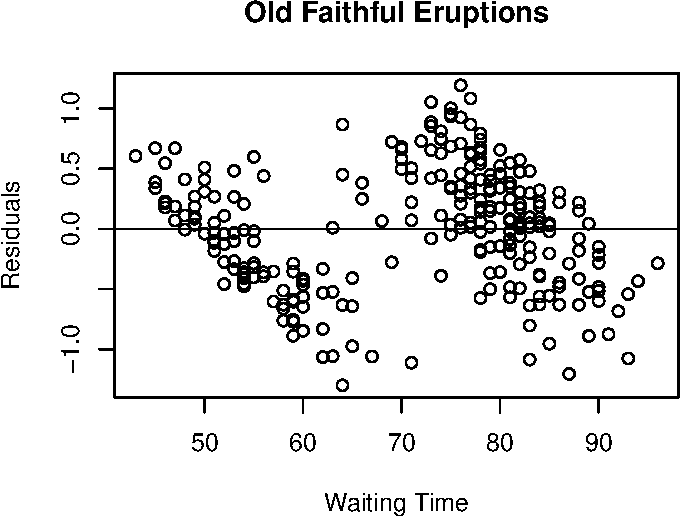
\includegraphics{index_files/figure-latex/unnamed-chunk-200-1.pdf}

\subsection{Standardized Residual}\label{standardized-residual}

The standardized residual is the residual divided by its standard
deviation.

\[
\mbox{Standardized residual}_i =  \frac{Residual_i}{SD.of.Residual_i}
\]

\begin{Shaded}
\begin{Highlighting}[]
\NormalTok{eruption.stdres <-}\StringTok{ }\KeywordTok{rstandard}\NormalTok{(eruption.lm) }
\end{Highlighting}
\end{Shaded}

\begin{Shaded}
\begin{Highlighting}[]
\KeywordTok{plot}\NormalTok{(faithful$waiting, eruption.stdres, }
      \DataTypeTok{ylab=}\StringTok{"Standardized Residuals"}\NormalTok{, }
      \DataTypeTok{xlab=}\StringTok{"Waiting Time"}\NormalTok{, }
      \DataTypeTok{main=}\StringTok{"Old Faithful Eruptions"}\NormalTok{) }
\KeywordTok{abline}\NormalTok{(}\DecValTok{0}\NormalTok{, }\DecValTok{0}\NormalTok{)}
\end{Highlighting}
\end{Shaded}

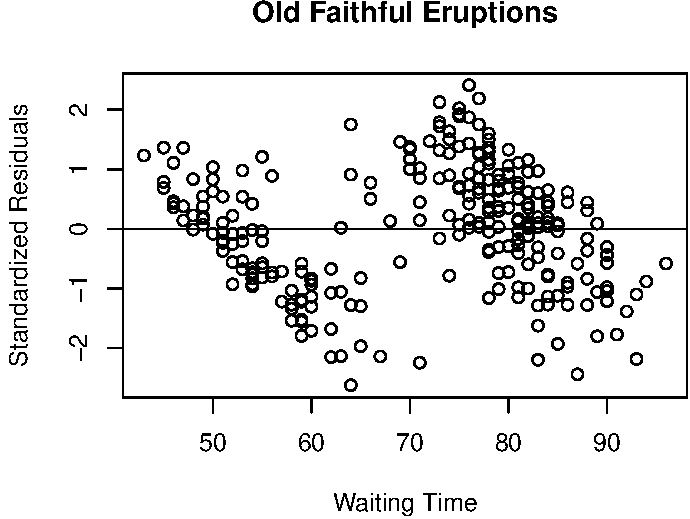
\includegraphics{index_files/figure-latex/unnamed-chunk-202-1.pdf}

As the p-value is much less than \(0.05\), we reject the null hypothesis
that \(\beta_1 = 0\). Hence there is a significant relationship between
the variables in the linear regression model of the data set faithful.

\subsection{Normal Probability Plot of
Residuals}\label{normal-probability-plot-of-residuals}

The normal probability plot is a graphical tool for comparing a data set
with the normal distribution. We can use it with the standardized
residual of the linear regression model and see if the error term
\(\epsilon\) is actually normally distributed.

\begin{Shaded}
\begin{Highlighting}[]
\NormalTok{eruption.lm =}\StringTok{ }\KeywordTok{lm}\NormalTok{(eruptions ~}\StringTok{ }\NormalTok{waiting, }\DataTypeTok{data=}\NormalTok{faithful) }
\NormalTok{eruption.stdres =}\StringTok{ }\KeywordTok{rstandard}\NormalTok{(eruption.lm) }
\end{Highlighting}
\end{Shaded}

We now create the normal probability plot with the \texttt{qqnorm}
function, and add the \texttt{qqline} for further comparison.

\begin{Shaded}
\begin{Highlighting}[]
 \KeywordTok{qqnorm}\NormalTok{(eruption.stdres, }
     \DataTypeTok{ylab=}\StringTok{"Standardized Residuals"}\NormalTok{, }
     \DataTypeTok{xlab=}\StringTok{"Normal Scores"}\NormalTok{, }
     \DataTypeTok{main=}\StringTok{"Old Faithful Eruptions"}\NormalTok{) }
 \KeywordTok{qqline}\NormalTok{(eruption.stdres) }
\end{Highlighting}
\end{Shaded}

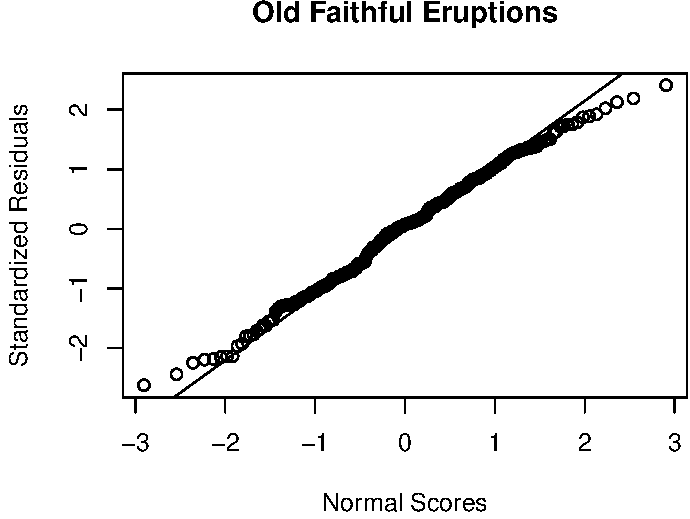
\includegraphics{index_files/figure-latex/unnamed-chunk-204-1.pdf}

\subsection{Multiple linear
regression}\label{multiple-linear-regression}

A multiple linear regression (MLR) model that describes a dependent
variable \(y\) by independent variables \(x_1, x_2, ..., x_p\)
\((p > 1)\) is expressed by the equation: \[
    y  = \beta_0 + \sum_{k}^{p} \beta_k + \epsilon
\] where the numbers \(\beta_0\) and \(\beta_k\) (\(k = 1, 2, ..., p\))
are the parameters, and \(\epsilon\) is the error term.

\textbf{Example:}

Consider the data \texttt{stackloss} from observations of a chemical
plant operation, if we assign \texttt{stackloss} as the dependent
variable, and assign \texttt{Air.Flow} (cooling air flow),
\texttt{Water.Temp} (inlet water temperature) and \texttt{Acid.Conc.}
(acid concentration) as independent variables, the multiple linear
regression model is:

\[
      stack.loss = \beta_0 + \beta_1 * Air.Flow + \beta_2 * Water.Temp + \beta_3 * Acid.Conc + \epsilon
\]

\begin{Shaded}
\begin{Highlighting}[]
\KeywordTok{data}\NormalTok{(}\StringTok{"stackloss"}\NormalTok{)}
\NormalTok{?stackloss}
\KeywordTok{head}\NormalTok{(stackloss)}
\end{Highlighting}
\end{Shaded}

\begin{verbatim}
##   Air.Flow Water.Temp Acid.Conc. stack.loss
## 1       80         27         89         42
## 2       80         27         88         37
## 3       75         25         90         37
## 4       62         24         87         28
## 5       62         22         87         18
## 6       62         23         87         18
\end{verbatim}

Fit the multiple linear regression in \texttt{R}

\begin{Shaded}
\begin{Highlighting}[]
\NormalTok{stackloss.lm =}\StringTok{ }\KeywordTok{lm}\NormalTok{(stack.loss ~}\StringTok{ }\NormalTok{Air.Flow +}\StringTok{ }\NormalTok{Water.Temp +}\StringTok{ }\NormalTok{Acid.Conc., }\DataTypeTok{data=}\NormalTok{stackloss) }
\NormalTok{stackloss.lm}
\end{Highlighting}
\end{Shaded}

\begin{verbatim}
## 
## Call:
## lm(formula = stack.loss ~ Air.Flow + Water.Temp + Acid.Conc., 
##     data = stackloss)
## 
## Coefficients:
## (Intercept)     Air.Flow   Water.Temp   Acid.Conc.  
##    -39.9197       0.7156       1.2953      -0.1521
\end{verbatim}

\begin{Shaded}
\begin{Highlighting}[]
\KeywordTok{summary}\NormalTok{(stackloss.lm)}
\end{Highlighting}
\end{Shaded}

\begin{verbatim}
## 
## Call:
## lm(formula = stack.loss ~ Air.Flow + Water.Temp + Acid.Conc., 
##     data = stackloss)
## 
## Residuals:
##     Min      1Q  Median      3Q     Max 
## -7.2377 -1.7117 -0.4551  2.3614  5.6978 
## 
## Coefficients:
##             Estimate Std. Error t value Pr(>|t|)    
## (Intercept) -39.9197    11.8960  -3.356  0.00375 ** 
## Air.Flow      0.7156     0.1349   5.307  5.8e-05 ***
## Water.Temp    1.2953     0.3680   3.520  0.00263 ** 
## Acid.Conc.   -0.1521     0.1563  -0.973  0.34405    
## ---
## Signif. codes:  0 '***' 0.001 '**' 0.01 '*' 0.05 '.' 0.1 ' ' 1
## 
## Residual standard error: 3.243 on 17 degrees of freedom
## Multiple R-squared:  0.9136, Adjusted R-squared:  0.8983 
## F-statistic:  59.9 on 3 and 17 DF,  p-value: 3.016e-09
\end{verbatim}

Function \texttt{termplot} plots regression terms against their
predictors:

\begin{Shaded}
\begin{Highlighting}[]
\NormalTok{?termplot}
\KeywordTok{par}\NormalTok{(}\DataTypeTok{mfrow=}\KeywordTok{c}\NormalTok{(}\DecValTok{2}\NormalTok{,}\DecValTok{2}\NormalTok{))}
\KeywordTok{termplot}\NormalTok{(stackloss.lm, }\DataTypeTok{partial.resid =} \OtherTok{TRUE}\NormalTok{, }\DataTypeTok{se=}\OtherTok{TRUE}\NormalTok{,}\DataTypeTok{col.se =} \StringTok{"blue"}\NormalTok{)}
\end{Highlighting}
\end{Shaded}

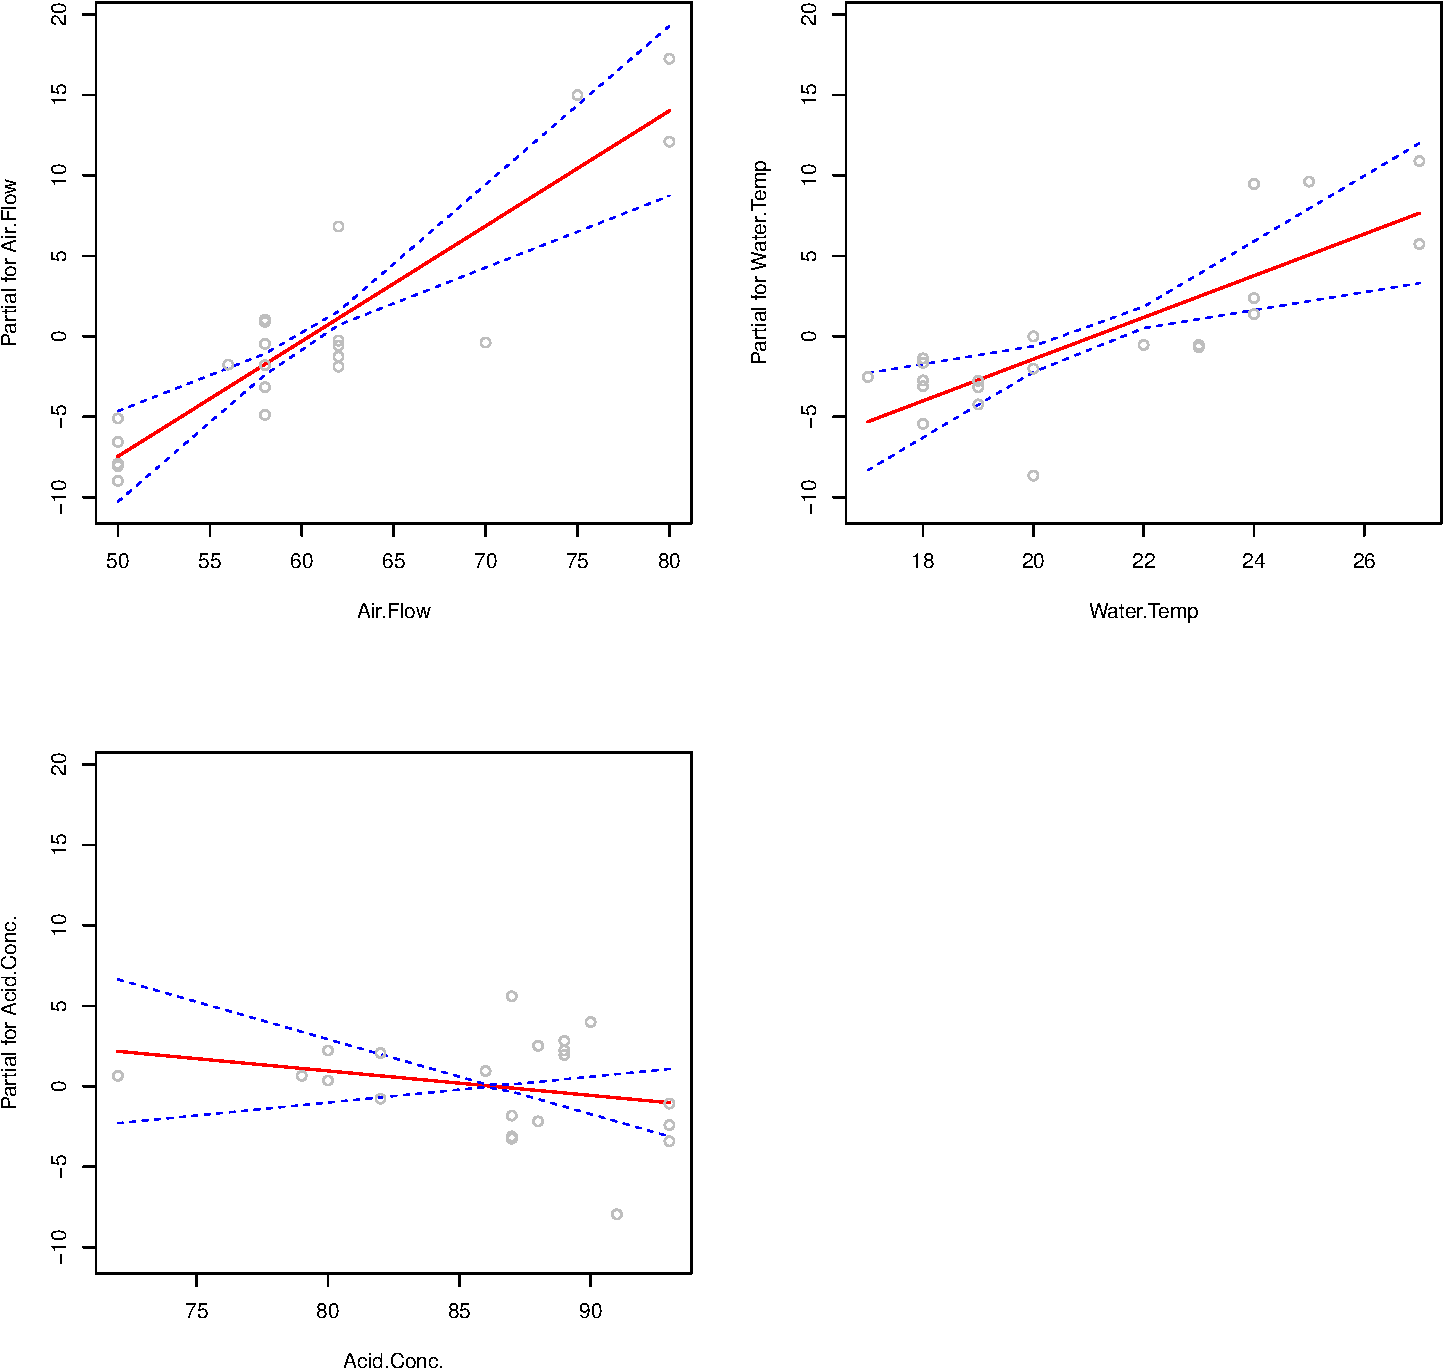
\includegraphics{index_files/figure-latex/unnamed-chunk-207-1.pdf}

\textbf{What is the stack loss if the air flow is 72, water temperature
is 20 and acid concentration is 85?}

Create a new data frame:

\begin{Shaded}
\begin{Highlighting}[]
\NormalTok{newdata <-}\StringTok{ }\KeywordTok{data.frame}\NormalTok{(}\DataTypeTok{Air.Flow=}\DecValTok{72}\NormalTok{,}\DataTypeTok{Water.Temp=}\DecValTok{20}\NormalTok{,}\DataTypeTok{Acid.Conc.=}\DecValTok{85}\NormalTok{)}
\end{Highlighting}
\end{Shaded}

Use \texttt{predict}

\begin{Shaded}
\begin{Highlighting}[]
\KeywordTok{predict}\NormalTok{(stackloss.lm, newdata) }
\end{Highlighting}
\end{Shaded}

\begin{verbatim}
##        1 
## 24.58173
\end{verbatim}

Based on the multiple linear regression model and the given parameters,
the predicted stack loss is 24.5817284.

To obtain the multiple coefficient of determination

\begin{Shaded}
\begin{Highlighting}[]
\KeywordTok{summary}\NormalTok{(stackloss.lm)$r.squared }
\end{Highlighting}
\end{Shaded}

\begin{verbatim}
## [1] 0.9135769
\end{verbatim}

\subsubsection{Adjusted coefficient of
determination}\label{adjusted-coefficient-of-determination}

The adjusted coefficient of determination of a multiple linear
regression model is defined in terms of the coefficient of determination
as follows, where \(n\) is the number of observations in the data set,
and \(p\) is the number of independent variables.

\[
R^2_{adj} = 1-(1-R^2)\frac{n-1}{n-p-1}
\]

\begin{Shaded}
\begin{Highlighting}[]
\KeywordTok{summary}\NormalTok{(stackloss.lm)$adj.r.squared }
\end{Highlighting}
\end{Shaded}

\begin{verbatim}
## [1] 0.8983258
\end{verbatim}

\subsubsection{Significant tests and confidence/prediction
intervals}\label{significant-tests-and-confidenceprediction-intervals}

\begin{Shaded}
\begin{Highlighting}[]
\KeywordTok{summary}\NormalTok{(stackloss.lm)}
\end{Highlighting}
\end{Shaded}

\begin{verbatim}
## 
## Call:
## lm(formula = stack.loss ~ Air.Flow + Water.Temp + Acid.Conc., 
##     data = stackloss)
## 
## Residuals:
##     Min      1Q  Median      3Q     Max 
## -7.2377 -1.7117 -0.4551  2.3614  5.6978 
## 
## Coefficients:
##             Estimate Std. Error t value Pr(>|t|)    
## (Intercept) -39.9197    11.8960  -3.356  0.00375 ** 
## Air.Flow      0.7156     0.1349   5.307  5.8e-05 ***
## Water.Temp    1.2953     0.3680   3.520  0.00263 ** 
## Acid.Conc.   -0.1521     0.1563  -0.973  0.34405    
## ---
## Signif. codes:  0 '***' 0.001 '**' 0.01 '*' 0.05 '.' 0.1 ' ' 1
## 
## Residual standard error: 3.243 on 17 degrees of freedom
## Multiple R-squared:  0.9136, Adjusted R-squared:  0.8983 
## F-statistic:  59.9 on 3 and 17 DF,  p-value: 3.016e-09
\end{verbatim}

As the p-values of \texttt{Air.Flow} and \texttt{Water.Temp} are less
than 0.05, they are both statistically significant in the multiple
linear regression model of \texttt{stackloss}.

95\% Confidence intervals of the stack loss if the air flow is 72, water
temperature is 20 and acid concentration is 85.

\begin{Shaded}
\begin{Highlighting}[]
\KeywordTok{predict}\NormalTok{(stackloss.lm, newdata, }\DataTypeTok{interval=}\StringTok{"confidence"}\NormalTok{)}
\end{Highlighting}
\end{Shaded}

\begin{verbatim}
##        fit      lwr    upr
## 1 24.58173 20.21846 28.945
\end{verbatim}

95\% Prediction intervals are

\begin{Shaded}
\begin{Highlighting}[]
\KeywordTok{predict}\NormalTok{(stackloss.lm, newdata, }\DataTypeTok{interval=}\StringTok{"prediction"}\NormalTok{)}
\end{Highlighting}
\end{Shaded}

\begin{verbatim}
##        fit     lwr      upr
## 1 24.58173 16.4661 32.69736
\end{verbatim}

\subsection{Linear regression with factor
variables}\label{linear-regression-with-factor-variables}

Let us consider the \texttt{mtcars} we analyzed previously. In
\protect\hyperlink{population-mean-between-two-independent-samples}{Section}.

\begin{Shaded}
\begin{Highlighting}[]
\KeywordTok{data}\NormalTok{(mtcars)}
\KeywordTok{t.test}\NormalTok{(mpg ~}\StringTok{ }\NormalTok{am, }\DataTypeTok{data=}\NormalTok{mtcars) }
\end{Highlighting}
\end{Shaded}

\begin{verbatim}
## 
##  Welch Two Sample t-test
## 
## data:  mpg by am
## t = -3.7671, df = 18.332, p-value = 0.001374
## alternative hypothesis: true difference in means is not equal to 0
## 95 percent confidence interval:
##  -11.280194  -3.209684
## sample estimates:
## mean in group 0 mean in group 1 
##        17.14737        24.39231
\end{verbatim}

The results from the statistical tests focus on \texttt{mpg} and
\texttt{am} only, without controlling for influences from other
variables.

The benefit of regressional analysis serve the purpose. If we apply a
multivariate regression to control for certain available design and
performance variables, the marginal impact of automatic- or manual-
transmission cars does not turn out to be significant. The confounding
variables include displacement (disp), rear axle ratio (drat) and car
weight(wt). Take car weight for example. The regression suggests that,
holding other variables constant (ceteris paribus), maual tramsmitted
cars consume on avarage -0.024 more gallons of gas per mile, and the
results are no longer statistically significant. Similar analysis work
similarily for the other two variables: drat and wt.

\begin{Shaded}
\begin{Highlighting}[]
\NormalTok{fit0 <-}\StringTok{ }\KeywordTok{lm}\NormalTok{(mpg ~}\StringTok{ }\KeywordTok{factor}\NormalTok{(am), }\DataTypeTok{data =} \NormalTok{mtcars)}
\KeywordTok{summary}\NormalTok{(fit0)}
\end{Highlighting}
\end{Shaded}

\begin{verbatim}
## 
## Call:
## lm(formula = mpg ~ factor(am), data = mtcars)
## 
## Residuals:
##     Min      1Q  Median      3Q     Max 
## -9.3923 -3.0923 -0.2974  3.2439  9.5077 
## 
## Coefficients:
##             Estimate Std. Error t value Pr(>|t|)    
## (Intercept)   17.147      1.125  15.247 1.13e-15 ***
## factor(am)1    7.245      1.764   4.106 0.000285 ***
## ---
## Signif. codes:  0 '***' 0.001 '**' 0.01 '*' 0.05 '.' 0.1 ' ' 1
## 
## Residual standard error: 4.902 on 30 degrees of freedom
## Multiple R-squared:  0.3598, Adjusted R-squared:  0.3385 
## F-statistic: 16.86 on 1 and 30 DF,  p-value: 0.000285
\end{verbatim}

If we apply a multivariate regression to control for certain available
design and performance variables, the marginal impact of automatic- or
manual- transmission cars does not turn out to be significant. The
confounding variables include displacement (\texttt{disp}), rear axle
ratio (\texttt{drat}) and car weight(\texttt{wt}). Take car weight for
example:

\begin{Shaded}
\begin{Highlighting}[]
\NormalTok{fit1 <-}\StringTok{ }\KeywordTok{lm}\NormalTok{(mpg ~}\StringTok{ }\KeywordTok{factor}\NormalTok{(am) +}\StringTok{ }\NormalTok{wt, }\DataTypeTok{data =} \NormalTok{mtcars)}
\KeywordTok{summary}\NormalTok{(fit1)}
\end{Highlighting}
\end{Shaded}

\begin{verbatim}
## 
## Call:
## lm(formula = mpg ~ factor(am) + wt, data = mtcars)
## 
## Residuals:
##     Min      1Q  Median      3Q     Max 
## -4.5295 -2.3619 -0.1317  1.4025  6.8782 
## 
## Coefficients:
##             Estimate Std. Error t value Pr(>|t|)    
## (Intercept) 37.32155    3.05464  12.218 5.84e-13 ***
## factor(am)1 -0.02362    1.54565  -0.015    0.988    
## wt          -5.35281    0.78824  -6.791 1.87e-07 ***
## ---
## Signif. codes:  0 '***' 0.001 '**' 0.01 '*' 0.05 '.' 0.1 ' ' 1
## 
## Residual standard error: 3.098 on 29 degrees of freedom
## Multiple R-squared:  0.7528, Adjusted R-squared:  0.7358 
## F-statistic: 44.17 on 2 and 29 DF,  p-value: 1.579e-09
\end{verbatim}

The regression suggests that, holding other variables constant, manual
tramsmitted cars consume on average -0.024 more gallons of gas per mile,
and the results are no longer statistically significant. Similar
analysis work similarily for the other two variables: \texttt{drat} and
\texttt{wt}.

\begin{Shaded}
\begin{Highlighting}[]
\NormalTok{fit2 <-}\StringTok{ }\KeywordTok{lm}\NormalTok{(mpg ~}\StringTok{ }\KeywordTok{factor}\NormalTok{(am) +}\StringTok{ }\NormalTok{drat, }\DataTypeTok{data =} \NormalTok{mtcars)}
\KeywordTok{summary}\NormalTok{(fit2)}
\end{Highlighting}
\end{Shaded}

\begin{verbatim}
## 
## Call:
## lm(formula = mpg ~ factor(am) + drat, data = mtcars)
## 
## Residuals:
##     Min      1Q  Median      3Q     Max 
## -9.5802 -2.5206 -0.5153  2.4419  8.5198 
## 
## Coefficients:
##             Estimate Std. Error t value Pr(>|t|)  
## (Intercept)   -1.950      7.073  -0.276   0.7848  
## factor(am)1    2.807      2.282   1.230   0.2286  
## drat           5.811      2.130   2.728   0.0107 *
## ---
## Signif. codes:  0 '***' 0.001 '**' 0.01 '*' 0.05 '.' 0.1 ' ' 1
## 
## Residual standard error: 4.448 on 29 degrees of freedom
## Multiple R-squared:  0.4906, Adjusted R-squared:  0.4554 
## F-statistic: 13.96 on 2 and 29 DF,  p-value: 5.659e-05
\end{verbatim}

\begin{Shaded}
\begin{Highlighting}[]
\NormalTok{fit3 <-}\StringTok{ }\KeywordTok{lm}\NormalTok{(mpg ~}\StringTok{ }\KeywordTok{factor}\NormalTok{(am) +}\StringTok{ }\NormalTok{disp, }\DataTypeTok{data =} \NormalTok{mtcars)}
\KeywordTok{summary}\NormalTok{(fit3)}
\end{Highlighting}
\end{Shaded}

\begin{verbatim}
## 
## Call:
## lm(formula = mpg ~ factor(am) + disp, data = mtcars)
## 
## Residuals:
##     Min      1Q  Median      3Q     Max 
## -4.6382 -2.4751 -0.5631  2.2333  6.8386 
## 
## Coefficients:
##              Estimate Std. Error t value Pr(>|t|)    
## (Intercept) 27.848081   1.834071  15.184 2.45e-15 ***
## factor(am)1  1.833458   1.436100   1.277    0.212    
## disp        -0.036851   0.005782  -6.373 5.75e-07 ***
## ---
## Signif. codes:  0 '***' 0.001 '**' 0.01 '*' 0.05 '.' 0.1 ' ' 1
## 
## Residual standard error: 3.218 on 29 degrees of freedom
## Multiple R-squared:  0.7333, Adjusted R-squared:  0.7149 
## F-statistic: 39.87 on 2 and 29 DF,  p-value: 4.749e-09
\end{verbatim}

We can use \texttt{termplot}

\begin{Shaded}
\begin{Highlighting}[]
\KeywordTok{termplot}\NormalTok{(fit0,}\DataTypeTok{partial.resid =} \OtherTok{TRUE}\NormalTok{,}\DataTypeTok{se=}\OtherTok{TRUE}\NormalTok{)}
\end{Highlighting}
\end{Shaded}

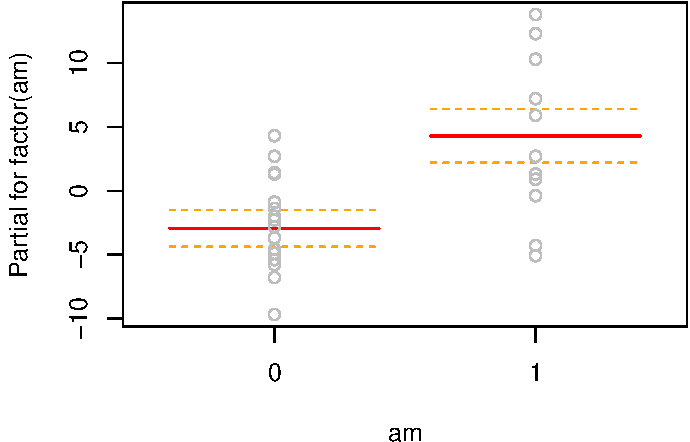
\includegraphics{index_files/figure-latex/unnamed-chunk-219-1.pdf}

\begin{Shaded}
\begin{Highlighting}[]
\KeywordTok{par}\NormalTok{(}\DataTypeTok{mfrow=}\KeywordTok{c}\NormalTok{(}\DecValTok{1}\NormalTok{,}\DecValTok{2}\NormalTok{))}
\KeywordTok{termplot}\NormalTok{(fit1,}\DataTypeTok{partial.resid =} \OtherTok{TRUE}\NormalTok{,}\DataTypeTok{se=}\OtherTok{TRUE}\NormalTok{)}
\end{Highlighting}
\end{Shaded}

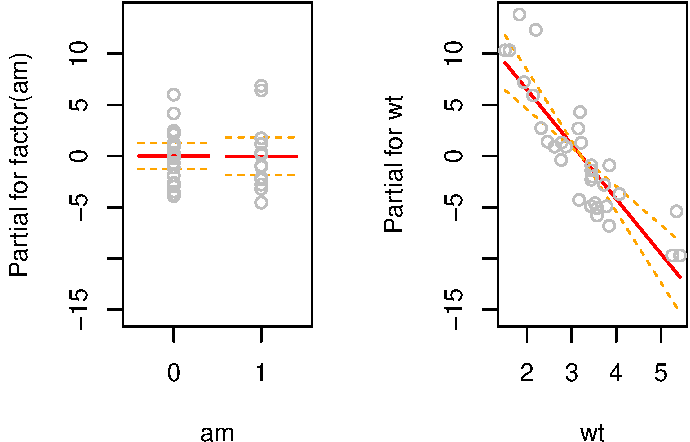
\includegraphics{index_files/figure-latex/unnamed-chunk-220-1.pdf}

\begin{Shaded}
\begin{Highlighting}[]
\KeywordTok{termplot}\NormalTok{(fit2,}\DataTypeTok{partial.resid =} \OtherTok{TRUE}\NormalTok{,}\DataTypeTok{se=}\OtherTok{TRUE}\NormalTok{)}
\end{Highlighting}
\end{Shaded}

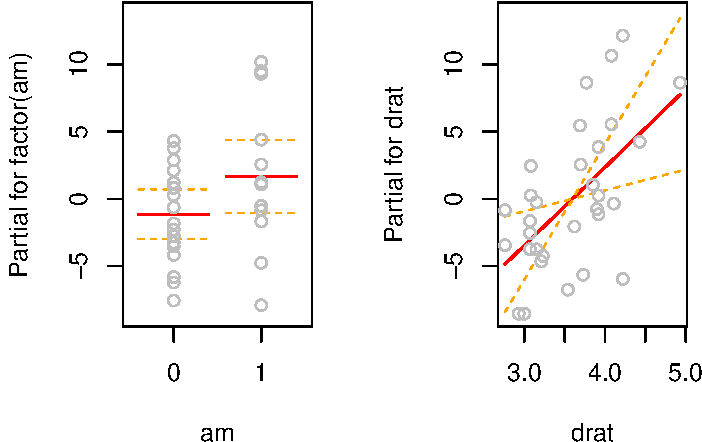
\includegraphics{index_files/figure-latex/unnamed-chunk-220-2.pdf}

\subsection{Inference}\label{inference}

\textbf{Hypothesis test to compare models: the Likelihood ratio test}

A likelihood ratio test is a statistical test used to compare the
goodness of fit of two models, one of which (the null model) is a
special case of the other (the alternative model). The test is based on
the likelihood ratio, which expresses how many times more likely the
data are under one model than the other.

Comparing two models fit to the same data can be set up as a hypothesis
testing problem. Let \(M_0\) and \(M_1\) denote the models. Consider as
the null hypothesis ``\(M_1\) is not a significant improvement on
\(M_0\)'', and the alternative the negation. This hypothesis can often
be formulated so that a statistic can be generated from the two models.

Normally, the models are nested in that the variables in \(M_0\) are a
subset of those in \(M_1\). The statistic often involves the \(RSS\)
(residual sum of squares) values for both models, adjusted by the number
of parameters used. In linear regression this becomes an \texttt{anova}
test (comparing variances).

More robust is a likelihood ratio test for nested models. When models
are sufficiently specific to define a probability distribution for
\(y\), the model will report the log-likelihood, \(\hat{L}\). Under some
mild assumptions, \(-2(\hat{L}_0 - \hat{L}_1)\) follows a Chi-squared
distribution with degrees of freedom = difference in number of
parameters on the two models.

The utility of a single model \(M_1\) is often assessed by comparing it
with the null model, that reflects no dependence of \(y\) on the
explanatory variables. The model formula for the null model is
\texttt{y\textasciitilde{}1}, i.e.~we use a constant to approximate
\texttt{y} (e.g.: the mean of \texttt{y}). The likelihood ratio test is
implemented in the function \texttt{anova}:

\begin{Shaded}
\begin{Highlighting}[]
\NormalTok{M0 <-}\StringTok{ }\KeywordTok{lm}\NormalTok{(mpg ~}\StringTok{ }\DecValTok{1}\NormalTok{, }\DataTypeTok{data =} \NormalTok{mtcars)}
\NormalTok{M1 <-}\StringTok{ }\KeywordTok{lm}\NormalTok{(mpg ~}\StringTok{ }\KeywordTok{factor}\NormalTok{(am), }\DataTypeTok{data =} \NormalTok{mtcars)}
\KeywordTok{summary}\NormalTok{(M0)}
\end{Highlighting}
\end{Shaded}

\begin{verbatim}
## 
## Call:
## lm(formula = mpg ~ 1, data = mtcars)
## 
## Residuals:
##     Min      1Q  Median      3Q     Max 
## -9.6906 -4.6656 -0.8906  2.7094 13.8094 
## 
## Coefficients:
##             Estimate Std. Error t value Pr(>|t|)    
## (Intercept)   20.091      1.065   18.86   <2e-16 ***
## ---
## Signif. codes:  0 '***' 0.001 '**' 0.01 '*' 0.05 '.' 0.1 ' ' 1
## 
## Residual standard error: 6.027 on 31 degrees of freedom
\end{verbatim}

\begin{Shaded}
\begin{Highlighting}[]
\KeywordTok{summary}\NormalTok{(M1)}
\end{Highlighting}
\end{Shaded}

\begin{verbatim}
## 
## Call:
## lm(formula = mpg ~ factor(am), data = mtcars)
## 
## Residuals:
##     Min      1Q  Median      3Q     Max 
## -9.3923 -3.0923 -0.2974  3.2439  9.5077 
## 
## Coefficients:
##             Estimate Std. Error t value Pr(>|t|)    
## (Intercept)   17.147      1.125  15.247 1.13e-15 ***
## factor(am)1    7.245      1.764   4.106 0.000285 ***
## ---
## Signif. codes:  0 '***' 0.001 '**' 0.01 '*' 0.05 '.' 0.1 ' ' 1
## 
## Residual standard error: 4.902 on 30 degrees of freedom
## Multiple R-squared:  0.3598, Adjusted R-squared:  0.3385 
## F-statistic: 16.86 on 1 and 30 DF,  p-value: 0.000285
\end{verbatim}

\begin{Shaded}
\begin{Highlighting}[]
\KeywordTok{anova}\NormalTok{(M0,M1)}
\end{Highlighting}
\end{Shaded}

\begin{verbatim}
## Analysis of Variance Table
## 
## Model 1: mpg ~ 1
## Model 2: mpg ~ factor(am)
##   Res.Df    RSS Df Sum of Sq     F   Pr(>F)    
## 1     31 1126.0                                
## 2     30  720.9  1    405.15 16.86 0.000285 ***
## ---
## Signif. codes:  0 '***' 0.001 '**' 0.01 '*' 0.05 '.' 0.1 ' ' 1
\end{verbatim}

The likelihood ratio test can also test the significance of predictors.
Hence, we can compare the model \texttt{fit0} (where \texttt{am} is
significant) with \texttt{fit1}, \texttt{fit2} or \texttt{fit3}, i.e.:

\begin{Shaded}
\begin{Highlighting}[]
\KeywordTok{anova}\NormalTok{(fit0, fit1)}
\end{Highlighting}
\end{Shaded}

\begin{verbatim}
## Analysis of Variance Table
## 
## Model 1: mpg ~ factor(am)
## Model 2: mpg ~ factor(am) + wt
##   Res.Df    RSS Df Sum of Sq      F    Pr(>F)    
## 1     30 720.90                                  
## 2     29 278.32  1    442.58 46.115 1.867e-07 ***
## ---
## Signif. codes:  0 '***' 0.001 '**' 0.01 '*' 0.05 '.' 0.1 ' ' 1
\end{verbatim}

\begin{Shaded}
\begin{Highlighting}[]
\KeywordTok{anova}\NormalTok{(fit0, fit2)}
\end{Highlighting}
\end{Shaded}

\begin{verbatim}
## Analysis of Variance Table
## 
## Model 1: mpg ~ factor(am)
## Model 2: mpg ~ factor(am) + drat
##   Res.Df    RSS Df Sum of Sq      F Pr(>F)  
## 1     30 720.90                             
## 2     29 573.64  1    147.26 7.4444 0.0107 *
## ---
## Signif. codes:  0 '***' 0.001 '**' 0.01 '*' 0.05 '.' 0.1 ' ' 1
\end{verbatim}

\begin{Shaded}
\begin{Highlighting}[]
\KeywordTok{anova}\NormalTok{(fit0, fit3)}
\end{Highlighting}
\end{Shaded}

\begin{verbatim}
## Analysis of Variance Table
## 
## Model 1: mpg ~ factor(am)
## Model 2: mpg ~ factor(am) + disp
##   Res.Df    RSS Df Sum of Sq      F    Pr(>F)    
## 1     30 720.90                                  
## 2     29 300.28  1    420.62 40.621 5.748e-07 ***
## ---
## Signif. codes:  0 '***' 0.001 '**' 0.01 '*' 0.05 '.' 0.1 ' ' 1
\end{verbatim}

However, the likelihood ratio tests suggest that it is important to
consider these dimensions (i.e., displacement, rear axle ratio and
weight) since these variables increase model fit.

\subsection{ANALYSIS-OF-VARIANCE
(ANOVA)}\label{analysis-of-variance-anova}

In an experiment study, various treatments are applied to test subjects
and the response data is gathered for analysis. A critical tool for
carrying out the analysis is the Analysis of Variance (ANOVA). It
enables a researcher to differentiate treatment results based on easily
computed statistical quantities from the treatment outcome.

The statistical process is derived from estimates of the population
variances via two separate approaches. The first approach is based on
the variance of the sample means, and the second one is based on the
mean of the sample variances. Under the ANOVA assumptions as stated
below, the ratio of the two statistical estimates follows the F
distribution. Hence we can test the null hypothesis on the equality of
various response data from different treatments via estimates of
critical regions.

\begin{verbatim}
The treatment responses are independent of each other.
The response data follow the normal distribution.
The variances of the response data are identical.
\end{verbatim}

In the following tutorials, we demonstrate how to perform ANOVA on a few
basic experimental designs.

\begin{Shaded}
\begin{Highlighting}[]
\CommentTok{# Two-way Interaction Plot}
\KeywordTok{data}\NormalTok{(mtcars)}
\KeywordTok{attach}\NormalTok{(mtcars)}
\end{Highlighting}
\end{Shaded}

\begin{verbatim}
## The following objects are masked from mtcars (pos = 11):
## 
##     am, carb, cyl, disp, drat, gear, hp, mpg, qsec, vs, wt
\end{verbatim}

\begin{Shaded}
\begin{Highlighting}[]
\NormalTok{gear <-}\StringTok{ }\KeywordTok{factor}\NormalTok{(gear)}
\NormalTok{cyl <-}\StringTok{ }\KeywordTok{factor}\NormalTok{(cyl)}
\KeywordTok{interaction.plot}\NormalTok{(cyl, gear, mpg, }\DataTypeTok{type=}\StringTok{"b"}\NormalTok{, }\DataTypeTok{col=}\KeywordTok{c}\NormalTok{(}\DecValTok{1}\NormalTok{:}\DecValTok{3}\NormalTok{),}
   \DataTypeTok{leg.bty=}\StringTok{"o"}\NormalTok{, }\DataTypeTok{leg.bg=}\StringTok{"beige"}\NormalTok{, }\DataTypeTok{lwd=}\DecValTok{2}\NormalTok{, }\DataTypeTok{pch=}\KeywordTok{c}\NormalTok{(}\DecValTok{18}\NormalTok{,}\DecValTok{24}\NormalTok{,}\DecValTok{22}\NormalTok{),}
   \DataTypeTok{xlab=}\StringTok{"Number of Cylinders"}\NormalTok{,}
   \DataTypeTok{ylab=}\StringTok{"Mean Miles Per Gallon"}\NormalTok{,}
   \DataTypeTok{main=}\StringTok{"Interaction Plot"}\NormalTok{)}
\end{Highlighting}
\end{Shaded}

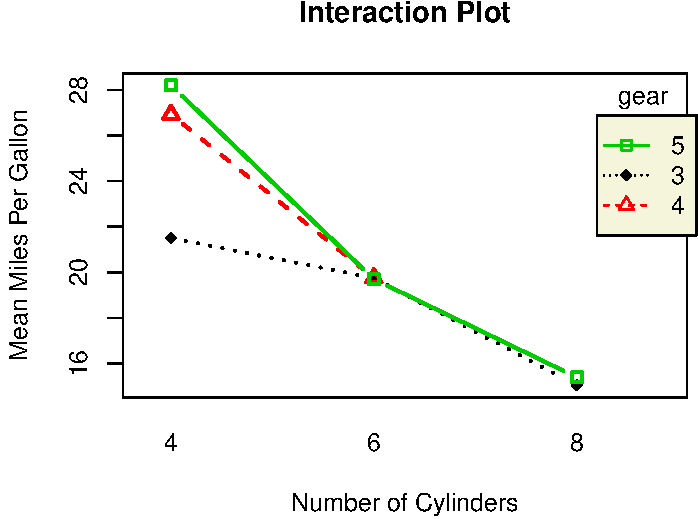
\includegraphics{index_files/figure-latex/unnamed-chunk-223-1.pdf}

\begin{Shaded}
\begin{Highlighting}[]
\CommentTok{# Plot Means with Error Bars}
\KeywordTok{library}\NormalTok{(gplots)}
\KeywordTok{attach}\NormalTok{(mtcars)}
\end{Highlighting}
\end{Shaded}

\begin{verbatim}
## The following objects are masked _by_ .GlobalEnv:
## 
##     cyl, gear
\end{verbatim}

\begin{verbatim}
## The following objects are masked from mtcars (pos = 3):
## 
##     am, carb, cyl, disp, drat, gear, hp, mpg, qsec, vs, wt
\end{verbatim}

\begin{verbatim}
## The following objects are masked from mtcars (pos = 12):
## 
##     am, carb, cyl, disp, drat, gear, hp, mpg, qsec, vs, wt
\end{verbatim}

\begin{Shaded}
\begin{Highlighting}[]
\NormalTok{cyl <-}\StringTok{ }\KeywordTok{factor}\NormalTok{(cyl)}
\KeywordTok{plotmeans}\NormalTok{(mpg~cyl,}\DataTypeTok{xlab=}\StringTok{"Number of Cylinders"}\NormalTok{,}
  \DataTypeTok{ylab=}\StringTok{"Miles Per Gallon"}\NormalTok{, }\DataTypeTok{main=}\StringTok{"Mean Plot}\CharTok{\textbackslash{}n}\StringTok{with 95% CI"}\NormalTok{) }
\end{Highlighting}
\end{Shaded}

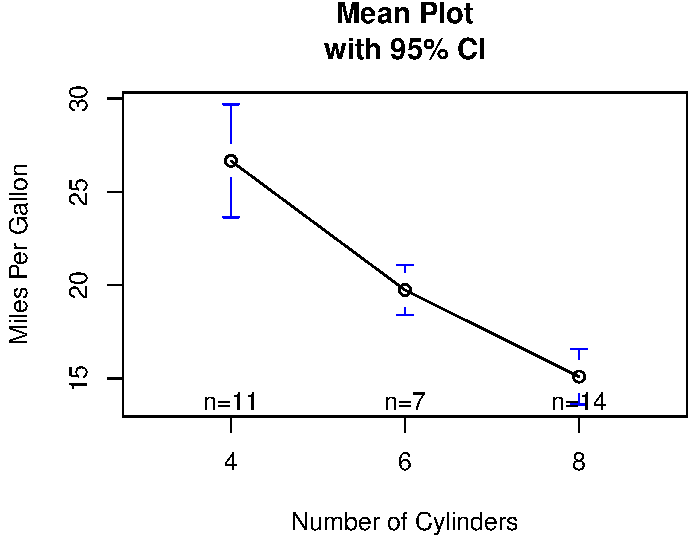
\includegraphics{index_files/figure-latex/unnamed-chunk-224-1.pdf}

\section{Logistic regression}\label{logistic-regression}

A logistic regression is typically used when there is one dichotomous
outcome variable (such as winning or losing), and a continuous predictor
variable which is related to the probability or odds of the outcome
variable. It can also be used with categorical predictors, and with
multiple predictors.

\subsection{ESR and Plasma Proteins}\label{esr-and-plasma-proteins}

The erythrocyte sedimentation rate (ESR) is the rate at which red blood
cells (erythrocytes) settle out of suspension in blood plasma, when
measured under standard conditions. If the ESR increases when the level
of certain proteins in the blood plasma rise in association with
conditions such as rheumatic diseases, chronic infections and malignant
diseases, its determination might be useful in screening blood samples
taken from people suspected of suffering from one of the conditions
mentioned. The absolute value of the ESR is not of great importance;
rather, less than 20mm/hr indicates a ``healthy'' individual. To assess
whether the ESR is a useful diagnostic tool, the question of interest is
whether there is any association between the probability of an ESR
reading greater than 20mm/hr and the levels of the two plasma proteins.
If there is not then the determination of ESR would not be useful for
diagnostic purposes. A data frame with 32 observations on the following
3 variables.

\begin{itemize}
\tightlist
\item
  \texttt{fibrinogen} the fibrinogen level in the blood.
\item
  \texttt{globulin} the globulin level in the blood.
\item
  \texttt{ESR} the erythrocyte sedimentation rate, either less or
  greater 20 mm / hour.
\end{itemize}

\begin{Shaded}
\begin{Highlighting}[]
\KeywordTok{data}\NormalTok{(}\StringTok{"plasma"}\NormalTok{, }\DataTypeTok{package =} \StringTok{"HSAUR"}\NormalTok{)}
\KeywordTok{head}\NormalTok{(plasma)}
\end{Highlighting}
\end{Shaded}

\begin{verbatim}
##   fibrinogen globulin      ESR
## 1       2.52       38 ESR < 20
## 2       2.56       31 ESR < 20
## 3       2.19       33 ESR < 20
## 4       2.18       31 ESR < 20
## 5       3.41       37 ESR < 20
## 6       2.46       36 ESR < 20
\end{verbatim}

\begin{Shaded}
\begin{Highlighting}[]
\KeywordTok{layout}\NormalTok{(}\KeywordTok{matrix}\NormalTok{(}\DecValTok{1}\NormalTok{:}\DecValTok{2}\NormalTok{, }\DataTypeTok{ncol =} \DecValTok{2}\NormalTok{))}
\KeywordTok{boxplot}\NormalTok{(fibrinogen ~}\StringTok{ }\NormalTok{ESR, }\DataTypeTok{data =} \NormalTok{plasma, }\DataTypeTok{varwidth =} \OtherTok{TRUE}\NormalTok{, }\DataTypeTok{main=}\StringTok{"Fibrinogen level in the blood"}\NormalTok{)}
\KeywordTok{boxplot}\NormalTok{(globulin ~}\StringTok{ }\NormalTok{ESR, }\DataTypeTok{data =} \NormalTok{plasma, }\DataTypeTok{varwidth =} \OtherTok{TRUE}\NormalTok{, }\DataTypeTok{main=}\StringTok{"Globulin level in the blood"}\NormalTok{)}
\end{Highlighting}
\end{Shaded}

\includegraphics{index_files/figure-latex/unnamed-chunk-226-1.pdf}

The question of interest is whether there is any association between the
probability of an ESR reading greater than 20mm/hr and the levels of the
two plasma proteins. If there is not then the determination of ESR would
not be useful for diagnostic purposes.

Since the response variable is binary, a multiple regression model is
not suitable for a regression analysis.

We may write \[
\mathbb{P}\mbox{r}(y_i=1)=\pi_i \qquad \mathbb{P}\mbox{r}(y_i=0)=1-\pi_i
\]

Normally, we will have a set of covariates \(X=(x_1,..., x_p)\)
associated with each individual, and our goal will be to investigate the
relationship between the response probability \(\pi=\pi(X)\) and the
explanatory variables.

So instead of modelling the expected value of the response directly as a
linear function of explanatory variables, a suitable transformation is
modelled. In this case the most suitable transformation is the logistic
or logit function of \(\pi\) leading to the model

\[
  \mbox{logit}(\pi) = \mbox{logit}\left(\frac{\pi}{1-\pi}\right) = \beta_0 + \beta_1x_1 + ... + \beta_p x_p
\]

The logit of a probability is simply the log of the odds of the response
taking the value one or logit transformation, of p:
\(logit(p) = \log(p/1-p)\). Logit is sometimes called ``log odds.''
Because of the properties of odds given in the list above, the logit has
these properties:

\begin{itemize}
\tightlist
\item
  If \texttt{odds(y=1s)\ =\ 1}, then \texttt{logit(p)\ =\ 0}.
\item
  If \texttt{odds(y=1)\ \textless{}\ 1}, then
  \texttt{logit(p)\ \textless{}\ 0}.
\item
  If \texttt{odds(y=1)\ \textgreater{}\ 1}, then
  \texttt{logit(p)\ \textgreater{}\ 0}.
\end{itemize}

The logit transform fails if p = 0`.

When the response is a binary (dichotomous) variable, and x is numeric,
logistic regression fits a logistic curve to the relationship between
\(x\) and \(y\). Hence, logistic regression is linear regression on the
logit transform of y, where y is the proportion (or probability) of
success at each value of x. However, you should avoid the temptation to
do a traditional least-squares regression at this point, as neither the
normality nor the homoscedasticity assumption will be met.

\begin{Shaded}
\begin{Highlighting}[]
\NormalTok{x <-}\StringTok{ }\KeywordTok{seq}\NormalTok{(-}\DecValTok{6}\NormalTok{,}\DecValTok{6}\NormalTok{,}\FloatTok{0.01}\NormalTok{)}
\NormalTok{logistic <-}\StringTok{ }\KeywordTok{exp}\NormalTok{(x)/(}\DecValTok{1}\NormalTok{+}\KeywordTok{exp}\NormalTok{(x))}
\KeywordTok{plot}\NormalTok{(x,logistic,}\DataTypeTok{t=}\StringTok{'l'}\NormalTok{,}\DataTypeTok{main=}\StringTok{"Logistic curve"}\NormalTok{,}\DataTypeTok{ylab=}\StringTok{""}\NormalTok{)}
\KeywordTok{abline}\NormalTok{(}\DataTypeTok{h=}\KeywordTok{c}\NormalTok{(}\DecValTok{0}\NormalTok{,}\FloatTok{0.5}\NormalTok{,}\DecValTok{1}\NormalTok{),}\DataTypeTok{v=}\DecValTok{0}\NormalTok{,}\DataTypeTok{col=}\StringTok{"grey"}\NormalTok{)}
\KeywordTok{points}\NormalTok{(}\DecValTok{0}\NormalTok{,}\FloatTok{0.5}\NormalTok{,}\DataTypeTok{pch=}\DecValTok{19}\NormalTok{,}\DataTypeTok{col=}\DecValTok{2}\NormalTok{)}
\end{Highlighting}
\end{Shaded}

\includegraphics{index_files/figure-latex/unnamed-chunk-227-1.pdf}

Logistic regression model in \texttt{R} can be fitted using the function
\texttt{glm}. First, we start with a model that includes only a single
predictor \texttt{fibrinogen}

\begin{Shaded}
\begin{Highlighting}[]
\NormalTok{plasma_glm_1 <-}\StringTok{ }\KeywordTok{glm}\NormalTok{(ESR ~}\StringTok{ }\NormalTok{fibrinogen, }\DataTypeTok{data =} \NormalTok{plasma,}\DataTypeTok{family =} \KeywordTok{binomial}\NormalTok{())}
\KeywordTok{summary}\NormalTok{(plasma_glm_1)}
\end{Highlighting}
\end{Shaded}

\begin{verbatim}
## 
## Call:
## glm(formula = ESR ~ fibrinogen, family = binomial(), data = plasma)
## 
## Deviance Residuals: 
##     Min       1Q   Median       3Q      Max  
## -0.9298  -0.5399  -0.4382  -0.3356   2.4794  
## 
## Coefficients:
##             Estimate Std. Error z value Pr(>|z|)  
## (Intercept)  -6.8451     2.7703  -2.471   0.0135 *
## fibrinogen    1.8271     0.9009   2.028   0.0425 *
## ---
## Signif. codes:  0 '***' 0.001 '**' 0.01 '*' 0.05 '.' 0.1 ' ' 1
## 
## (Dispersion parameter for binomial family taken to be 1)
## 
##     Null deviance: 30.885  on 31  degrees of freedom
## Residual deviance: 24.840  on 30  degrees of freedom
## AIC: 28.84
## 
## Number of Fisher Scoring iterations: 5
\end{verbatim}

We see that the regression coefficient for \texttt{fibrinogen} is
significant at the \(5\%\) level. An increase of one unit in this
variable increases the log-odds in favour of an ESR value greater than
20 by an estimated \(1.83\) with \(95\%\) confidence interval.

\begin{Shaded}
\begin{Highlighting}[]
\KeywordTok{confint}\NormalTok{(plasma_glm_1,}\DataTypeTok{parm=}\StringTok{"fibrinogen"}\NormalTok{)}
\end{Highlighting}
\end{Shaded}

\begin{verbatim}
## Waiting for profiling to be done...
\end{verbatim}

\begin{verbatim}
##     2.5 %    97.5 % 
## 0.3387619 3.9984921
\end{verbatim}

These values are more helpful if converted to the corresponding values
for the odds themselves by exponentiating the estimate

\begin{Shaded}
\begin{Highlighting}[]
\KeywordTok{exp}\NormalTok{(}\KeywordTok{coef}\NormalTok{(plasma_glm_1)[}\StringTok{"fibrinogen"}\NormalTok{])}
\end{Highlighting}
\end{Shaded}

\begin{verbatim}
## fibrinogen 
##   6.215715
\end{verbatim}

and the confidence interval

\begin{Shaded}
\begin{Highlighting}[]
\KeywordTok{exp}\NormalTok{(}\KeywordTok{confint}\NormalTok{(plasma_glm_1, }\DataTypeTok{parm =} \StringTok{"fibrinogen"}\NormalTok{))}
\end{Highlighting}
\end{Shaded}

\begin{verbatim}
## Waiting for profiling to be done...
\end{verbatim}

\begin{verbatim}
##     2.5 %    97.5 % 
##  1.403209 54.515884
\end{verbatim}

The confidence interval is very wide because there are few observations
overall and very few where the ESR value is greater than 20.
Nevertheless it seems likely that increased values of fibrinogen lead to
a greater probability of an ESR value greater than 20. We can now fit a
logistic regression model that includes both explanatory variables using
the code

\begin{Shaded}
\begin{Highlighting}[]
\NormalTok{plasma_glm_2 <-}\StringTok{ }\KeywordTok{glm}\NormalTok{(ESR ~}\StringTok{ }\NormalTok{fibrinogen +}\StringTok{ }\NormalTok{globulin, }\DataTypeTok{data =} \NormalTok{plasma,}\DataTypeTok{family =} \KeywordTok{binomial}\NormalTok{())}
\KeywordTok{summary}\NormalTok{(plasma_glm_2)}
\end{Highlighting}
\end{Shaded}

\begin{verbatim}
## 
## Call:
## glm(formula = ESR ~ fibrinogen + globulin, family = binomial(), 
##     data = plasma)
## 
## Deviance Residuals: 
##     Min       1Q   Median       3Q      Max  
## -0.9683  -0.6122  -0.3458  -0.2116   2.2636  
## 
## Coefficients:
##             Estimate Std. Error z value Pr(>|z|)  
## (Intercept) -12.7921     5.7963  -2.207   0.0273 *
## fibrinogen    1.9104     0.9710   1.967   0.0491 *
## globulin      0.1558     0.1195   1.303   0.1925  
## ---
## Signif. codes:  0 '***' 0.001 '**' 0.01 '*' 0.05 '.' 0.1 ' ' 1
## 
## (Dispersion parameter for binomial family taken to be 1)
## 
##     Null deviance: 30.885  on 31  degrees of freedom
## Residual deviance: 22.971  on 29  degrees of freedom
## AIC: 28.971
## 
## Number of Fisher Scoring iterations: 5
\end{verbatim}

The coefficient for gamma globulin is not significantly different from
zero.

Both nested models can be compared using a likelihood ratio test with
\texttt{anova} function

\begin{Shaded}
\begin{Highlighting}[]
\KeywordTok{anova}\NormalTok{(plasma_glm_1, plasma_glm_2, }\DataTypeTok{test =} \StringTok{"Chisq"}\NormalTok{)}
\end{Highlighting}
\end{Shaded}

\begin{verbatim}
## Analysis of Deviance Table
## 
## Model 1: ESR ~ fibrinogen
## Model 2: ESR ~ fibrinogen + globulin
##   Resid. Df Resid. Dev Df Deviance Pr(>Chi)
## 1        30     24.840                     
## 2        29     22.971  1   1.8692   0.1716
\end{verbatim}

So we conclude that gamma globulin is not associated with ESR level.

The plot clearly shows the increasing probability of an ESR value above
20 (larger circles) as the values of fibrinogen, and to a lesser extent,
gamma globulin, increase.

\begin{Shaded}
\begin{Highlighting}[]
\NormalTok{prob <-}\StringTok{ }\KeywordTok{predict}\NormalTok{(plasma_glm_2,}\DataTypeTok{type=}\StringTok{"response"}\NormalTok{)}
\KeywordTok{plot}\NormalTok{(globulin ~}\StringTok{ }\NormalTok{fibrinogen, }\DataTypeTok{data =} \NormalTok{plasma, }\DataTypeTok{xlim =} \KeywordTok{c}\NormalTok{(}\DecValTok{2}\NormalTok{, }\DecValTok{6}\NormalTok{),}\DataTypeTok{ylim =} \KeywordTok{c}\NormalTok{(}\DecValTok{25}\NormalTok{, }\DecValTok{55}\NormalTok{), }\DataTypeTok{pch =} \StringTok{"."}\NormalTok{)}
\KeywordTok{symbols}\NormalTok{(plasma$fibrinogen, plasma$globulin, }\DataTypeTok{circles =} \NormalTok{prob,}\DataTypeTok{add =} \OtherTok{TRUE}\NormalTok{)}
\end{Highlighting}
\end{Shaded}

\includegraphics{index_files/figure-latex/unnamed-chunk-234-1.pdf}

\section{\texorpdfstring{Advanced graphics in
\texttt{R}}{Advanced graphics in R}}\label{advanced-graphics-in-r}

\subsection{\texorpdfstring{\texttt{lattice}}{lattice}}\label{lattice}

\subsection{\texorpdfstring{\texttt{ggplot2}}{ggplot2}}\label{ggplot2}

Why \texttt{ggplot2}?

Advantages of \texttt{ggplot2}

\begin{itemize}
\tightlist
\item
  consistent underlying grammar of graphics (Wilkinson, 2005)
\item
  plot specification at a high level of abstraction
\item
  very flexible
\item
  theme system for polishing plot appearance
\item
  mature and complete graphics system
\item
  many users, active mailing list
\end{itemize}

\begin{Shaded}
\begin{Highlighting}[]
\KeywordTok{library}\NormalTok{(ggplot2)}
\NormalTok{?qplot}
\KeywordTok{qplot}\NormalTok{(displ, hwy, }\DataTypeTok{data =} \NormalTok{mpg, }\DataTypeTok{colour =} \KeywordTok{factor}\NormalTok{(cyl))}
\end{Highlighting}
\end{Shaded}

\includegraphics{index_files/figure-latex/unnamed-chunk-235-1.pdf}

\begin{Shaded}
\begin{Highlighting}[]
\KeywordTok{qplot}\NormalTok{(mpg, wt, }\DataTypeTok{data =} \NormalTok{mtcars)}
\end{Highlighting}
\end{Shaded}

\includegraphics{index_files/figure-latex/unnamed-chunk-235-2.pdf}

\begin{Shaded}
\begin{Highlighting}[]
\KeywordTok{qplot}\NormalTok{(mpg, wt, }\DataTypeTok{data =} \NormalTok{mtcars, }\DataTypeTok{colour =} \NormalTok{cyl)}
\end{Highlighting}
\end{Shaded}

\includegraphics{index_files/figure-latex/unnamed-chunk-235-3.pdf}

\begin{Shaded}
\begin{Highlighting}[]
\KeywordTok{qplot}\NormalTok{(mpg, wt, }\DataTypeTok{data =} \NormalTok{mtcars, }\DataTypeTok{size =} \NormalTok{cyl)}
\end{Highlighting}
\end{Shaded}

\includegraphics{index_files/figure-latex/unnamed-chunk-235-4.pdf}

\begin{Shaded}
\begin{Highlighting}[]
\KeywordTok{qplot}\NormalTok{(mpg, wt, }\DataTypeTok{data =} \NormalTok{mtcars, }\DataTypeTok{size =} \NormalTok{cyl, }\DataTypeTok{alpha =} \KeywordTok{I}\NormalTok{(}\FloatTok{0.7}\NormalTok{))}
\end{Highlighting}
\end{Shaded}

\includegraphics{index_files/figure-latex/unnamed-chunk-235-5.pdf}

\begin{Shaded}
\begin{Highlighting}[]
\KeywordTok{qplot}\NormalTok{(mpg, wt, }\DataTypeTok{data =} \NormalTok{mtcars, }\DataTypeTok{facets =} \NormalTok{vs ~}\StringTok{ }\NormalTok{am)}
\end{Highlighting}
\end{Shaded}

\includegraphics{index_files/figure-latex/unnamed-chunk-235-6.pdf}

\begin{Shaded}
\begin{Highlighting}[]
\KeywordTok{qplot}\NormalTok{(displ, hwy, }\DataTypeTok{data=}\NormalTok{mpg, }\DataTypeTok{facets =} \NormalTok{. ~}\StringTok{ }\NormalTok{year) +}\StringTok{ }\KeywordTok{geom_smooth}\NormalTok{()}
\end{Highlighting}
\end{Shaded}

\includegraphics{index_files/figure-latex/unnamed-chunk-235-7.pdf}

\begin{Shaded}
\begin{Highlighting}[]
\NormalTok{p <-}\StringTok{ }\KeywordTok{ggplot}\NormalTok{(mtcars)}
\NormalTok{p <-}\StringTok{ }\NormalTok{p +}\StringTok{ }\KeywordTok{aes}\NormalTok{(wt, hp)}
\NormalTok{p}
\end{Highlighting}
\end{Shaded}

\includegraphics{index_files/figure-latex/unnamed-chunk-235-8.pdf}

\begin{Shaded}
\begin{Highlighting}[]
\NormalTok{p +}\StringTok{ }\KeywordTok{geom_point}\NormalTok{(}\KeywordTok{aes}\NormalTok{(}\DataTypeTok{colour =} \KeywordTok{factor}\NormalTok{(cyl)))}
\end{Highlighting}
\end{Shaded}

\includegraphics{index_files/figure-latex/unnamed-chunk-235-9.pdf}

\begin{Shaded}
\begin{Highlighting}[]
\NormalTok{p +}\StringTok{ }\KeywordTok{geom_point}\NormalTok{(}\KeywordTok{aes}\NormalTok{(}\DataTypeTok{y =} \NormalTok{disp))}
\end{Highlighting}
\end{Shaded}

\includegraphics{index_files/figure-latex/unnamed-chunk-235-10.pdf}

\begin{Shaded}
\begin{Highlighting}[]
\NormalTok{p}
\end{Highlighting}
\end{Shaded}

\includegraphics{index_files/figure-latex/unnamed-chunk-235-11.pdf}

\begin{Shaded}
\begin{Highlighting}[]
\NormalTok{p <-}\StringTok{ }\KeywordTok{ggplot}\NormalTok{(mtcars, }\KeywordTok{aes}\NormalTok{(mpg, wt))}
\NormalTok{p +}\StringTok{ }\KeywordTok{geom_point}\NormalTok{(}\DataTypeTok{colour =} \StringTok{"darkblue"}\NormalTok{)}
\end{Highlighting}
\end{Shaded}

\includegraphics{index_files/figure-latex/unnamed-chunk-235-12.pdf}

\begin{Shaded}
\begin{Highlighting}[]
\NormalTok{filepath <-}\StringTok{ "http://idaejin.github.io/bcam-courses/azti-2016/introR/data/ggplot2_data.txt"}

\NormalTok{myData<-}\KeywordTok{read.table}\NormalTok{(}\DataTypeTok{file=}\KeywordTok{url}\NormalTok{(filepath),}\DataTypeTok{header=}\OtherTok{TRUE}\NormalTok{,}\DataTypeTok{sep=}\StringTok{"}\CharTok{\textbackslash{}t}\StringTok{"}\NormalTok{)}

\KeywordTok{str}\NormalTok{(myData)}
\end{Highlighting}
\end{Shaded}

\begin{verbatim}
## 'data.frame':    218 obs. of  4 variables:
##  $ Tribe: Factor w/ 8 levels "Aepycerotini",..: 1 1 1 1 1 1 1 1 1 1 ...
##  $ Hab  : Factor w/ 4 levels "F","H","L","O": 3 3 3 3 3 3 3 3 3 3 ...
##  $ BM   : num  56.2 56.2 56.2 56.2 56.2 ...
##  $ var1 : num  36.5 40.9 37 36.2 36.6 37.7 37.3 39 37.7 35.3 ...
\end{verbatim}

\begin{Shaded}
\begin{Highlighting}[]
\KeywordTok{qplot}\NormalTok{(}\DataTypeTok{data=}\NormalTok{myData,}\DataTypeTok{x=}\NormalTok{BM,}\DataTypeTok{main=}\StringTok{"Histogram of BodyMass"}\NormalTok{)}
\end{Highlighting}
\end{Shaded}

\begin{verbatim}
## `stat_bin()` using `bins = 30`. Pick better value with `binwidth`.
\end{verbatim}

\includegraphics{index_files/figure-latex/unnamed-chunk-236-1.pdf}

\begin{Shaded}
\begin{Highlighting}[]
\KeywordTok{qplot}\NormalTok{(}\DataTypeTok{data=}\NormalTok{myData,}\DataTypeTok{x=}\NormalTok{BM,}\DataTypeTok{y=}\NormalTok{var1,}\DataTypeTok{log=}\StringTok{"xy"}\NormalTok{,}\DataTypeTok{color=}\NormalTok{Tribe)}
\end{Highlighting}
\end{Shaded}

\includegraphics{index_files/figure-latex/unnamed-chunk-236-2.pdf}

\subsection{Maps}\label{maps}

Packages for Spatial Regression / Geostatistics / Spatial Point Pattern
methods

\begin{itemize}
\tightlist
\item
  \texttt{sp}, \texttt{maptools}, \texttt{spatstat}
\item
  \texttt{maps}
\end{itemize}

\begin{Shaded}
\begin{Highlighting}[]
\KeywordTok{library}\NormalTok{(maps)}
\end{Highlighting}
\end{Shaded}

Basic syntax

\begin{Shaded}
\begin{Highlighting}[]
\KeywordTok{map}\NormalTok{(}\DataTypeTok{database =} \StringTok{"world"}\NormalTok{,}\DataTypeTok{regions=}\StringTok{"."}\NormalTok{)}
\end{Highlighting}
\end{Shaded}

\includegraphics{index_files/figure-latex/unnamed-chunk-238-1.pdf}
Databases are available for US, France, Italy and New Zealand. For other
countries, you need to import a database with the corresponding map.

\begin{Shaded}
\begin{Highlighting}[]
\KeywordTok{map}\NormalTok{(}\DataTypeTok{database =} \StringTok{"usa"}\NormalTok{)}
\end{Highlighting}
\end{Shaded}

\includegraphics{index_files/figure-latex/unnamed-chunk-239-1.pdf}

\begin{Shaded}
\begin{Highlighting}[]
\KeywordTok{map}\NormalTok{(}\StringTok{"state"}\NormalTok{)}
\end{Highlighting}
\end{Shaded}

\includegraphics{index_files/figure-latex/unnamed-chunk-239-2.pdf}

With the package \texttt{RgoogleMaps}, you can draw a background from
Google Maps!

\begin{Shaded}
\begin{Highlighting}[]
\KeywordTok{require}\NormalTok{(RgoogleMaps)}
\NormalTok{lat <-}\StringTok{ }\FloatTok{43.073888}
\NormalTok{lon <-}\StringTok{ }\NormalTok{-}\FloatTok{89.405236}
\NormalTok{center <-}\StringTok{ }\KeywordTok{c}\NormalTok{(lat, lon)}
\NormalTok{zoom <-}\StringTok{ }\DecValTok{18}
\NormalTok{MyMap <-}\StringTok{ }\KeywordTok{GetMap}\NormalTok{(}\DataTypeTok{center=}\NormalTok{center, }\DataTypeTok{zoom=}\NormalTok{zoom)}
\KeywordTok{PlotOnStaticMap}\NormalTok{(MyMap)}
\KeywordTok{text}\NormalTok{(lat,lon, }\StringTok{"X"}\NormalTok{) }\CommentTok{# I missed the class!}
\end{Highlighting}
\end{Shaded}

\includegraphics{index_files/figure-latex/unnamed-chunk-240-1.pdf}

\texttt{ggmap} offers plotting capabilities like \texttt{ggplot2}

\begin{Shaded}
\begin{Highlighting}[]
\KeywordTok{require}\NormalTok{(ggmap)}
\KeywordTok{geocode}\NormalTok{(}\StringTok{"Union South, Madison, WI"}\NormalTok{)}
\end{Highlighting}
\end{Shaded}

\begin{verbatim}
##         lon      lat
## 1 -89.29914 42.77606
\end{verbatim}

\section{Case studies}\label{case-studies}

\subsection{The Forbes 2000 Ranking of the World's Biggest Companies
(Year
2004)}\label{the-forbes-2000-ranking-of-the-worlds-biggest-companies-year-2004}

The data handling and manipulation techniques explained will be
illustrated by means of a data set of 2000 world leading companies, the
Forbes 2000 list for the year 2004 collected by Forbes Magazine. This
list is originally available from \texttt{www.forbes.com}

Here we show a subset of the data set:

\begin{Shaded}
\begin{Highlighting}[]
\KeywordTok{library}\NormalTok{(}\StringTok{"HSAUR2"}\NormalTok{)}
\KeywordTok{data}\NormalTok{(}\StringTok{"Forbes2000"}\NormalTok{)}
\end{Highlighting}
\end{Shaded}

\begin{longtable}[c]{@{}rlllrrrr@{}}
\toprule
rank & name & country & category & sales & profits & assets &
marketvalue\tabularnewline
\midrule
\endhead
1 & Citigroup & United States & Banking & 94.71 & 17.85 & 1264.03 &
255.30\tabularnewline
2 & General Electric & United States & Conglomerates & 134.19 & 15.59 &
626.93 & 328.54\tabularnewline
3 & American Intl Group & United States & Insurance & 76.66 & 6.46 &
647.66 & 194.87\tabularnewline
4 & ExxonMobil & United States & Oil \& gas operations & 222.88 & 20.96
& 166.99 & 277.02\tabularnewline
5 & BP & United Kingdom & Oil \& gas operations & 232.57 & 10.27 &
177.57 & 173.54\tabularnewline
6 & Bank of America & United States & Banking & 49.01 & 10.81 & 736.45 &
117.55\tabularnewline
\bottomrule
\end{longtable}

The data consists of 2000 observations on the following 8 variables.

\begin{itemize}
\tightlist
\item
  \texttt{rank}: the ranking of the company.
\item
  \texttt{name}: the name of the company.
\item
  \texttt{country}: a factor giving the country the company is situated
  in.
\item
  \texttt{category}: a factor describing the products the company
  produces.
\item
  \texttt{sales}: the amount of sales of the company in billion USD.
\item
  \texttt{profits}: the profit of the company in billion USD.
\item
  \texttt{assets}: the assets of the company in billion USD.
\item
  \texttt{marketvalue}: the market value of the company in billion USD.
\end{itemize}

\textbf{Types of variables}

\texttt{R} command

\begin{Shaded}
\begin{Highlighting}[]
\KeywordTok{str}\NormalTok{(Forbes2000)}
\end{Highlighting}
\end{Shaded}

\begin{verbatim}
## 'data.frame':    2000 obs. of  8 variables:
##  $ rank       : int  1 2 3 4 5 6 7 8 9 10 ...
##  $ name       : chr  "Citigroup" "General Electric" "American Intl Group" "ExxonMobil" ...
##  $ country    : Factor w/ 61 levels "Africa","Australia",..: 60 60 60 60 56 60 56 28 60 60 ...
##  $ category   : Factor w/ 27 levels "Aerospace & defense",..: 2 6 16 19 19 2 2 8 9 20 ...
##  $ sales      : num  94.7 134.2 76.7 222.9 232.6 ...
##  $ profits    : num  17.85 15.59 6.46 20.96 10.27 ...
##  $ assets     : num  1264 627 648 167 178 ...
##  $ marketvalue: num  255 329 195 277 174 ...
\end{verbatim}

\textbf{Factor levels}

Nominal measurements are represented by factor variables in \texttt{R},
such as the country of the company or the category of the business
segment.

A factor in \texttt{R} is divided into levels

How many countries are on the top 2000 ranking?

\texttt{R} command

\begin{Shaded}
\begin{Highlighting}[]
\KeywordTok{nlevels}\NormalTok{(Forbes2000[,}\StringTok{"country"}\NormalTok{])}
\end{Highlighting}
\end{Shaded}

\begin{verbatim}
## [1] 61
\end{verbatim}

Which countries?

\texttt{R} command

\begin{Shaded}
\begin{Highlighting}[]
\KeywordTok{levels}\NormalTok{(Forbes2000[,}\StringTok{"country"}\NormalTok{])}
\end{Highlighting}
\end{Shaded}

\begin{verbatim}
##  [1] "Africa"                       "Australia"                   
##  [3] "Australia/ United Kingdom"    "Austria"                     
##  [5] "Bahamas"                      "Belgium"                     
##  [7] "Bermuda"                      "Brazil"                      
##  [9] "Canada"                       "Cayman Islands"              
## [11] "Chile"                        "China"                       
## [13] "Czech Republic"               "Denmark"                     
## [15] "Finland"                      "France"                      
## [17] "France/ United Kingdom"       "Germany"                     
## [19] "Greece"                       "Hong Kong/China"             
## [21] "Hungary"                      "India"                       
## [23] "Indonesia"                    "Ireland"                     
## [25] "Islands"                      "Israel"                      
## [27] "Italy"                        "Japan"                       
## [29] "Jordan"                       "Kong/China"                  
## [31] "Korea"                        "Liberia"                     
## [33] "Luxembourg"                   "Malaysia"                    
## [35] "Mexico"                       "Netherlands"                 
## [37] "Netherlands/ United Kingdom"  "New Zealand"                 
## [39] "Norway"                       "Pakistan"                    
## [41] "Panama/ United Kingdom"       "Peru"                        
## [43] "Philippines"                  "Poland"                      
## [45] "Portugal"                     "Russia"                      
## [47] "Singapore"                    "South Africa"                
## [49] "South Korea"                  "Spain"                       
## [51] "Sweden"                       "Switzerland"                 
## [53] "Taiwan"                       "Thailand"                    
## [55] "Turkey"                       "United Kingdom"              
## [57] "United Kingdom/ Australia"    "United Kingdom/ Netherlands" 
## [59] "United Kingdom/ South Africa" "United States"               
## [61] "Venezuela"
\end{verbatim}

And in the top 20?

\texttt{R} commands

\begin{Shaded}
\begin{Highlighting}[]
\NormalTok{top20 <-}\StringTok{ }\KeywordTok{droplevels}\NormalTok{(}\KeywordTok{subset}\NormalTok{(Forbes2000,rank<=}\DecValTok{20}\NormalTok{))}
\KeywordTok{levels}\NormalTok{(top20[,}\StringTok{"country"}\NormalTok{])}
\end{Highlighting}
\end{Shaded}

\begin{verbatim}
## [1] "France"                      "Japan"                      
## [3] "Netherlands"                 "Netherlands/ United Kingdom"
## [5] "Switzerland"                 "United Kingdom"             
## [7] "United States"
\end{verbatim}

As a simple summary statistic, the frequencies of the levels of such a
factor variable can be found from

\begin{Shaded}
\begin{Highlighting}[]
\KeywordTok{table}\NormalTok{(top20[,}\StringTok{"country"}\NormalTok{])}
\end{Highlighting}
\end{Shaded}

\begin{verbatim}
## 
##                      France                       Japan 
##                           2                           1 
##                 Netherlands Netherlands/ United Kingdom 
##                           1                           1 
##                 Switzerland              United Kingdom 
##                           1                           3 
##               United States 
##                          11
\end{verbatim}

Which type of companies?

\begin{Shaded}
\begin{Highlighting}[]
\KeywordTok{levels}\NormalTok{(Forbes2000[,}\StringTok{"category"}\NormalTok{])}
\end{Highlighting}
\end{Shaded}

\begin{verbatim}
##  [1] "Aerospace & defense"              "Banking"                         
##  [3] "Business services & supplies"     "Capital goods"                   
##  [5] "Chemicals"                        "Conglomerates"                   
##  [7] "Construction"                     "Consumer durables"               
##  [9] "Diversified financials"           "Drugs & biotechnology"           
## [11] "Food drink & tobacco"             "Food markets"                    
## [13] "Health care equipment & services" "Hotels restaurants & leisure"    
## [15] "Household & personal products"    "Insurance"                       
## [17] "Materials"                        "Media"                           
## [19] "Oil & gas operations"             "Retailing"                       
## [21] "Semiconductors"                   "Software & services"             
## [23] "Technology hardware & equipment"  "Telecommunications services"     
## [25] "Trading companies"                "Transportation"                  
## [27] "Utilities"
\end{verbatim}

How many of each category?

\begin{Shaded}
\begin{Highlighting}[]
\KeywordTok{table}\NormalTok{(Forbes2000[,}\StringTok{"category"}\NormalTok{])}
\end{Highlighting}
\end{Shaded}

\begin{verbatim}
## 
##              Aerospace & defense                          Banking 
##                               19                              313 
##     Business services & supplies                    Capital goods 
##                               70                               53 
##                        Chemicals                    Conglomerates 
##                               50                               31 
##                     Construction                Consumer durables 
##                               79                               74 
##           Diversified financials            Drugs & biotechnology 
##                              158                               45 
##             Food drink & tobacco                     Food markets 
##                               83                               33 
## Health care equipment & services     Hotels restaurants & leisure 
##                               65                               37 
##    Household & personal products                        Insurance 
##                               44                              112 
##                        Materials                            Media 
##                               97                               61 
##             Oil & gas operations                        Retailing 
##                               90                               88 
##                   Semiconductors              Software & services 
##                               26                               31 
##  Technology hardware & equipment      Telecommunications services 
##                               59                               67 
##                Trading companies                   Transportation 
##                               25                               80 
##                        Utilities 
##                              110
\end{verbatim}

A simple summary statistics such as the mean, median, quantiles and
range can be found from continuous variables such as \texttt{sales}

\texttt{R} command

\begin{Shaded}
\begin{Highlighting}[]
\KeywordTok{summary}\NormalTok{(Forbes2000[,}\StringTok{"sales"}\NormalTok{])}
\end{Highlighting}
\end{Shaded}

\begin{verbatim}
##    Min. 1st Qu.  Median    Mean 3rd Qu.    Max. 
##   0.010   2.018   4.365   9.697   9.548 256.300
\end{verbatim}

\textbf{Simple Graphics}

\emph{Chambers et al. (1983)}, ``there is no statistical tool that is as
powerful as a well chosen graph''

Histograms and boxplots

\begin{Shaded}
\begin{Highlighting}[]
\KeywordTok{layout}\NormalTok{(}\KeywordTok{matrix}\NormalTok{(}\DecValTok{1}\NormalTok{:}\DecValTok{4}\NormalTok{, }\DataTypeTok{nrow =} \DecValTok{2}\NormalTok{,}\DataTypeTok{ncol=}\DecValTok{2}\NormalTok{))}
\KeywordTok{hist}\NormalTok{(Forbes2000$marketvalue, }\DataTypeTok{col=}\StringTok{"lightgrey"}\NormalTok{,}\DataTypeTok{main=}\StringTok{"Histogram of market value"}\NormalTok{)}
\KeywordTok{hist}\NormalTok{(}\KeywordTok{log}\NormalTok{(Forbes2000$marketvalue),}\DataTypeTok{col=}\StringTok{"lightgrey"}\NormalTok{,}\DataTypeTok{main=}\StringTok{"Histogram of log(market value)"}\NormalTok{)}
\KeywordTok{boxplot}\NormalTok{(Forbes2000$marketvalue, }\DataTypeTok{col=}\StringTok{"lightgrey"}\NormalTok{,}\DataTypeTok{main=}\StringTok{"Boxplot of market value"}\NormalTok{)}
\KeywordTok{boxplot}\NormalTok{(}\KeywordTok{log}\NormalTok{(Forbes2000$marketvalue),}\DataTypeTok{col=}\StringTok{"lightgrey"}\NormalTok{,}\DataTypeTok{main=}\StringTok{"Boxplot of log(market value)"}\NormalTok{)}
\end{Highlighting}
\end{Shaded}

\includegraphics{index_files/figure-latex/unnamed-chunk-252-1.pdf}

Scatterplots to visualize the relationship betwen variables

\includegraphics{index_files/figure-latex/unnamed-chunk-253-1.pdf}

\textbf{Cool Graphics}

Using the \texttt{ggplot2} library

\begin{Shaded}
\begin{Highlighting}[]
\KeywordTok{library}\NormalTok{(ggplot2)}
\CommentTok{#?qplot}
\KeywordTok{qplot}\NormalTok{(marketvalue,}\DataTypeTok{data =} \NormalTok{Forbes2000)}
\end{Highlighting}
\end{Shaded}

\includegraphics{index_files/figure-latex/unnamed-chunk-254-1.pdf}

\begin{Shaded}
\begin{Highlighting}[]
\KeywordTok{qplot}\NormalTok{(}\KeywordTok{log}\NormalTok{(marketvalue),  }\DataTypeTok{data =} \NormalTok{Forbes2000)}
\end{Highlighting}
\end{Shaded}

\includegraphics{index_files/figure-latex/unnamed-chunk-254-2.pdf}

\begin{Shaded}
\begin{Highlighting}[]
\KeywordTok{qplot}\NormalTok{(marketvalue,sales, }\DataTypeTok{data=}\NormalTok{Forbes2000)}
\end{Highlighting}
\end{Shaded}

\includegraphics{index_files/figure-latex/unnamed-chunk-254-3.pdf}

\begin{Shaded}
\begin{Highlighting}[]
\KeywordTok{qplot}\NormalTok{(}\KeywordTok{log}\NormalTok{(marketvalue),}\KeywordTok{log}\NormalTok{(sales),}\DataTypeTok{size=}\NormalTok{assets,}\DataTypeTok{alpha =} \KeywordTok{I}\NormalTok{(}\FloatTok{0.1}\NormalTok{),}\DataTypeTok{data=}\NormalTok{Forbes2000)}
\end{Highlighting}
\end{Shaded}

\includegraphics{index_files/figure-latex/unnamed-chunk-254-4.pdf}

\begin{Shaded}
\begin{Highlighting}[]
\KeywordTok{library}\NormalTok{(calibrate)}
\NormalTok{profits_all =}\StringTok{ }\KeywordTok{na.omit}\NormalTok{(Forbes2000$profits)  }\CommentTok{# all_profts without No data}
\NormalTok{order_profits =}\StringTok{ }\KeywordTok{order}\NormalTok{(profits_all)     }\CommentTok{# index of the profitable companies in decreasing order}
\NormalTok{top_50 =}\StringTok{ }\KeywordTok{rev}\NormalTok{(order_profits)[}\DecValTok{1}\NormalTok{:}\DecValTok{50}\NormalTok{]      }\CommentTok{# top 50 profitable companies}

\NormalTok{sales =}\StringTok{ }\NormalTok{Forbes2000$sales[top_50]       }\CommentTok{# sales of the 50 top profitable companies}
\NormalTok{assets =}\StringTok{ }\NormalTok{Forbes2000$assets[top_50]     }\CommentTok{# assets of the 50 top profitable companies}
\NormalTok{countries =}\StringTok{ }\NormalTok{Forbes2000$country[top_50] }\CommentTok{# countries where the 50 top profitable companies are found}

\KeywordTok{plot}\NormalTok{(assets,sales,}\DataTypeTok{pch =}\DecValTok{1}\NormalTok{)}
\KeywordTok{textxy}\NormalTok{(assets,sales, }\KeywordTok{abbreviate}\NormalTok{(countries,}\DecValTok{2}\NormalTok{),}\DataTypeTok{col =} \StringTok{"blue"}\NormalTok{,}\DataTypeTok{cex=}\FloatTok{0.5}\NormalTok{)  }\CommentTok{# used to put the countries where the companies are found}
\KeywordTok{title}\NormalTok{(}\DataTypeTok{main =} \StringTok{"Sales and Assets in billion USD }\CharTok{\textbackslash{}n}\StringTok{ of the 50 most profitable companies "}\NormalTok{, }\DataTypeTok{col.main =} \StringTok{"gray"}\NormalTok{)}
\end{Highlighting}
\end{Shaded}

\includegraphics{index_files/figure-latex/unnamed-chunk-255-1.pdf}

\textbf{Graphics by factor}

Boxplots of the logarithms of the market value for four selected
countries, the width of the boxes is proportional to the square roots of
the number of companies.

\begin{Shaded}
\begin{Highlighting}[]
\NormalTok{tmp <-}\StringTok{ }\KeywordTok{subset}\NormalTok{(Forbes2000,}
        \NormalTok{country %in%}\StringTok{ }\KeywordTok{c}\NormalTok{(}\StringTok{"United Kingdom"}\NormalTok{, }\StringTok{"Germany"}\NormalTok{,}
                       \StringTok{"India"}\NormalTok{, }\StringTok{"Turkey"}\NormalTok{))}
\NormalTok{tmp$country <-}\StringTok{ }\NormalTok{tmp$country[,drop =}\StringTok{ }\OtherTok{TRUE}\NormalTok{]}
\KeywordTok{plot}\NormalTok{(}\KeywordTok{log}\NormalTok{(marketvalue) ~}\StringTok{ }\NormalTok{country, }\DataTypeTok{data =} \NormalTok{tmp, }\DataTypeTok{col =} \DecValTok{3}\NormalTok{:}\DecValTok{6}\NormalTok{,}
       \DataTypeTok{ylab =} \StringTok{"log(marketvalue)"}\NormalTok{, }\DataTypeTok{varwidth =} \OtherTok{TRUE}\NormalTok{)}
\end{Highlighting}
\end{Shaded}

\includegraphics{index_files/figure-latex/unnamed-chunk-256-1.pdf}

Scatterplots by country

\begin{Shaded}
\begin{Highlighting}[]
\KeywordTok{library}\NormalTok{(lattice)}
\KeywordTok{xyplot}\NormalTok{(}\KeywordTok{log}\NormalTok{(marketvalue)~}\KeywordTok{log}\NormalTok{(sales)|country,}\DataTypeTok{data=}\NormalTok{tmp)}
\end{Highlighting}
\end{Shaded}

\includegraphics{index_files/figure-latex/unnamed-chunk-257-1.pdf}

\begin{center}\rule{0.5\linewidth}{\linethickness}\end{center}

\subsection{Malignant Melanoma in the
USA}\label{malignant-melanoma-in-the-usa}

Fisher and Belle (1993) report mortality rates due to malignant melanoma
of the skin for white males during the period 1950-1969, for each state
on the US mainland.

\begin{Shaded}
\begin{Highlighting}[]
\KeywordTok{data}\NormalTok{(}\StringTok{"USmelanoma"}\NormalTok{,}\DataTypeTok{package=}\StringTok{"HSAUR2"}\NormalTok{)}
\end{Highlighting}
\end{Shaded}

A data consists of 48 observations on the following 5 variables.

\begin{itemize}
\item
  \texttt{mortality}: number of white males died due to malignant
  melanoma 1950-1969 per one million inhabitants.
\item
  \texttt{latitude}: latitude of the geographic centre of the state.
\item
  \texttt{longitude}: longitude of the geographic centre of each state.
\item
  \texttt{ocean}: a binary variable indicating contiguity to an ocean at
  levels \texttt{no} or \texttt{yes}.
\end{itemize}

\textbf{Plotting mortality rates}

\begin{Shaded}
\begin{Highlighting}[]
\NormalTok{xr <-}\StringTok{ }\KeywordTok{range}\NormalTok{(USmelanoma$mortality) *}\StringTok{ }\KeywordTok{c}\NormalTok{(}\FloatTok{0.9}\NormalTok{, }\FloatTok{1.1}\NormalTok{)}
\end{Highlighting}
\end{Shaded}

Let us plot mortality rates in

\begin{Shaded}
\begin{Highlighting}[]
\CommentTok{#layout(matrix(1:2, nrow = 2))}
\KeywordTok{boxplot}\NormalTok{(USmelanoma$mortality, }\DataTypeTok{ylim =} \NormalTok{xr, }\DataTypeTok{horizontal =} \OtherTok{TRUE}\NormalTok{,}\DataTypeTok{xlab =} \StringTok{"Mortality"}\NormalTok{)}
\end{Highlighting}
\end{Shaded}

\begin{center}\includegraphics{index_files/figure-latex/unnamed-chunk-260-1} \end{center}

\begin{Shaded}
\begin{Highlighting}[]
\KeywordTok{hist}\NormalTok{(USmelanoma$mortality, }\DataTypeTok{xlim =} \NormalTok{xr, }\DataTypeTok{xlab =} \StringTok{""}\NormalTok{, }\DataTypeTok{main =} \StringTok{""}\NormalTok{,}\DataTypeTok{axes =} \OtherTok{FALSE}\NormalTok{, }\DataTypeTok{ylab =} \StringTok{""}\NormalTok{)}
\KeywordTok{axis}\NormalTok{(}\DecValTok{1}\NormalTok{)}
\end{Highlighting}
\end{Shaded}

\begin{center}\includegraphics{index_files/figure-latex/unnamed-chunk-260-2} \end{center}

Malignant melanoma mortality rates by contiguity to an ocean

\begin{Shaded}
\begin{Highlighting}[]
\KeywordTok{plot}\NormalTok{(mortality ~}\StringTok{ }\NormalTok{ocean, }\DataTypeTok{data =} \NormalTok{USmelanoma, }\DataTypeTok{xlab =} \StringTok{"Contiguity to an ocean"}\NormalTok{, }\DataTypeTok{ylab =} \StringTok{"Mortality"}\NormalTok{)}
\end{Highlighting}
\end{Shaded}

\begin{center}\includegraphics{index_files/figure-latex/unnamed-chunk-261-1} \end{center}

Histograms can often be misleading for displaying distributions because
of their dependence on the number of classes chosen. An alternative is
to formally estimate the density function of a variable and then plot
the resulting estimate.

The estimated densities of malignant melanoma mortality rates by
contiguity to an ocean looks like this:

\begin{Shaded}
\begin{Highlighting}[]
\NormalTok{dyes <-}\StringTok{ }\KeywordTok{with}\NormalTok{(USmelanoma, }\KeywordTok{density}\NormalTok{(mortality[ocean ==}\StringTok{ "yes"}\NormalTok{]))}
\NormalTok{dno <-}\StringTok{ }\KeywordTok{with}\NormalTok{(USmelanoma, }\KeywordTok{density}\NormalTok{(mortality[ocean ==}\StringTok{ "no"}\NormalTok{]))}
\KeywordTok{plot}\NormalTok{(dyes, }\DataTypeTok{lty =} \DecValTok{1}\NormalTok{, }\DataTypeTok{xlim =} \NormalTok{xr, }\DataTypeTok{main =} \StringTok{""}\NormalTok{, }\DataTypeTok{ylim =} \KeywordTok{c}\NormalTok{(}\DecValTok{0}\NormalTok{, }\FloatTok{0.018}\NormalTok{))}
\KeywordTok{lines}\NormalTok{(dno, }\DataTypeTok{lty =} \DecValTok{2}\NormalTok{)}
\KeywordTok{legend}\NormalTok{(}\StringTok{"topright"}\NormalTok{, }\DataTypeTok{lty =} \DecValTok{1}\NormalTok{:}\DecValTok{2}\NormalTok{, }\DataTypeTok{legend =} \KeywordTok{c}\NormalTok{(}\StringTok{"Coastal State"}\NormalTok{,}\StringTok{"Land State"}\NormalTok{), }\DataTypeTok{bty =} \StringTok{"n"}\NormalTok{)}
\end{Highlighting}
\end{Shaded}

\begin{center}\includegraphics{index_files/figure-latex/unnamed-chunk-262-1} \end{center}

Now we might move on to look at how mortality rates are related to the
geographic location of a state as represented by the latitude and
longitude of the centre of the state.

\begin{Shaded}
\begin{Highlighting}[]
\KeywordTok{layout}\NormalTok{(}\KeywordTok{matrix}\NormalTok{(}\DecValTok{1}\NormalTok{:}\DecValTok{2}\NormalTok{, }\DataTypeTok{ncol =} \DecValTok{2}\NormalTok{))}
\KeywordTok{plot}\NormalTok{(mortality ~}\StringTok{ }\NormalTok{-longitude, }\DataTypeTok{data =} \NormalTok{USmelanoma)}
\KeywordTok{plot}\NormalTok{(mortality ~}\StringTok{ }\NormalTok{latitude, }\DataTypeTok{data =} \NormalTok{USmelanoma)}
\end{Highlighting}
\end{Shaded}

\begin{center}\includegraphics{index_files/figure-latex/unnamed-chunk-263-1} \end{center}

\subsection{Mapping mortality rates}\label{mapping-mortality-rates}

The data contains the longitude and latitude of the centroids

\begin{Shaded}
\begin{Highlighting}[]
\KeywordTok{plot}\NormalTok{(-USmelanoma$longitude,USmelanoma$latitude,}\DataTypeTok{asp=}\FloatTok{1.5}\NormalTok{,}\DataTypeTok{cex=}\NormalTok{.}\DecValTok{3}\NormalTok{,}\DataTypeTok{pch=}\DecValTok{19}\NormalTok{,}\DataTypeTok{col=}\StringTok{"blue"}\NormalTok{)}
\end{Highlighting}
\end{Shaded}

\begin{center}\includegraphics{index_files/figure-latex/unnamed-chunk-264-1} \end{center}

\begin{Shaded}
\begin{Highlighting}[]
\KeywordTok{library}\NormalTok{(}\StringTok{"sp"}\NormalTok{)}
\KeywordTok{library}\NormalTok{(}\StringTok{"maps"}\NormalTok{)}
\KeywordTok{library}\NormalTok{(}\StringTok{"maptools"}\NormalTok{)}
\KeywordTok{library}\NormalTok{(}\StringTok{"RColorBrewer"}\NormalTok{)}
\KeywordTok{map}\NormalTok{(}\StringTok{"state"}\NormalTok{)}
\KeywordTok{points}\NormalTok{(-USmelanoma$longitude,USmelanoma$latitude,}\DataTypeTok{asp=}\FloatTok{1.5}\NormalTok{,}\DataTypeTok{cex=}\NormalTok{.}\DecValTok{3}\NormalTok{,}\DataTypeTok{pch=}\DecValTok{19}\NormalTok{,}\DataTypeTok{col=}\StringTok{"blue"}\NormalTok{)}
\end{Highlighting}
\end{Shaded}

\begin{center}\includegraphics{index_files/figure-latex/unnamed-chunk-265-1} \end{center}

\begin{Shaded}
\begin{Highlighting}[]
\CommentTok{#Create a function to generate a continuous color palette}
\NormalTok{rbPal <-}\StringTok{ }\KeywordTok{colorRampPalette}\NormalTok{(}\KeywordTok{c}\NormalTok{(}\StringTok{'blue'}\NormalTok{,}\StringTok{'grey'}\NormalTok{,}\StringTok{'red'}\NormalTok{))}
\CommentTok{#This adds a column of color values}
\CommentTok{# based on the y values}
\NormalTok{USmelanoma$Col <-}\StringTok{ }\NormalTok{(}\KeywordTok{rbPal}\NormalTok{(}\DecValTok{10}\NormalTok{)[}\KeywordTok{as.numeric}\NormalTok{(}\KeywordTok{cut}\NormalTok{(USmelanoma$mortality,}\DataTypeTok{breaks =} \DecValTok{10}\NormalTok{))])}
\KeywordTok{map}\NormalTok{(}\StringTok{"state"}\NormalTok{,}\DataTypeTok{xlim=}\KeywordTok{c}\NormalTok{(-}\DecValTok{135}\NormalTok{,-}\DecValTok{65}\NormalTok{))}
\KeywordTok{points}\NormalTok{(-USmelanoma$longitude,USmelanoma$latitude,}\DataTypeTok{col=}\NormalTok{USmelanoma$Col,}\DataTypeTok{asp=}\FloatTok{1.5}\NormalTok{,}\DataTypeTok{pch=}\DecValTok{19}\NormalTok{,}\DataTypeTok{cex=}\FloatTok{1.2}\NormalTok{)}
\KeywordTok{legend}\NormalTok{(}\StringTok{"topleft"}\NormalTok{,}\DataTypeTok{title=}\StringTok{"Decile"}\NormalTok{,}\DataTypeTok{legend=}\KeywordTok{quantile}\NormalTok{(USmelanoma$mortality,}\KeywordTok{seq}\NormalTok{(}\FloatTok{0.1}\NormalTok{,}\DecValTok{1}\NormalTok{,}\DataTypeTok{l=}\DecValTok{10}\NormalTok{)),}\DataTypeTok{col =}\KeywordTok{rbPal}\NormalTok{(}\DecValTok{10}\NormalTok{),}\DataTypeTok{pch=}\DecValTok{15}\NormalTok{,}\DataTypeTok{cex=}\DecValTok{1}\NormalTok{.,}\DataTypeTok{box.col =} \OtherTok{NA}\NormalTok{)}
\end{Highlighting}
\end{Shaded}

\begin{center}\includegraphics{index_files/figure-latex/unnamed-chunk-266-1} \end{center}

\begin{Shaded}
\begin{Highlighting}[]
\NormalTok{states <-}\StringTok{ }\KeywordTok{map}\NormalTok{(}\StringTok{"state"}\NormalTok{, }\DataTypeTok{plot =} \OtherTok{FALSE}\NormalTok{, }\DataTypeTok{fill =} \OtherTok{TRUE}\NormalTok{)}
\NormalTok{IDs <-}\StringTok{ }\KeywordTok{sapply}\NormalTok{(}\KeywordTok{strsplit}\NormalTok{(states$names, }\StringTok{":"}\NormalTok{), function(x) x[}\DecValTok{1}\NormalTok{])}
\KeywordTok{rownames}\NormalTok{(USmelanoma) <-}\StringTok{ }\KeywordTok{tolower}\NormalTok{(}\KeywordTok{rownames}\NormalTok{(USmelanoma))}

\NormalTok{us1 <-}\StringTok{ }\KeywordTok{map2SpatialPolygons}\NormalTok{(states, }\DataTypeTok{IDs=}\NormalTok{IDs,}\DataTypeTok{proj4string =} \KeywordTok{CRS}\NormalTok{(}\StringTok{"+proj=longlat +datum=WGS84"}\NormalTok{))}
\NormalTok{us2 <-}\StringTok{ }\KeywordTok{SpatialPolygonsDataFrame}\NormalTok{(us1, USmelanoma)}

\NormalTok{col <-}\StringTok{ }\KeywordTok{colorRampPalette}\NormalTok{(}\KeywordTok{c}\NormalTok{(}\StringTok{'blue'}\NormalTok{, }\StringTok{'gray80'}\NormalTok{,}\StringTok{'red'}\NormalTok{))}

\KeywordTok{spplot}\NormalTok{(us2, }\StringTok{"mortality"}\NormalTok{, }\DataTypeTok{col.regions =} \KeywordTok{col}\NormalTok{(}\DecValTok{200}\NormalTok{),}\DataTypeTok{par.settings =} \KeywordTok{list}\NormalTok{(}\DataTypeTok{axis.line =} \KeywordTok{list}\NormalTok{(}\DataTypeTok{col =}  \StringTok{'transparent'}\NormalTok{)),}\DataTypeTok{main=}\StringTok{"Map of the US showing malignant melanoma mortality rates"}\NormalTok{)}
\end{Highlighting}
\end{Shaded}

\begin{center}\includegraphics{index_files/figure-latex/unnamed-chunk-267-1} \end{center}

\hypertarget{refs}{}

\end{document}